\part{Teoria elementare dei numeri}




\chapter{Aritmetica sui numeri interi}
\label{lezione1}
\epigraph{\textit{\enquote{La matematica è la regina delle scienze e la teoria dei numeri è la regina della matematica. \\ Non è la conoscenza ma l'atto di imparare, non il possesso ma l'arrivarci, che danno la gioia maggiore.}}}{Carl Friedrich Gauss}
Questa parte viene detta \enquote{elementare} non per la semplicità degli argomenti che tratta, quanto invece per la relativa semplicità degli strumenti matematici che utilizza. Come vedremo, questa caratteristica non influirà minimamente sull'importanza dei risultati ottenuti - anzi, concluderemo in bellezza dimostrando il teorema che ha portato Gauss ad affermare quanto riportato ad inizio capitolo. \\ \\
In questo capitolo lavoreremo sul ben noto \textit{insieme dei numeri interi}
\begin{equation*}
	\mathbb{Z}= \left\{\dots,-2,-1,0,1,2,\dots\right\}
\end{equation*}
ma in seguito estenderemo i risultati ai più generali \textit{domini d'integrità}. \\ 
Vediamo adesso alcuni brevi richiami di algebra; dovrebbero essere tutti fatti noti, ma saranno fondamentali. Per saperne di più sulla storia della teoria dei numeri, consiglio \cite{D19} e \cite{G97}.


\section{Studio dei numeri interi}
\subsection{$\mathbb{Z}$: elementi riducibili e primi}
\begin{definizione}[Divisore] Siano $a,b \in \mathbb{Z}$; diciamo che \textbf{$a$ divide $b$} (oppure che \textbf{$a$ è un divisore di $b$}) se 
	\begin{equation*}
	\exists \ c \in \mathbb{Z} \ \text{tale che} \ b = a \cdot c
	\end{equation*}
	ed in notazione lo scriveremo come $a \mid  b$.
\end{definizione}
\begin{proposizione}
	Siano $a,b$ in $\mathbb{Z}$. Allora valgono i seguenti fatti:
	\begin{enumerate}
		\item $c\mid a, \ c\mid b \ \implies \ c\mid (a+b)$
		\item $c\mid a, \ c\mid (a+b) \ \implies \ c\mid b$
	\end{enumerate}
\end{proposizione}
\begin{proof}\ 
\begin{enumerate}
	\item Se $c\mid a$ e $c\mid b$ allora $a=k_a c$ e $b = k_b c$, otteniamo subito che $(a+b)=c(k_a+k_b)$. Concludiamo notando che $k_a+k_b$ appartiene a $\mathbb{Z}$.
	\item Come sopra, $a=k_ac$ ed $(a+b)=kc$ quindi $b=(k-k_a)c$. Siccome $(k-k_a)$ è un elemento di $\mathbb{Z}$ abbiamo ottenuto la tesi.
\end{enumerate}
\end{proof}
\begin{definizione}
	Sia $m$ appartenente a $\mathbb{Z}$, $m \neq \pm 1, 0$.
	\begin{enumerate}
		\item $m$ si dice \textbf{irriducibile} se per ogni $a$ e $b$ in $\mathbb{Z}$ con $m=ab$ allora uno tra $a$ e $b$ è invertibile (rispetto al prodotto).
		\item $m$ si dice \textbf{riducibile} se non è irriducibile (banalmente: se esistono degli $a$, $b$ in $\mathbb{Z}$ con $m=ab$ e nessuno dei due è invertibile rispetto al prodotto)
		\item $m$ invece si dice \textbf{primo} se per ogni $a$ e $b$ in $\mathbb{Z}$ tali che $m\mid ab$, allora $m\mid a$ oppure $m\mid b$. \footnote{Euclide postula che \enquote{\textit{un numero è primo se è misurato solo dall'unità}}}.
	\end{enumerate}
\end{definizione}
\begin{osservazione}[Irriducibili o primi?]
	Intuitivamente i \textit{riducibili} sono detti tali perché possono essere \enquote{ridotti} ad un prodotto \enquote{che abbia senso scrivere}. \\ \\ Le definizioni di irriducibili e primi in $\mathbb{Z}$ potrebbero trarci in inganno, perché la definizione a cui spesso ci riconduciamo per i primi è in realtà la definizione formale degli irriducibili; in effetti è curioso, ed è dovuto al fatto che in $\mathbb{Z}$ le due definizioni coincidano (lo dimostreremo). \\ Altro fatto interessante è che accetteremo i numeri negativi come numeri primi.
\end{osservazione}		
\begin{esempio} Vediamo alcuni facili esempi.

	\begin{itemize}
		\item[$(8)$] Si noti che $8\mid 40$ e $40=20\cdot 2$, inoltre $8$ non divide né $20$ né $2$. \\
		Allora 8 non è primo.
		\item[$(-7)$] Siccome $-7 = (-7)(1)=(7)(-1)$, allora è irriducibile.
		\item[$(12)$] Siccome $12 = (3)(4)$, allora è riducibile. 
		\item[$(5)$] Siccome $5 = (5)(1)=(-5)(-1)$, allora è irriducibile. 
		\item[$(-6)$] Siccome $-6 = (-3)(2)$, allora è riducibile. 
	\end{itemize}
\end{esempio}
\begin{definizione}[$\MCD$] Siano $a$ e $b$ in $\mathbb{Z}$ non entrambi nulli, allora diciamo loro \textbf{massimo comune divisore}:
	\begin{equation*}
		\MCD(a,b)=\max\left\{d \in \mathbb{Z} \ \text{tali che} \ d\mid a, \ d\mid b\right\}
	\end{equation*}
\end{definizione}
\begin{osservazione}
	Prima di tutto vediamo che il massimo comune divisore esiste sempre, difatti appartiene ad un insieme con estremo inferiore $a$ ed estremo superiore il massimo dei moduli di $a$ e $b$.
	Notiamo inoltre che se uno dei due, ad esempio $a$, fosse zero varrebbe che 
	\begin{equation*}
	\MCD(a,b)= |b|
	\end{equation*}
\end{osservazione}
\begin{teorema}[Divisione euclidea] Siano $a$ e $b$ in $\mathbb{Z}$, con $b \neq 0$. Allora esistono unici $q,r \in \mathbb{Z}$ tali che 
	\begin{equation*}
	a = qb + r \ \text{e vale che} \ 0 \leq r \leq |b|
	\end{equation*}
\end{teorema}
\begin{proof}
	Dimostriamo che $q$ ed $r$ esistono. \\ Supponiamo $a\geq 0$ e $b>0$ senza perdita di generalità; se $a=0$ basta prendere $q=r=0$. Possiamo quindi fissare $b$ e procedere per induzione $a$. L'ipotesi induttiva è che tali $r$ e $q$ esistano per ogni coppia $(n,b)$ con $n<a$; voglio mostrare che esistono anche per la coppia $(a,b)$.
	\begin{itemize}
		\item Se $a<b$ basta prendere $q=0$ ed $r=a$, senza necessità di induzione.
		\item Se $a\geq b$ allora $a-b=c$ per un certo $c\geq 0$; posso usare l'ipotesi induttiva su $c$, quindi esistono $q'$ ed $r'$ tali che 
		\begin{equation*}
		c = q'b + r' \ \text{e vale che} \ 0 \leq r' \leq |b|
		\end{equation*}
		e chiaramente ottengo subito
		\begin{equation*}
		a = b+c = (q'+1)b + r' \ \text{e vale che} \ 0 \leq r' \leq |b|
		\end{equation*}
	\end{itemize}
	Dimostriamo ora l'unicità. \\
	Siano $q$ e $q'$, $r$ ed $r'$ tali che 
	\begin{equation*}
	a = qb + r= q'b + r'\ \text{e vale che} \ 0 \leq r,r' \leq |b|
	\end{equation*}
	Sia senza perdita di generalità $r \geq r'$, ma allora
	\begin{equation*}
	(q'-q)b=r-r' \ \ \ \ 0 \leq r-r' \leq |b|
	\end{equation*}
	Questo vuol dire che $b$ divide $r-r'$, ma per ipotesi $b\geq r,r'$,
	quindi necessariamente $r-r'=0$ ed $r=r'$. Immediatamente segue $q=q'$. 
\end{proof}
\begin{controesempio}
	Notiamo che se non fosse per la condizione a lato sul resto $r$ l'unicità non varrebbe! \\ Proviamolo con un esempio, rinunciamo alla suddetta condizione e lavoriamo su $a=16$ e $b=3$. Facilmente ottengo la decomposizione
	\begin{equation*}
	16 = 4\cdot3+2
	\end{equation*}
	ma siccome abbiamo eliminato la richiesta $0\leq r \leq |b|=3$ allora posso accettare scritture del tipo
	\begin{equation*}
	16=10\cdot3-14
	\end{equation*}
\end{controesempio}
\begin{osservazione}[Algoritmo di Euclide] Possiamo costruire un algoritmo per il calcolo del massimo comune divisore di due $a$ e $b$ generici in $\mathbb{Z}$. Ma come? La dimostrazione che abbiamo visto non è costruttiva. \\ \\ Facciamo alcune osservazioni.
	\begin{enumerate}
		\item Sia $c \in \mathbb{Z}$ tale che divide sia $a$ che $b$, allora scriviamo $a=kc$ e $b=hc$. Si noti che
		\begin{equation*}
		a=qb+r \implies kc = qhc+r \implies r = (k-qh)c
		\end{equation*}
		ovvero $c\mid r$, quindi i divisori comuni tra $a$ e $b$ dividono anche $r$. \\ Vediamo un esempio numerico, ovviamente $c=2$ divide sia $a=10$ che $b=8$; $a=2\cdot5$, $b=2\cdot4$, allora
		\begin{equation*}
		10=q8+r\implies(2\cdot5)=q(2\cdot4)+r\implies r=(5-4q)2
		\end{equation*}
		\item Sia ora $c\in \mathbb{Z}$ tale che divide sia $b$ che $r$, ovvero $b=ic$ ed $r=jc$.
		\begin{equation*}
		a=qb+r \implies a = qic+jc =(qi+j)c \implies c\mid a
		\end{equation*}
		quindi i divisori comuni tra $b$ ed $r$ dividono anche $a$.
		\item Unendo quanto appena visto e definendo
		\begin{equation*}
			A = \left\{ d \in \mathbb{Z} \,\middle|\, d \mid a \land d \mid b \right\}
		\end{equation*}
		\begin{equation*}
			B = \left\{ d \in \mathbb{Z} \,\middle|\, d \mid b \land d \mid r \right\}
		\end{equation*}
		possiamo notare per le due osservazioni precedenti che $A$=$B$, infatti se $x\in A$ allora questo $x$ divide sia $a$ che $b$ e per prima osservazione divide anche $r$, implicando $x\in B$; l'altro verso è identico, ma usa la seconda osservazione. Per definizione allora vale la seguente:
		\begin{equation*}
			\MCD(a,b)=\MCD(b,r)
		\end{equation*}
	\end{enumerate}
Vediamo \textbf{l'algoritmo di Euclide} per il calcolo di $\MCD(a,b)$.
\begin{equation*}
	\arraycolsep=1.4pt
	\begin{array}{rllll} 
		 

		a 		& = q_1b + r_1 & \quad\ 0 \leq r_1 \leq  |b|\\
		b 		& = q_2r_1 + r_2 & \quad\ 0 \leq r_2 \leq |r_1|\\
		   		& \,\vdots 		  & \\		
		r_{n-2} & = q_{n}r_{n-1}+r_n & \quad\ 0 \leq r_n \leq |r_{n-1}|\\
		r_{n-1} & = q_{n+1}r_n		 & 
	\end{array}
\end{equation*}
Vediamo riassunti in breve i passaggi tramite coppie di elementi di $\mathbb{Z}$:
\begin{equation*}
(a,b) \to (b,r_1)\to\dots\to(r_{n-1},r_n)
\end{equation*}
il loro significato è abbastanza ovvio. Siccome la successione dei resti è una successione di interi strettamente decrescenti e positivi è convergente, ed evidentemente converge a $0$. L'ultimo resto non nullo è il massimo comune divisore cercato, ed il resto nullo esiste necessariamente per quanto appena detto: so che è possibile arrivarci con una quantità finita di passi. \\ \\ Ma il valore che otteniamo è \textit{veramente} il massimo comune divisore? Sì, infatti vediamo che
\begin{equation*}	
	\MCD(a,b)= \MCD(b,r_1)= \ \dots \ = \MCD(r_{n-1},r_n)= \MCD(r_{n},0) = r_n
\end{equation*}
e questo è un risultato tutt'altro che banale. \\ \\
L'algoritmo di Euclide è fondamentale in teoria dei numeri, ad esempio nella costruzione delle \textit{frazioni continue}.
\end{osservazione}
\begin{esempio}
	Proviamo a calcolare il massimo comune divisore tra $76$ e $58$.
	\begin{align*}
		76 &= q_158 + r_1 \ \ \ \ \ \ 0 \leq r_1 \leq |58| \ \implies \ (q_1,r_1)=(1,18)\\
		58 &= q_218 + r_2 \ \ \ \ \ \ 0 \leq r_2 \leq |18| \ \implies \ (q_2,r_2)=(3,4)\\
		18 &= q_34 + r_3 \ \ \ \ \ \ \ \ 0 \leq r_3 \leq |4| \ \ \implies \ (q_3,r_3)=(4,2)\\
		4 &= q_42 + r_4 \ \ \ \ \ \ \ \ 0 \leq r_4 \leq |2| \ \ \implies \ (q_4,r_4)=(2,0)
	\end{align*}
	Allora il massimo comune divisore tra $76$ e $58$ è il primo $r_i$ che precede il calore nullo, in questo caso $2$. Il nostro risultato ha senso? Sì, basta scomporre:
	\begin{align*}
	76 &=(19)(2)(2)\\
	58&=(29)(2)
	\end{align*}
	Non potremo sempre permetterci di scomporre, ad esempio non con numeri grandi e brutti, ma perché non provarlo almeno una volta? \\ \\ Cosa succederebbe se invece di scegliere $a=76$ e $b=58$ li invertissimo? Intuitivamente è chiaro che il massimo comune divisore debba risultare identico. Vediamolo.
	\begin{equation*}
	58 = q_176 + r_1 \ \ \ \ \ \ 0 \leq r_1 \leq |76| \ \implies \ (q_1,r_1)=(0,58)
	\end{equation*}
	Abbastanza curiosamente mi riconduco subito al caso iniziale, ma questo era prevedibile. Per risparmiare tempo e calcoli è sempre più comodo prendere $a\geq b$.
\end{esempio}



\subsection{$\mathbb{Z}$: irriducibili se e solo se primi}
\begin{teorema}[Identità di Bezout] Siano $a$ e $b$ in $\mathbb{Z}$, $d$ il loro massimo comune divisore. Allora esistono degli $x,y \in \mathbb{Z}$ tali che
	\begin{equation*}
	d=ax+by
	\end{equation*}
\end{teorema}
\begin{proof}
	Sfrutto la sequenza dell'algoritmo di Euclide prendendo $d=r_n$. Ora posso \enquote{scalare} le uguaglianze, ed ottengo
	\begin{align*}
	d &  = r_n = r_{n-2}-q_nr_{n-1}= r_{n-2}-q_n(r_{n-3}-q_{n-1}r_{n-2}) \\ 
	& = (1+q_nq_{n-1})r_{n-2}+(-q_n)r_{n-3} = \dots
	\end{align*}
	Procedendo iterativamente trovo $x$ ed $y$. \\ \\ Questa dimostrazione al contrario di quella della divisione intera con resto è costruttiva, fornisce un algoritmo per ricavare $x$ ed $y$. \\ Sarebbe necessario scrivere esplicitamente $d$ per completare formalmente la dimostrazione, ma la scrittura diventerebbe pesante.
\end{proof}
Posso avere però lo stesso risultato tramite una formalizzazione più algebrica del precedente approccio aritmetico.
\begin{teorema}[Identità di Bezout] \
	\begin{enumerate}
		\item Siano $a$ e $b$ in $\mathbb{Z}$ non entrambi nulli, allora 
		\begin{equation*}
		I \coloneqq \left\{na+mb \ \middle| \ n,m \in \mathbb{Z}\right\}
		\end{equation*}
		è un ideale di $\mathbb{Z}$.
		\item Sia $I = (d)$, allora $d$ è il massimo comune divisore tra $a$ e $b$. \footnote{in algebra commutativa $I=(d)$ indica che \textbf{$d$ genera l'ideale $I$}, ovvero che ogni $i \in I$ ha forma $kd$ per un $k$ in $\mathbb{Z}$. Stiamo usando il fatto che $\mathbb{Z}$ sia un dominio ad ideali principali.}
	\end{enumerate}
\end{teorema}
\begin{proof}\
	\begin{enumerate}
		\item Perché $I$ sia un ideale, prima di tutto $(I,+)$ deve essere un sottogruppo di $(\mathbb{Z},+)$, il che è banalmente ovvio. Inoltre la differenza di due elementi $x,y \in I$ deve appartenere ad $I$. Ma questo è ovvio per costruzione,
		\begin{align*}
		x &= na+mb \\y&=ia+jb
		\end{align*}
		\begin{equation*}
		\implies x-y = (n-i)a+(m-j)b \in I
		\end{equation*}
		Altra condizione è che per ogni elemento $k$ dell'anello e per ogni $\alpha$ di $I$, $k\alpha$ appartenga ad $I$.
		\begin{equation*}
		k\alpha = k(na+mb)=(kn)a+(km)b\in I
		\end{equation*}
		\item Se $I=(d)$ ho che
		\begin{align*}
		a&=1a+0b \in I\\ b&=0a+1b \in I
		\end{align*}
		e quindi per ipotesi su $I$ ho che $a=cd$, $b=kd$. Inoltre se $d \in I$ so che esistono $x$ ed $y$ in $\mathbb{Z}$ tali che si possa scrivere $d=xa+yb$.
		Da questa scrittura dimostro facilmente che se esiste un $w$ che divide sia $a$ che $b$, allora $w$ divide $xa$ ed $yb$, quindi divide $d$. 
	\end{enumerate}
\end{proof}
\begin{osservazione}
	Il teorema appena dimostrato, unito al fatto che $\mathbb{Z}$ è un dominio ad ideali principali, mostra che l'ideale è quindi generato da un unico elemento: questo elemento è il massimo comune divisore che cercavamo. Abbiamo appena dimostrato Bezout, ma usando fatti puramente algebrici.
\end{osservazione}
\begin{esempio}
	Utilizzare l'algoritmo di Eulero per il massimo comune divisore di $3522$ e $321$, esprimerlo con l'identità di Bezout.
	\begin{equation*}
		\arraycolsep=1.4pt
		\begin{array}{rl}
			3522 &= (10)(321)+312\\
			321 &= (1)(312)+9\\
			312 &= (34)(9)+6\\
			9 &=(1)(6)+3\\
			6 &=(2)(3)+0
		\end{array}
	\end{equation*}
	Abbiamo già visto la procedura, quindi non ci soffermeremo troppo. Per esprimere $d$ come da identità basta ripercorrere la dimostrazione, ovvero 
	\begin{align*}
	\MCD(a,b)=3&= 9-6=9-(312-34\cdot9)=-312+35\cdot9\\
	&= -312+35(321-312)=35\cdot321-36\cdot312\\
	&= 35\cdot321-36\cdot(3522-10\cdot321)=-36\cdot3522+395\cdot321
	\end{align*}
	I calcoli diventano molto brutti molto in fretta.
\end{esempio}
\begin{teorema}
	Sia $n \in \mathbb{Z}$ diverso da $\pm 1,0$, allora
	\begin{equation*}
	n \ \text{irriducibile} \ \iff \ n \ \text{primo}
	\end{equation*}
\end{teorema}
\begin{proof}\
	\begin{itemize}
		\item[$\implies$] Devo dimostrare che $n$ è primo, supponiamo che $n\mid ab$; devo dimostrare che $n\mid a$ oppure $n\mid b$. Cerchiamo di dimostrare ad esempio che se $n$ non divide $a$ allora necessariamente divide $b$.
		\begin{equation*}
		n\mid ab \implies ab=kn \ \ \ k \in \mathbb{Z}
		\end{equation*}
		Siccome $n$ è irriducibile, i suoi soli divisori sono $\pm 1$ e $\pm n$, dunque il massimo comune divisore tra $a$ ed $n$ è 1. Per Bezout 
		\begin{equation*}
		1=xa+yn
		\end{equation*}
		\begin{equation*}
		b=b\cdot1=b(xa+yn)=x(ab)+n(by)=(xk+by)n
		\end{equation*}
		ed abbiamo ottenuto che $n$ divide $b$.
		\item[$\impliedby$] Sia $n=ab$, allora $n$ divide $a$ oppure $n$ divide $b$. Supponiamo senza perdita di generalità che valga solo la prima, allora $a=kn$ per un certo $k$ intero.
		\begin{equation*}
		n = ab = nkb \implies 1 = kb \implies b = \pm 1
		\end{equation*}
		ed abbiamo ottenuto che $n$ è irriducibile.
	\end{itemize}
\end{proof}
\begin{teorema}[Teorema fondamentale dell'aritmetica] 
	Sia $n \in \mathbb{Z}$ diverso da $\pm 1,0$; allora esiste una ed un'unica fattorizzazione del tipo
	\begin{equation*}
	n = \pm p_1\cdot p_2 \cdot \ \dots\ \cdot p_s
	\end{equation*}
	composta da $p_i$ primi positivi di $\mathbb{Z}$
\end{teorema}
\begin{proof} Dimostriamo che esiste. \\ Suppongo senza perdita di generalità che $n>0$, se $n=2$ ho già la fattorizzazione
	\begin{equation*}
	n = 2 = p_1 \ \ (s=1)
	\end{equation*}
	Ma allora posso usare un grande classico, l'induzione: procediamo inducendo su $n$. Se la fattorizzazione esiste per ogni intero tra $2$ ed $n-1$ (inclusi):
	\begin{itemize}
		\item Se $n$ è irriducibile allora è primo per caratterizzazione dei primi in $\mathbb{Z}$, e come prima $n=p_1$ con $s=1$.
		\item Se $n$ è riducibile, allora $n=ab$ con $a,b<n$; ma per ipotesi induttiva le fattorizzazioni di $a$ e $b$ in primi esistono, basta moltiplicarle tra di loro.
	\end{itemize}
	Dimostriamo l'unicità. \\ Pongo $n>0$ senza perdita di generalità e suppongo di avere
	\begin{equation*}
	 n= p_1\cdot p_2 \cdot \ \dots\ \cdot p_s= q_1\cdot q_2 \cdot \ \dots\ \cdot q_t \ \ (s < t)
	\end{equation*}
	Posso osservare che $p_1$ divide $n$, ed essendo primo si ha che $p_1$ divide un $q_i$ per un qualche indice $i$. Ma siccome $q_i$ è irriducibile deve necessariamente essere $p_1=q_i$. Allora ottengo una seconda fattorizzazione rimuovendoli, ripetendo il ragionamento $s$ volte otterrei (a meno di riordinamento)
	\begin{equation*}
	1 = q_{s+1}\cdot \ \dots \ q_t
	\end{equation*}
	che è un assordo siccome 1 non ha fattori irriducibili: allora deve essere $s=t$. \\ Abbiamo già visto la necessità di $p_j = q_i$ per certi indici $i$ e $j$ opportuni, questo chiude la dimostrazione.
\end{proof}
Più avanti cercheremo di ottenere risultati \enquote{simili} al teorema fondamentale ma su strutture diverse dall'anello $\mathbb{Z}$. Non sempre sarà una situazione facile da trattare come quella dei numeri interi, ad esempio gli invertibili rispetto al prodotto potrebbero non essere solo $\pm 1$! \\ Avere risultati del genere sarà più fondamentale e meno scontato rispetto agli interi, è importante tenere a mente che ci troviamo in una situazione privilegiata.




\subsection{L'infinità dei numeri primi}
\label{lezione2}
Siccome siamo tra matematici potete ammetterlo tranquillamente, quante volte vi è capitato di avere il seguente discorso?\\
- \enquote{\textit{Quanti sono i numeri primi?}}\\
- \enquote{\textit{Tanti.}}\\ \\
Se la risposta è \textit{nessuna}, siamo ancora in tempo per rimediare.
\begin{teorema}
	Esistono infiniti numeri primi.
\end{teorema}
\begin{proof}[Dimostrazione di Euclide] Supponiamo che i numeri primi siano finiti, allora possiamo prenderli come $p_1, \ \dots, \ p_n$ (positivi). Sia
	\begin{equation*}
	N = p_1 \cdot \ \dots \ \cdot p_n +1
	\end{equation*}
	Siccome ci troviamo in $\mathbb{Z}$ possiamo applicare il teorema fondamentale dell'algebra, esiste una ed un'unica fattorizzazione in primi di $N$. Allora uno dei primi che lo fattorizza è anche un suo divisore, ma necessariamente non è uno dei $p_i$; se lo fosse infatti avremmo 
	\begin{equation*}
	p\mid N, \ \ p\mid p_1 \cdot \ \dots \ \cdot p_n
	\end{equation*}
	e per proprietà dei divisori questo implica che $p\mid 1$, assurdo a causa della definizione di primo.
\end{proof}
\begin{proof}[Dimostrazione di Eulero] 
	Supponiamo che i numeri primi siano finiti, allora possiamo prenderli come $p_1,\dots, p_n$. Per fatti ben noti di analisi matematica possiamo costruire una serie geometrica di natura convergente
	\begin{equation*}
	\sum_{k=0}^{+\infty}\left(\frac{1}{p_i}\right)^k=\frac{1}{1-\left(\frac{1}{p_i}\right)} \ \ \ i=1,\dots,n
	\end{equation*} 
	Allora possiamo riscrivere come:
	\begin{equation*}
	\prod_{i=1}^n\left(\sum_{k=0}^{+\infty}\left(\frac{1}{p_i}\right)^k\right)=\prod_{i=1}^n\left(\frac{1}{1-\left(\frac{1}{p_i}\right)}\right)
	\end{equation*}
	Ma questo è un assurdo. Infatti osserviamo i due membri, a destra abbiamo un valore chiaramente finito ed a sinistra 
	\begin{equation*}
	\left(1+\frac{1}{p_1}+\frac{1}{p_1^2}+ \ \dots\right)\left(1+\frac{1}{p_2}+\frac{1}{p_2^2}+ \ \dots\right)\dots
	\end{equation*}
	che è un valore infinito, perché per teorema fondamentale dell'aritmetica deve darmi la sommatoria $\sum_{n=1}^{+\infty}\frac{1}{n}$. Si noti che sto ancora usando l'ipotesi di finitezza dei primi, ed ho ottenuto la serie armonica (divergente).
\end{proof}
\begin{proof}[Dimostrazione di Métrod] 
	Supponiamo che i numeri primi siano finiti, allora possiamo prenderli come $p_1, \ \dots, \ p_n$. Consideriamo
	\begin{equation*}
	N = p_1 \cdot \ \dots \ \cdot p_n, \ \ \ Q_i = \frac{N}{p_i} \ \ i=1,\dots,n
	\end{equation*}
	allora palesemente $p_i$ non divide $Q_i$ per ogni $i$, ma divide $Q_j$ per ogni $i\neq j$. Sia $S=\sum_{i=1}^nQ_i$, esiste un primo $q$ che divide $S$ (per teorema fondamentale dell'algebra) e non sia nessuno dei $p_i$ (questo per costruzione dei $Q_i$).
\end{proof}
\begin{proof}[Dimostrazione di Cerruti] 
	Consideriamo la \textit{funzione di Legendre}\footnote{Si veda l'appendice dedicata per altre informazioni e curiosità.}:
	%TODO IDEA: Fare un formulario alla fine del libro con cose interessanti di particolari funzioni aritmetiche (?)
	\begin{equation*}
	\phi(x,y)=\left|\left\{n\in \mathbb{N} \, \middle| \, \text{$1\leq n \leq x$, $n$ non ha fattori primi $p\leq y$}  \right\}\right|
	\end{equation*}
	questa funzione è definita per ogni $x,y \in \mathbb{N}^*$.\footnote{$\mathbb{N}^*$ è l'insieme dei naturali meno lo zero, questa notazione si usa spesso in teoria dei gruppi per definire gruppi abeliani moltiplicativi del tipo $(\mathbb{N}^*, \cdot)$.}
	\\ Consideriamo inoltre la \textit{prime counting function} $\pi(x)$, in particolare la sua proprietà
	\begin{equation*}
	\pi(x)=\pi(\sqrt{x})+\phi(x,\sqrt{x})-1
	\end{equation*}
	Come è immaginabile questa funzione \enquote{conta} il numero di primi minori o uguali di $x$. Si noti che la proprietà notevole di $\pi(x)$ si basa sul fatto che i fattori primi di $x$ sono minori (al più uguali) della sua radice. \\ Allora siano $p_1,\dots, p_s$ i numeri primi minori o uguali ad $y$, per principio di inclusione-esclusione\footnote{la cardinalità dell'unione di due insiemi $A$ e $B$ è la cardinalità di $A$ più quella di $B$ meno la loro intersezione.} otteniamo
	\begin{equation*}
	\phi(x,y)=x-\sum_{1\leq i \leq s}\left[\frac{x}{p_i}\right]+\sum_{1\leq i,j \leq s}\left[\frac{x}{p_ip_j}\right]+ \dots \ + (-1)^s\left[\frac{x}{p_i\dots p_s}\right]
	\end{equation*}
	Se questo fosse l'insieme di tutti e soli i numeri primi potremmo considerare $N=p_1\dots p_s$. Per definizione della funzione di Legendre vale
	\begin{equation*}
	\phi(N^2,N)=1
	\end{equation*}
	ma per quanto abbiamo appena visto dalla formula
	\begin{align*}
	\phi(N^2,N)&=1\\
	&=N^2-\sum_{1\leq i \leq s}\left[\frac{N^2}{p_i}\right]+\sum_{1\leq i,j \leq s}\left[\frac{N^2}{p_ip_j}\right]+ \dots \ + (-1)^s\left[\frac{N^2}{p_i\dots p_s}\right]N^{-1} = mN
	\end{align*}
	per un certo $m$ intero. \\ In sintesi se i primi fossero solo $s$ ogni elemento non nullo sarebbe invertibile; quindi se fosse vero $\mathbb{N}$ sarebbe un campo, cosa che non è vera (ad esempio non è nemmeno un anello commutativo con unità perché l'abeliano $(\mathbb{N}^*,\cdot)$ non ha un inverso moltiplicativo, oppure perché $(\mathbb{N},+)$ non ha un inverso additivo).
\end{proof}
\begin{proof}[Dimostrazione di Hermite]
	Comunque scelgo un numero $n$ intero positivo, esiste un primo $P$ maggiore di $n$. Infatti fisso $n$, considero $n!+1$. Questo non può essere 1 perché $n\geq0$, ma come nella dimostrazione di Euclide possiamo vedere che $n!+1$ ha tutti i fattori primi maggiori di $n$. La dimostrazione è relativamente analoga.
\end{proof}
\begin{osservazione}
	L'infinità dei numeri primi non è cosa banale. Seppur richiede l'uso di qualche notazione non banale 
	scrivo qui un possibile esempio di un anello a fattorizzazione unica (che non sia un campo) e che ha 
	esattamente $n$ numeri primi.\
	
	Consideriamo la successione dei numeri primi $\{p_k\}_{k \ge 0}$ con $p_k \in \mathbb{Z}$ primo positivo.
	Sia $S = \mathbb{Z} \setminus \bigcup_{k\ge0}^{n-1} (p_k)$, allora definiamo con $S^{-1}\mathbb{Z}$ la
	localizzazione di $\mathbb{Z}$ rispetto a $S$. Per un noto teorema di algebra commutativa un ideale è primo
	nella localizzazione $S^{-1}P \in \operatorname{Spec}(S^{-1}\mathbb{Z})$ se e solo se $P \in 
	\operatorname{Spec}(\mathbb{Z})$, ovvero è primo, e $S \cap P = \varnothing$. Allora si vede che gli
	unici ideali primi di $\mathbb{Z}$ aventi intersezione banale con $S$ sono proprio gli ideali $(p_k)$ per 
	$0 \le k \le n-1$, questi corrisponderanno a degli ideali primi $S^{-1}P \subset S^{-1}\mathbb{Z}$.
	Pertanto l'anello può avere solo $n$ primi.\
	
	Vediamo che $S^{-1}\mathbb{Z}$ è un dominio a ideali principali. Infatti sia $I$ un ideale, allora
	sarà della forma
	\begin{equation*}
	I = \left\{ \frac{i}{s} \in S^{-1}\mathbb{Z}\, \middle|\, i \in J \subset \mathbb{Z}, s \in S \right\}
	\end{equation*}	
	quindi la parte fondamentale di $I$ è data da un ideale $J \subset \mathbb{Z}$ (infatti il denominatore è
	formato da invertibili e un ideale è chiuso per prodotto di elementi dell'anello); ma $J$ è un ideale 
	principale poiché vive in $\mathbb{Z}$, dunque anche $I$ lo è. Per cui $S^{-1}\mathbb{Z}$ è un 
	\textit{principal ideal domain} e di conseguenza un dominio a fattorizzazione unica.\ 
	
	Riassumendo: abbiamo trovato un anello a fattorizzazione unica, con cardinalità più che numerabile che 
	ha un numero finito ($\ge 1$) di fattori primi. 
\end{osservazione}



\section{Le funzioni aritmetiche su $\mathbb{N}$}
\subsection{Definizioni e proprietà}
Da adesso in poi useremo per comodità la notazione $(n,m)$ per indicare il massimo comune divisore tra $m$ ed $n$.\\ Nel caso dovesse essere ambigua (ad esempio in presenza del generatore di un ideale) torneremo alla notazione meno compatta.
\begin{definizione}(Funzione aritmetica in letteratura) 
	\enquote{\textit{Dico \textbf{funzione aritmetica} una funzione $f(n)$ definita su tutti gli $n \in \mathbb{N}$, solitamente costruita come funzione a valori complessi}
	\begin{equation*}
	f:\mathbb{N}\longrightarrow\mathbb{C}
	\end{equation*}
	\textit{In molti dei casi più importanti $f(n)$ è un intero che descrive una proprietà di $n$ nella teoria dei numeri.}} (\cite[capitolo 8, pagina 143]{J12}) \\ \\
	\enquote{\textit{Funzioni $f(n)$ sugli interi positivi definite in modo da esprimere una proprietà aritmetica di $n$ sono dette \textbf{funzioni aritmetiche}.}}(\cite[capitolo 16, pagina 133; quarta edizione]{H08})
\end{definizione}
Non sempre è facile definire le funzioni aritmetiche, difatti come abbiamo visto possono essere date definizioni molto diverse ma nello stesso spirito. \\ Per noi una funzione sarà tale solo se avrà valori in $\mathbb{C}$, ma sottintenderemo la sua capacità del rappresentare una proprietà di $n$ (non ci interessa che le funzioni senza tali proprietà siano aritmetiche o meno). 
\begin{definizione}[Funzione aritmetica]
	Diciamo \textbf{funzione aritmetica} una generica
	\begin{equation*}
	f:\mathbb{N}\longrightarrow\mathbb{C}
	\end{equation*}
	Le funzioni aritmetiche sono fondamentali in teoria dei numeri, perché come abbiamo letto esprimono tramite valori di $f(n)$ alcune proprietà di $n$. \\ Ad esempio una funzione aritmetica può essere
	\begin{itemize}
		\item \textbf{Additiva}, $f(n+m)=f(n)+f(m) \ \forall m,n \in \mathbb{N}$ tali che $(n,m)=1$.
		\item \textbf{Completamente additiva}, $f(n+m)=f(n)+f(m) \ \forall m,n \in \mathbb{N}$.
		\item \textbf{Moltiplicativa}, $f(n\cdot m)=f(n)\cdot f(m) \ \forall m,n \in \mathbb{N}$ tali che $(n,m)=1$.
		\item \textbf{Completamente moltiplicativa}, $f(n\cdot m)=f(n)\cdot f(m) \ \forall m,n \in \mathbb{N}$.
	\end{itemize}
\end{definizione}
\begin{proposizione}
	\label{somma_moltiplicativa}
	Se $f$ è una funzione aritmetica moltiplicativa, allora 
	\begin{equation*}
	g(n)\coloneqq \sum_{d\mid n}f(d)
	\end{equation*}
	è una funzione aritmetica moltiplicativa.
\end{proposizione}
\begin{proof}
	Devo semplicemente dimostrare che $g$ è moltiplicativa seguendo la definizione. Siano allora $m,n \in \mathbb{N}$ tali che $(n,m)=1$.
	\begin{align*}
	g(m \cdot n)&=\sum_{d\mid mn}f(d)=\sum_{a\mid m}\sum_{b\mid n}f(a\cdot b)=\sum_{a\mid m}\sum_{b\mid n}f(a)\cdot f(b) \\
	&=\left[\sum_{a\mid m}f(a)\right]\cdot\left[\sum_{b\mid n}f(b)\right]=g(m)\cdot g(n)
	\end{align*}
	Nel secondo passaggio ho usato il fatto che se $d$ generico divide $mn$ e questi sono coprimi, allora $d$ si scrive in modo unico come il prodotto di certi $a$ e $b$ coprimi tali che uno divide $m$ e l'altro divide $n$. \\ L'insieme dei divisori di $n$ e quelli di $m$ è in biezione con il prodotto tra l'insieme dei divisori di $n$ e quello dei divisori di $m$.
	\begin{equation*}
	\left\{\text{divisori di $nm$}\right\}\simeq\left\{\text{divisori di $n$}\right\}\times\left\{\text{divisori di $m$}\right\}
	\end{equation*}
\end{proof}




\subsection{Esempi di funzioni aritmetiche}
Vediamo alcune delle più importanti funzioni aritmetiche della teoria dei numeri.
\paragraph{Funzione di Eulero} \ \\ Detta anche \textit{Euler's totient function}.
\begin{align*}
\varphi: \mathbb{N}&\longrightarrow \mathbb{N}\\
n &\longmapsto |\mathbb{Z}_n^*|
\end{align*}
La proprietà di teoria dei numeri che la funzione di Eulero descrive è (abbastanza ovviamente) la cardinalità dell'insieme
\begin{equation*}
\left\{m\in\mathbb{N} \ \middle| \ 1\leq m \leq n, \ (m,n)=1\right\}
\end{equation*}
\paragraph{Funzione di M\"obius}
\begin{align*}
\mu: \mathbb{N}&\longrightarrow \left\{-1,0,1\right\}\\
n &\longmapsto 
\begin{cases}
1 \  & \text{se $n=1$}\\
0 \  & \text{se $n\neq1$ non è libero da quadrati}\\
(-1)^k \  & \text{se $n\neq1$ è libero da quadrati, $n=p_1\dots p_k$}\\
\end{cases}
\end{align*}
La proprietà descritta è palese; vediamo qualche esempio.
\begin{esempio}
	\begin{equation*}
	\arraycolsep=1.4pt
	\begin{array}{ll}
		\mu(7)&=-1	\\ 
		\mu(18)&=\mu(3^2\cdot2)=0\\
		\mu(30)& =\mu(2\cdot3\cdot5)=-1\\
		\mu(6) &=\mu(2\cdot3)=1
	\end{array}
	\end{equation*}
\end{esempio}
\begin{osservazione}[Proprietà] \
	\begin{enumerate}
		\item Vediamo che la funzione è moltiplicativa. Siano i $p_i$ primi distinti e siano gli $e_i$ esponenti (interi) maggiori di $1$.
		\begin{equation*}
		\mu(p_1\dots p_k)=(-1)^k \iff \mu(p_1)\cdot \ \dots \ \cdot \mu(p_k)=(-1)^k
		\end{equation*}
		\begin{equation*}
		\mu(p_1^{e_1}\dots p_k^{e_k})=0 \iff \mu(p_1^{e_1})\cdot \ \dots \ \cdot \mu(p_k^{e_k})=0
		\end{equation*}
		Nel secondo caso (valori non liberi da quadrati) le due implicazioni sono banali, nel primo basta osservare che necessariamente il prodotto di primi è libero da quadrati se tutti i primi sono diversi tra loro (coprimi e liberi da quadrati).
		\item La funzione non è completamente moltiplicativa.
		\begin{align*}
		\mu(12)&=\mu(2^2\cdot3)=0\\ &\neq \mu(6)\cdot \mu(2)=(1)(-1)
		\end{align*}
		\item La funzione non è additiva.
		\begin{align*}
		\mu(2)&=-1\\
		&\neq \mu(1)+\mu(1)=1+1
		\end{align*}
		Siccome il massimo comune divisore tra $2$ ed $1$ è $1$, $\mu$ non è additiva.
		\item La funzione non è completamente additiva. Infatti non essendo additiva non può nemmeno essere completamente additiva.
		
	\end{enumerate}
\end{osservazione}
\begin{proposizione}
	\label{somma_moebius}
	\begin{equation*}
	\sum_{d\mid n}\mu(d)=
	\begin{cases}
	1 \ & \text{se $n=1$}\\
	0 \ & \text{se $n>1$}
	\end{cases}
	\end{equation*}
\end{proposizione}
\begin{proof} 
	Sia $n=p_1^{e_1}\dots p_k^{e_k}$ con gli $e_i\geq 1$; siccome per $n=1$ la dimostrazione è banale, sia $n>1$.
	\begin{align*}
	\sum_{d\mid n}\mu(d)&=1+\sum_i\mu(p_i)+\sum_{i,j}\mu(p_ip_j)+\dots\\
	&= 1-k+\binom{k}{2}-\binom{k}{3}+\ \dots \ +(-1)^k=(1-1)^k=0
	\end{align*}
	Ho usato pesantemente in entrambi i passaggi la definizione di $\mu$; nel primo è bastato il fatto che non appena un primo è almeno elevato alla seconda la funzione restituisca zero, nel secondo invece si è solo valutata $\mu$.
\end{proof}
\begin{teorema}[Formula di inversione di M\"obius]
	Siano $f$ e $g$ due funzioni aritmetiche. Se vale 
	\begin{equation*}
	f(n)=\sum_{d\mid n}g(d)
	\end{equation*}
	allora possiamo scrivere
	\begin{equation*}
	g(n)=\sum_{d\mid n}\mu\left(\frac{n}{d}\right)f(d)=\sum_{d\mid n}\mu(d)f\left(\frac{n}{d}\right)
	\end{equation*}
\end{teorema}
\begin{proof}
	Iniziamo osservando che dato un divisore $d$ di $n$ (ovvero un valore tale che $n/d$ è intero) possiamo scrivere
	\begin{align*}
	\sum_{d\mid n}\mu\left(\frac{n}{d}\right)f(d)&=\sum_{e\cdot d=n}\mu(e)f(d)=\sum_{e\mid n}\mu(e)f\left(\frac{n}{e}\right)\\
	&=\sum_{d\mid n}\mu(d)f\left(\frac{n}{d}\right)
	\end{align*}
	dato che $e$ è divisore di $n$. Allora proseguiamo dimostrando la tesi.
	\begin{align*}
	\sum_{d\mid n}\mu\left(\frac{n}{d}\right)f(d)
	&=\sum_{d\mid n}\mu\left(\frac{n}{d}\right)\sum_{e\mid d}g(e)=\sum_{e\mid n}\sum_{d\mid e}g(e)\mu\left(\frac{n}{d}\right)\\
	&=\sum_{e\mid n}g(e)\sum_{d\mid e}\mu\left(\frac{n}{d}\right)=\sum_{e\mid n}g(e)\mathds{1}(e=n)\\
	&=g(n)
	\end{align*}
	Infatti per la proposizione \ref{somma_moebius} sappiamo che nella sommatoria sopravvivono elementi solo per $e=n$.
\end{proof}
\paragraph{Funzioni dei divisori}
\begin{equation*}
\sigma_k(n)=\sum_{d\mid n}d^k
\end{equation*}
Per $k=0$ diciamo $\sigma_0(n)$ la funzione $d(n)$, che \enquote{conta} i divisori di $n$, e per $k=1$ diciamo $\sigma_1(n)$ essere la funzione $\sigma(n)$, somma dei divisori di $n$. In generale $\sigma_k(n)$ è la somma delle $k$-esime potenze dei divisori di $n$.
\begin{teorema}
	Le funzioni dei divisori sono moltiplicative.
\end{teorema}
\begin{proof}
	Osserviamo per il caso $k=0,1$ che le due funzioni $u(n)=1$ e $\operatorname{id}(n)=n$ sono aritmetiche e moltiplicative. Ma allora
	\begin{equation*}
	d(n)=\sum_{d\mid n}1=\sum_{d\mid n}u(d)
	\end{equation*}
	\begin{equation*}
	\sigma(n)=\sum_{d\mid n}d=\sum_{d\mid n}\operatorname{id}(d)
	\end{equation*}
	e quindi per la proposizione \ref{somma_moltiplicativa} sono moltiplicative. In generale posso dimostrare lo stesso risultato per ogni $k$, basta prendere come funzione 
	\begin{equation*}
	f_k(n)=n^k
	\end{equation*}
	che è palesemente moltiplicativa per ogni $k$.
\end{proof}




\chapter{Aritmetica nei domini di integrità}
\label{lezione3}
Come abbiamo preannunciato all'inizio dello scorso capitolo, inizieremo a generalizzare quanto visto nell'introduzione. \\ \\ Da adesso non ci restringeremo più a $\mathbb{Z}$, infatti lavoreremo su una classe di strutture algebriche più generale: i domini di integrità. Vedremo anche gli anelli degli interi di Gauss, un ottimo esempio di anelli \enquote{prototipo} su cui testare le proprietà che studieremo. Difatti studiare la caratterizzazione dei primi e degli irriducibili negli $\mathbb{Z}[\alpha]$ non sarà né troppo complesso, né eccessivamente semplice. \\ \\ Stiamo per fare un ulteriore passo verso lo spazio di lavoro prediletto dalla teoria dei numeri, i \textit{campi di numeri}. Ma ogni cosa a suo tempo.
\section{Divisibilità nei domini di integrità}
\subsection{Struttura dei domini di integrità}
\begin{definizione}[Anello commutativo con identità] 
	\label{an_commut}
	Sia dato $A$ un insieme non-vuoto, la quintupla 
	\begin{equation*}
	\left(A,+,0,\cdot,1\right)
	\end{equation*}
	viene detta \textbf{anello commutativo con identità} se 
	\begin{enumerate}
		\item $(A,+,0)$ è un gruppo abeliano, ovvero se per ogni $a,b,c\in A$
		\begin{enumerate}
			\item[(associatività)] $(a+b)+c=a+(b+c)$
			\item[(neutro)] $a+0=0+a=a$
			\item[(inverso)] esiste un $-a\in A$ con $a+(-a)=0$
			\item[(commutatività)] $a+b=b+a$
		\end{enumerate}
		\item $1\in A$, inoltre la funzione $\cdot \ : A\times A \rightarrow A$ operante $(a,b)\mapsto ab$ è tale che valgono per ogni $a,b,c\in A$
		\begin{enumerate}
			\item[(associatività)] $(ab)c=a(bc)$
			\item[(distributività)] $a(b+c)=ab+ac$, $(a+b)c=ac+bc$
			\item[(commutatività)] $ab=ba$
			\item[(unità)] $1a=a=a1$
		\end{enumerate}
	\end{enumerate}
	Solitamente viene detto \textit{anello con unità}, ma vedremo che in teoria dei numeri è preferibile definire 1 come \textit{identità} per evitare confusione.
\end{definizione}
\begin{definizione}[Dominio di integrità] 
	Sia $A$ un anello commutativo con identità 1, lo dico \textbf{dominio di integrità} se 
	\begin{equation*}
	\forall a,b \in A. \ a \cdot b = 0 \implies a=0 \text{ oppure } b=0
	\end{equation*}
\end{definizione}
\begin{definizione}
	Sia $A$ un anello commutativo con identità 1.
	\begin{enumerate}
		\item Un $e \in A$ si dice \textbf{unità} se è invertibile rispetto al prodotto. \\ Solitamente viene indicata con u, in letteratura si trova anche $e$.
		\item Degli $u,v \in A$ si dicono \textbf{associati} se $u=ev$.
		\item Un $q \in A$ si dice \textbf{irriducibile} se è non-nullo, se non è un'unità e se 
		\begin{equation*}
		\forall a,b \ \text{con} \ q=ab, \ \text{$a$ oppure $b$ sono un'unità}
		\end{equation*}
		\item Un $p \in A$ si dice \textbf{primo} se ogni volta che $p\mid ab$ allora $p\mid a$ oppure $p\mid b$. \footnote{Nella definizione compare un \textit{vel}, un \textit{aut inclusivo}; possono essere vere entrambe. Si pensi ad esempio alla situazione $p\mid p\cdot p$.}
	\end{enumerate}
\end{definizione}
\begin{definizione}[Ideale]
	Sia $A$ un anello commutativo con identità 1, un suo sottoinsieme $I$ si dice \textbf{ideale di $A$} se
	\begin{enumerate}
		\item $I$ è un suo sottogruppo abeliano
		\item per ogni $k\in I$, per ogni $a\in A$, $ak$ appartiene ancora ad $I$
	\end{enumerate}
	In particolare diciamo che un ideale $I$ è
	\begin{enumerate}
		\item \textbf{massimale} se è proprio ($I \neq A$) ed ogni ideale $J$ di $A$ con $I \subset J$ è improprio oppure è $I$ stesso \footnote{Spesso questa definizione si fornisce escludendo il secondo caso, considerando quindi l'inclusione stretta.}
		\item \textbf{primo} se è proprio ($I \neq A$) e $\forall a,b \in A$ se $a,b$ non sono in $I$ non vi appartiene neanche il loro prodotto
		\item\textbf{principale} se è generato da un unico elemento, ovvero si può scrivere $I=(a)$ per un certo $a \in I$
	\end{enumerate}
\end{definizione}
\begin{osservazione} 
	Facciamo alcune brevi osservazioni sulle definizioni appena date. Ricordiamo che per $k \in A$ anello commutativo possiamo scrivere in notazione compatta 
	\begin{equation*}
	(k) \coloneqq \left\{ak \ \middle| \ a \in A\right\}
	\end{equation*}
	\begin{enumerate}
		\item \textbf{$a$ divide $ b \ \iff \ (b) \subset (a)$}\\
		Se $a\mid b$ questo vuol dire che $b=ac$ per un certo $c \in A$. Allora sia dato un $x \in (b)$, ha forma $x=kb$, ma per ipotesi $x=k(ac)=(kc)a$ quindi $x$ appartiene anche all'ideale generato da $a$. Si noti come abbiamo usato le ipotesi di $A$ anello commutativo.\\
		Implicazione inversa: per ipotesi $b \in (a)$, quindi $b=kc$ per un certo $k \in A$.
		\item \textbf{$a,b$ associati $\iff \ (a)=(b)$}\\
		Sia $u$ unità. Se sono associati allora $a=ub$, prendo $x \in (a)$; $x=ka$ per un certo $k$, ma per ipotesi $x=k(ub)=b(uk)$ ed $x \in (b)$. Manca da dimostrare $(b) \subset (a)$, ma posso procedere allo stesso modo ricordando che $u$ è invertibile, quindi 
		\begin{equation*}
		a=ub \implies au^{-1}=b
		\end{equation*}
		e procedo ugualmente. \\ 
		Se invece $(a)=(b)$, questo vuol dire che $a=k_ab$ e $b=k_ba$. 
		\begin{equation*}
		a=a(k_a\cdot k_b) \implies k_a\cdot k_b=1 
		\end{equation*}
 		ma allora posso dire (senza perdita di generalità) che $k_a$ (o anche $k_b$) è l'unità, $a$ e $b$ sono associati.
		\item \textbf{$p$ è primo $\iff$ $(p)$ è primo}\\
		Ricordiamo che un ideale $I$ si dice primo se è proprio (non è $A$ stesso) e $\forall a,b$ se $a,b\notin I$ allora $ab \notin I$. Ovviamente possiamo invertire l'implicazione negando i due lati. 
		\begin{equation*}
		ab \in (p) \implies a \in (p) \ \text{oppure} \ b \in (p)
		\end{equation*}
		Se l'ideale è primo prendiamo $ab \in (p)$, questo vuol dire che $ab=kp$; inoltre per ipotesi se $ab\in(p)$ questo vuol dire che $a\in(p)$ oppure $b\in(p)$.
		Ma vediamo che queste due ipotesi sono $a=k_ap$ e $b=k_bp$, che sono esattamente quanto volevo dimostrare. \\ L'implicazione opposta è banalmente la stessa dimostrazione ma ripercorsa al contrario.
	\end{enumerate}
	Si noti infine che quanto definiamo \textit{unità} non è l'unità intesa quando si definisce un \textit{anello commutativo con unità 1}; i primi sono gli invertibili rispetto al prodotto, la seconda è la classica \textit{identità moltiplicativa} - che indicheremo in notazione con 1. Chiaramente l'identità moltiplicativa è per sua definizione una unità, ma per l'identità moltiplicativa abbiamo delle buone proprietà, ad esempio l'unicità (è facile dimostrarlo), che come si è visto non vale per le unità. \\ Per questo motivo nella Definizione \ref{an_commut} abbiamo scritto \textit{anello commutativo con identità}.
\end{osservazione}
\begin{esempio}\
	\begin{enumerate}
		\item In $\mathbb{Z}$ le unità sono $\pm 1$, quindi per ogni $a \in \mathbb{Z}$ gli associati sono $\pm a$.
		\item Se $\mathbb{K}$ è un campo e prendo $\mathbb{K}[x]$, i polinomi costanti $a$ ($a \in \mathbb{K}^*$) sono unità, perché chiaramente il campo contiene $b$ l'inverso di questo $a$ e quindi anche il polinomio costante $b$. Dato $f(x) \in \mathbb{K}[x]$, gli associati hanno forma $a\cdot f(x)$ per $a \in \mathbb{K}^*$.
	\end{enumerate}
\end{esempio}
\begin{osservazione} 
	\label{notinD}
	In un dominio $A$ qualunque un elemento primo è irriducibile. Basta replicare la dimostrazione che abbiamo visto in precedenza.\\
	Se $p$ è primo e $p=ab$, allora $p\mid a$ oppure $p\mid b$. Supponiamo per esempio che valga la prima, allora 
	\begin{equation*}
	p=ab=(pk)b \implies kb=1 
	\end{equation*}
	e quindi $b$ è l'unità. \\ 
	Per l'implicazione inversa non basta essere in un dominio, infatti avevamo usato Bezout e la divisione euclidea. Possiamo aspettarci che esistano domini di integrità in cui valga solo il lato \enquote{generale} delle implicazioni.
\end{osservazione}
\begin{definizione}
	Sia $A$ un dominio.
	\begin{enumerate}
		\item $A$ si dice \textbf{dominio ad ideali principali (PID)} se ogni suo ideale è principale.
		\item $A$ si dice \textbf{dominio a fattorizzazione unica (UFD)} se ogni suo elemento non invertibile e non nullo ammette una fattorizzazione in elementi irriducibili, unica a meno di riordinamento e di elementi associati (\textit{fattorizzazione essenzialmente unica}).
		\item $A$ si dice \textbf{euclideo} se esiste una funzione 
		\begin{equation*}
		f: A^*\longrightarrow \mathbb{N}
		\end{equation*}
		tale che per ogni $a,b\in A$ con $b \neq 0$ esistono $q,r \in A$ con $a=qb+r$ e si ha $r=0$ oppure $f(r)\leq f(b)$. \\
		Intuitivamente si dice tale perché è possibile effettuare la \textit{divisione euclidea} al suo interno.
		\item $A$ si dice \textbf{principalmente noetheriano} se ogni successione crescente di ideali principali è stazionaria; ovvero se data la catena di inclusioni di ideali principali
		\begin{equation*}
		(a_1)\subset(a_2)\subset \dots
		\end{equation*}
		esiste un $n\in\mathbb{N}$ tale che $(a_n)=(a_{n+1})=(a_{n+2})=\dots$
		\item $A$ si dice \textbf{noetheriano} se ogni successione crescente di ideali è stazionaria.
	\end{enumerate}
\end{definizione}
\begin{esempio}
	Un esempio di dominio euclideo è $\mathbb{Z}$, a livello intuitivo anche solo banalmente per la possibilità di effettuare la divisione euclidea al suo interno. \\ Se riflettiamo su come questa avviene possiamo anche dimostrare formalmente che sia euclideo: per come abbiamo definito nella scorsa sezione l'algoritmo euclideo basta porre $f(k)=|k|$. \\ \\ Altro esempio meno banale è $\mathbb{K}[x]$ con $\mathbb{K}$ campo, per effettuare la divisione tra i suoi elementi (\textit{polinomi in $x$}) è sufficiente porre $f(p)=\deg(p)$. \\ Si noti che può essere molto pericoloso definire il grado del polinomio costantemente nullo, ma non è un problema perché la scrittura formale per la divisione euclidea tra polinomi da come abbiamo definito i domini euclidei è 
	\begin{equation*}
	p=nq+r \ \ \ \text{ con } \deg(r)<\deg(q) \ \text{ oppure } r=0
	\end{equation*}
\end{esempio}
\begin{osservazione}
	Si noti che $p$ e $q$ non devono necessariamente essere unici in un dominio euclideo: difatti si pensi alla divisione tra $i+1$ e $2i+2$ in $\mathbb{Z}[i]$, questo può essere scritto come
	\begin{equation*}
	1+i=(2+2i)(0)+(i+1)
	\end{equation*}
	\begin{equation*}
	1+i=(2+2i)(1)+(-1-i)
	\end{equation*}
\end{osservazione}




\subsection{Fattorizzazione unica e noetherianità}
\begin{osservazione}[Come siamo arrivati qui?]
	Noi vorremo lavorare nei domini a fattorizzazione unica. Abbiamo visto nell'Osservazione \ref{notinD} che la struttura di dominio di integrità \textit{non basta} per lavorare in uno spazio \enquote{buono}, cioè uno che goda di fattorizzazione unica come $\mathbb{Z}$. \\ L'ingrediente fondamentale saranno le catene di ideali principali nella definizione di anello principalmente noetheriano, come vedremo subito.
\end{osservazione}
\begin{teorema}[Esistenza della fattorizzazione]
	Se $A$ è principalmente noetheriano allora posso fattorizzare ogni suo elemento non-nullo e diverso da un'unità come prodotto di elementi irriducibili con \textit{fattorizzazione essenzialmente unica}.
\end{teorema}
\begin{proof}
	Se $a$ fosse irriducibile avremmo già ottenuto la fattorizzazione. Sia allora $a$ riducibile, $a=xy$ per certi $x$ ed $y$ in $A$. Costruiamo una catena con il seguente algoritmo, poi potremo usare l'ipotesi di noetherianità; notiamo che se anche $x$ ed $y$ fossero irriducibili avrei già finito, poniamo che almeno uno dei due non lo sia.
	\begin{itemize}
		\item se $x$ non è irriducibile allora $x=x_1d_1$ con $a_1 \neq 0$ ed $x_1,d_1$ non unità:
		\begin{equation*}
		x_1\mid x \mid a \implies (a)\subset(x)\subset(x_1)
		\end{equation*}
		(se invece fosse irriducibile mi fermerei, avrei già una catena stazionaria)
		\item se $x_1$ non è irriducibile allora $x_1=x_2d_2$ con $x_2 \neq 0$ ed $x_2,d_2$ non unità:
		\begin{equation*}
		(a)\subset(x)\subset(x_1)\subset(x_2)
		\end{equation*}
		\item e così via, ottenendo
		\begin{equation*}
		(a)\subset(x)\subset(x_1)\subset(x_2)\subset(x_3)\subset\dots
		\end{equation*}
	\end{itemize}
	Per ipotesi esiste un $n$ tale che $(x_n)=(x_{n+1})$, ovvero $x_{n}$ ed $x_{n+1}$ sono associati:
	\begin{equation*}
	x_{n}=ux_{n+1} \ \ \ \ \text{ con $u$ unità}
	\end{equation*}
	ed inoltre da costruzione abbiamo $x_{n}=d_{n+1}x_{n+1}$ non unità e quindi
	\begin{equation*}
	x_{n+1}(d_{n+1}-u)=0 \implies d_{n+1}=u
	\end{equation*}
	che implica $x_n$ irriducibile. Ripetendo il ragionamento per ogni catena discendente che incontro ottengo la tesi. \\ Abbiamo infatti dimostrato che $a$ si scrive tramite prodotto di un fattore irriducibile (quello che abbiamo trovato) ed \enquote{altro}, ma possiamo fattorizzare la parte non irriducibile, per ipotesi di noetherianità ci dovremo fermare ottenendo un prodotto in irriducibili, essenzialmente unico. \\ \\ Notiamo che la definizione di principalmente noetheriano svolge la funzione del \textit{principio del minimo} sui numeri naturali, equivalente al principio di induzione.\footnote{questo vale per la costruzione dei naturali tramite gli \textit{assiomi di Peano}.} Ci siamo ricondotti elegantemente ad una situazione analoga a quella studiata nella fattorizzazione unica degli interi.
\end{proof}
	\label{lezione4}
\begin{teorema}[Unicità della fattorizzazione]
	Le seguenti sono equivalenti.
	\begin{enumerate}
		\item $A$ è principalmente noetheriano ed ogni elemento irriducibile è primo
		\item ogni $a \in A$ con $a\neq0$ e non unità si scrive come prodotto di numeri primi (ed eventualmente una unità)
		\item $A$ è un UFD
	\end{enumerate}
\end{teorema}
\begin{proof}\
	\begin{itemize}
		\item[$(1 \implies 2)$] Vale per il teorema precedente.
		\item[$(2 \implies 3)$] Devo mostrare che la fattorizzazione è unica. Siamo $p_i$ e $q_j$ primi (e quindi irriducibili) con
			\begin{equation*}
			a=p_1 \dots p_r = q_1 \dots q_s \ \ (r<s)
			\end{equation*}
			allora $p_1\mid q_1 \dots q_s$, che a sua volta implica $p_1\mid q_1$. Essendo irriducibili sono associati, quindi $p_1=\xi_1 q_1$ con $\xi_1$ unità. Procedendo in questo modo per $r$ volte ottengo
			\begin{equation*}
			1=\xi_1\dots\xi_r q_{r+1}\dots q_s
			\end{equation*}
			e quindi $r=s$. Infatti se non lo fosse tutti i primi a destra sarebbero invertibili. La fattorizzazione è unica a meno di associati.
		\item[$(3 \implies 1)$] Dimostriamo prima di tutto che ogni irriducibile è primo. \\ Sia $q\mid ab$, ovvero $ab=qd$.
			\begin{equation*}
			d=m_1\dots m_t, \ \ a=p_1\dots p_r, \ \ b=q_1\dots \ q_s
			\end{equation*}
			\begin{equation*}
			(p_1\dots p_r)(q_1\dots \ q_s)=q (m_1\dots m_t)
			\end{equation*}
			Per unicità della fattorizzazione $q\mid p_i$ oppure $q\mid q_j$, cioè $q\mid a$ oppure $q\mid b$. \\ \\
			Dimostriamo che $A$ è principalmente noetheriano. \\ Prendo una catena $(a_1)\subset(a_2)\subset\dots$, utilizzo le fattorizzazioni.
			\begin{itemize}
				\item $a_1=q_1\dots q_r$
				\item siccome $a_2 \mid a_1$ ogni primo della fattorizzazione di $a_2$ compare in quella di $a_1$, inoltre $a_1 \neq a_2$, quindi $a_2$ ha meno fattori
				\item procedo iterativamente, arrivo ad un $a_n$ irriducibile con 
				\begin{equation*}
				(a_n)=(a_{n+1})=\dots
				\end{equation*}
			\end{itemize}
	\end{itemize}
\end{proof}
\begin{osservazione}
	Siamo arrivati al risultato che cercavamo, abbiamo ottenuto condizioni sotto cui vale la fattorizzazione unica. Queste condizioni però non sono \enquote{soddisfacenti}, infatti la principale noetherianità non è sempre semplice da verificare. Proviamo a costruire ulteriori relazioni tra i tipi di domini che abbiamo identificato. Ad esempio potremmo caratterizzare i domini in cui gli irriducibili sono anche primi.
\end{osservazione}
\begin{teorema}
	In $A$ dominio ad ideali principali (PID), $p$ è irriducibile se e solo se $p$ è primo. 
\end{teorema}
\begin{proof}
	Lo dimostreremo sfruttando l'equivalenza dei seguenti enunciati:
	\begin{enumerate}
		\item $p$ è primo in $A$
		\item $p$ è irriducibile in $A$
		\item $(p)$ è massimale in $A$
	\end{enumerate}
	\begin{itemize}
		\item[$1 \implies 2$] Sia $p=ab$, voglio dimostrare che uno dei due è l'unità. Poiché $p$ è primo, $p\mid a$ oppure $p\mid b$. Scegliamo la prima senza perdita di generalità, allora 
		\begin{equation*}
		a=pc \implies p=(pc)b\implies cb=1 \implies b \text{ unità}
		\end{equation*}
		\item[$2 \implies 3$] Sia $(p)\subset I$ con $I$ ideale di $A$, poiché $A$ è un PID allora $I=(k)$ per un certo $k$. Ma come abbiamo visto questo implica che $k\mid p$.
		\begin{equation*}
		k\mid p \implies p=kc \implies k \text{ oppure } c \text{ unità}
		\end{equation*}
		Se $k$ è unità allora $(k)=A$ perché conterrebbe 1.\footnote{se un ideale di $A$ contiene 1 è per sua stessa definizione un ideale improprio, cioè $A$; la verifica è banale.} \\ Se invece $c$ fosse unità potrei scrivere $k=c^{-1}p$ per ottenere $(k)=(p)$.
		\item[$3 \implies 1$] Se $(p)$ è massimale allora è primo, e questo implica $p$ primo. Dimostriamolo per assurdo, sia $P=(p)$ non primo, allora esistono $a$ e $b$ in $A\setminus P$ tali che $ab\in P$. Definiamo
		\begin{align*}
		J
		&=\left\langle P\cup\left\{a\right\} \right\rangle\\
		&=\left\{x+ay\ \mid \ x\in P, y\in A\right\}
		\end{align*}
		ovviamente $P\subset J$, ma $P\neq J$; per definizione di ideale massimale $J=A$, quindi contiene l'identità 1.
		\begin{equation*}
		1=x+ay \ \ \ \ \ x\in P,y\in A
		\end{equation*}
		\begin{equation*}
		b=b\cdot1=b(x+ay)
		\end{equation*}
		Concludiamo notando che
		\begin{equation*}
		bx\in bP\subset AP=P
		\end{equation*}
		\begin{equation*}
		bay=(ba)y\in Py \subset PA=P
		\end{equation*}
		quindi avrei ottenuto $b\in P$ per sua scrittura precedente, il che è un assurdo. In questi ultimi passaggi abbiamo usato $PA=AP=P$, che risulta evidentemente vero scrivendo gli insiemi $PA$ ed $AP$ in forma esplicita.
	\end{itemize}
\end{proof}
\begin{teorema}[Caratterizzazione degli UFD]
	Se $A$ è un PID, allora è un dominio a fattorizzazione unica (UFD).
\end{teorema}
\begin{proof}
	Dimostriamo che in un PID ogni ideale è finitamente generato. \\ Consideriamo una catena di ideali $I_1\subset I_2 \subset \dots$, allora $I=\bigcup_{n=1}^{+\infty}I_n$ è un ideale. Normalmente sarebbe problematico approcciarsi ad un oggetto simile (ha senso scrivere una unione infinita? è ancora un ideale? come scrivo i suoi generatori?), ma sappiamo che $A$ è un dominio ad ideali finitamente generati! Allora  
	\begin{equation*}
	I = (a_1, \dots, a_m)
	\end{equation*}
	 e quindi esiste $N>0$ tale che $I_N$ contenga i generatori di $I$: questo vale necessariamente per come ho costruito $I$, per come ho scelto gli ideali e per proprietà di $A$. Ho appena ottenuto che $I \subset I_N$, quindi evidentemente $I_n=I_N$ per ogni $n\geq N$. Allora $A$ è principalmente noetheriano, e siccome è ad ideali principali ogni elemento irriducibile è primo. Allora è un dominio a fattorizzazione unica.
\end{proof}
\begin{teorema}[Caratterizzazione degli euclidei] 
	Se $A$ è un dominio euclideo, allora è un dominio ad ideali principali (PID).
\end{teorema}
\begin{proof}
	Sia $I$ un ideale di $A$.
	\begin{equation*}
	X \coloneqq \left\{f(a) \ \middle| \ a\in I, a \neq 0\right\}\subset \mathbb{N}
	\end{equation*}
	Chiaramente $X$ è non vuoto, ammette un minimo in $\mathbb{N}$. \\ Sia $n_0$ il minimo, sia $a_0 \in I$ tale che $f(a_0)=n_0$. Ora prendo un $b \in I$ con $b=a_0q+r$ per certi $q$ ed $r$ con $q,r\in A$. Ottengo $r=b-a_0q\in I$, quindi $r=0$ per scelta di $a_0$ come minimo di $X$ per gli $a\in I$ non-nulli; allora $b=a_0q$ ed ottengo $I\subset(a_0)$ per generalità di $b$. Siccome l'altra inclusione è banalmente vera - essendo $a_0$ elemento di $I$ ideale - ottengo la tesi, $I=(a_0)$.
\end{proof}
\begin{esempio}
	Possiamo usare i potenti strumenti che abbiamo appena costruito per studiare il caso \enquote{banale} di $\mathbb{Z}$ con facilità, ed addirittura espanderci a casi ben più complessi.
	\begin{enumerate}
		\item $\mathbb{Z}$ è euclideo, quindi un PID, quindi un UFD.
		\item $\mathbb{K}[x]$ è euclideo, quindi un PID, quindi un UFD.
	\end{enumerate}
\end{esempio}
\begin{osservazione}[Cosa ho appena letto?]
	\
	\begin{enumerate}
		\item in un dominio di integrità un primo è irriducibile, ma non sempre si ha il viceversa
		\item i domini principalmente noetheriani hanno la fattorizzazione in elementi irriducibili; se gli irriducibili sono primi allora la fattorizzazione è anche unica
		\item in un PID un elemento è primo se e solo se è irriducibile, inoltre un PID è principalmente noetheriano 
		\begin{itemize}
			\item in generale se gli ideali sono finitamente generati ogni catena ascendente è stazionaria
			\item un PID è un UFD
		\end{itemize}
	\item un dominio Euclideo è un PID, che a sua volta è un UFD
	\end{enumerate}
\end{osservazione}
\begin{equation*}
\tikzset{every picture/.style={line width=0.75pt}} %set default line width to 0.75pt        
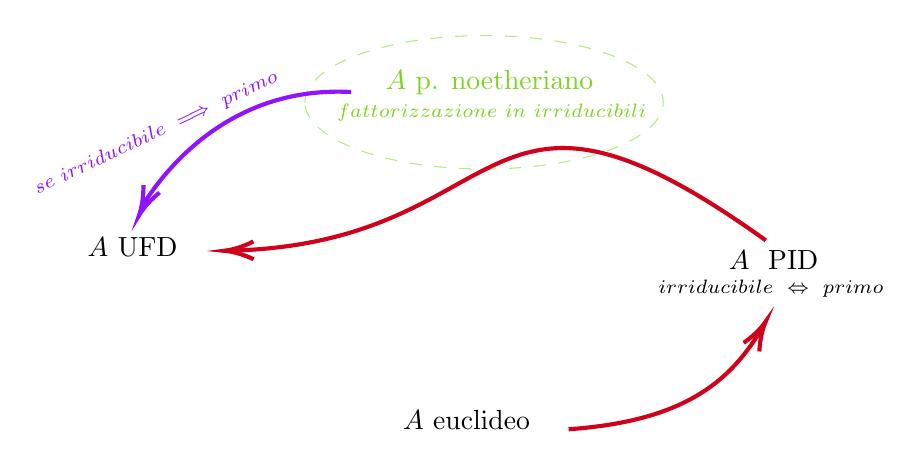
\begin{tikzpicture}[x=0.75pt,y=0.75pt,yscale=-1,xscale=1]
%uncomment if require: \path (0,300); %set diagram left start at 0, and has height of 300

%Shape: Ellipse [id:dp8974017329557005] 
\draw  [color={rgb, 255:red, 184; green, 233; blue, 134 }  ,draw opacity=1 ][dash pattern={on 4.5pt off 4.5pt}] (236,50.95) .. controls (236,33.19) and (274.64,18.8) .. (322.3,18.8) .. controls (369.96,18.8) and (408.6,33.19) .. (408.6,50.95) .. controls (408.6,68.71) and (369.96,83.1) .. (322.3,83.1) .. controls (274.64,83.1) and (236,68.71) .. (236,50.95) -- cycle ;
%Curve Lines [id:da1798398809000128] 
\draw [color={rgb, 255:red, 208; green, 2; blue, 27 }  ,draw opacity=1 ][line width=1.5]    (458,117.5) .. controls (316.71,16.01) and (338.77,119.46) .. (199.12,122.46) ;
\draw [shift={(197,122.5)}, rotate = 359.19] [color={rgb, 255:red, 208; green, 2; blue, 27 }  ,draw opacity=1 ][line width=1.5]    (14.21,-4.28) .. controls (9.04,-1.82) and (4.3,-0.39) .. (0,0) .. controls (4.3,0.39) and (9.04,1.82) .. (14.21,4.28)   ;
%Curve Lines [id:da9422556390169855] 
\draw [color={rgb, 255:red, 144; green, 19; blue, 254 }  ,draw opacity=1 ][line width=1.5]    (258.2,46) .. controls (202.62,43.08) and (170.63,79.7) .. (157.01,101.8) ;
\draw [shift={(156,105.5)}, rotate = 295.17] [color={rgb, 255:red, 144; green, 19; blue, 254 }  ,draw opacity=1 ][line width=1.5]    (14.21,-4.28) .. controls (9.04,-1.82) and (4.3,-0.39) .. (0,0) .. controls (4.3,0.39) and (9.04,1.82) .. (14.21,4.28)   ;
%Curve Lines [id:da6605079993234242] 
\draw [color={rgb, 255:red, 208; green, 2; blue, 27 }  ,draw opacity=1 ][line width=1.5]    (363,208.5) .. controls (417.32,204.62) and (440.59,186.63) .. (456.54,159.08) ;
\draw [shift={(458,156.5)}, rotate = 478.89] [color={rgb, 255:red, 208; green, 2; blue, 27 }  ,draw opacity=1 ][line width=1.5]    (14.21,-4.28) .. controls (9.04,-1.82) and (4.3,-0.39) .. (0,0) .. controls (4.3,0.39) and (9.04,1.82) .. (14.21,4.28)   ;

% Text Node
\draw (273.6,34.4) node [anchor=north west][inner sep=0.75pt]  [color={rgb, 255:red, 126; green, 211; blue, 33 }  ,opacity=1 ] [align=left] {$\displaystyle A$ {p. noetheriano}};
% Text Node
\draw (439,121) node [anchor=north west][inner sep=0.75pt]   [align=left] {$\displaystyle A\ $ {PID}};
% Text Node
\draw (130,115) node [anchor=north west][inner sep=0.75pt]   [align=left] {$\displaystyle A$ {UFD}};
% Text Node
\draw (282,198) node [anchor=north west][inner sep=0.75pt]   [align=left] {$\displaystyle A$ {euclideo}};
% Text Node
\draw (405,135.4) node [anchor=north west][inner sep=0.75pt]  [font=\scriptsize]  {$irriducibile\ \Leftrightarrow \ primo$};
% Text Node
\draw (102.65,88.7) node [anchor=north west][inner sep=0.75pt]  [font=\scriptsize,color={rgb, 255:red, 74; green, 144; blue, 226 }  ,opacity=1 ,rotate=-334.88]  {$\textcolor[rgb]{0.56,0.07,1}{se\ irriducibile\ \Longrightarrow \ primo}$};
% Text Node
\draw (250.2,50.6) node [anchor=north west][inner sep=0.75pt]  [font=\scriptsize,color={rgb, 255:red, 126; green, 211; blue, 33 }  ,opacity=1 ]  {$fattorizzazione\ in\ irriducibili$};
\end{tikzpicture}
\end{equation*}


\section{L'anello degli interi di Gauss}
\subsection{La struttura di anello}
\label{lezione5}
Possiamo sfruttare la teoria appena costruita per studiare una classe molto interessante di anelli. \\
Consideriamo l'insieme
\begin{equation*}
\mathbb{Z}[\sqrt{-k}]\coloneqq \left\{a+b\sqrt{-k} \, \mid \, a,b\in\mathbb{Z}\right\}
\end{equation*}
per $k$ un naturale positivo. Spesso lo indicheremo come $\mathbb{Z}[\omega]$, $\omega = \sqrt{-k}=i\sqrt{k}$. \\ Si tratta di un sottoanello di $\mathbb{C}$, quindi di un dominio di integrità.
\begin{definizione}[Interi di Gauss] 
	Per $\omega=\sqrt{-1}=i$ otteniamo \textbf{l'anello degli interi di Gauss} $\mathbb{Z}[i]$. I suoi elementi hanno forma $z=a+ib$ con $a,b\in\mathbb{Z}$.\footnote{si possono immaginare gli interi di Gauss come il \enquote{reticolo intero} del piano complesso.}
\end{definizione}
\begin{osservazione}[Le unità negli interi di Gauss] 
	Quali sono le unità in $\mathbb{Z}[i]$? Studiamone la struttura, stiamo cercando gli invertibili rispetto al prodotto.
	Dato $z=a+ib\in\mathbb{C}$, si verifica facilmente che il suo inverso moltiplicativo è $w=c+di\in\mathbb{C}$ con
		\begin{equation*}
			c=\frac{a}{a^2+b^2} \ \ \ \ \ d = \frac{-b}{a^2+b^2}
		\end{equation*}
		quindi perché l'inverso di $z\in\mathbb{Z}[i]$ appartenga di nuovo a $\mathbb{Z}[i]$ è necessario che $c$ e $d$ siano interi (ovvero che $a$ e $b$ siano multipli di $a^2+b^2$):
		\begin{equation*}
			a=c(a^2+b^2) \ \ \ \ \ b=(-d)(a^2+b^2)
		\end{equation*}
		Ma svolgendo i calcoli
		\begin{align*}
			a^2+b^2
			&=c^2(a^2+b^2)^2+(-d)^2(a^2+b^2)^2 \\ 
			&=(c^2+d^2)(a^2+b^2)^2
		\end{align*}
		Siccome siamo in un dominio di integrità ($\mathbb{C}$) e tutti gli elementi sono di $\mathbb{Z}$ posso scrivere
		\begin{equation*}
			(b^2+d^2)(a^2+b^2)=1 \implies a^2+b^2=1
		\end{equation*}
		e quindi ho quattro casi per $a$ e $b$, poi determino $c$ e $d$ dalla formula.
		\begin{itemize}
			\item $a=1$, $b=0$, $c=1$, $d=0$
			\item $a=-1$, $b=0$, $c=-1$, $d=0$
			\item $a=0$, $b=1$, $c=0$, $d=1$
			\item $a=0$, $b=-1$, $c=1$, $d=-1$
		\end{itemize}
	Abbiamo quindi visto che:
		\begin{enumerate}
		\item Le unità sono $\pm i$ e $\pm 1$.
		\item Essendo sottoanello di un dominio di integrità (ovvio), $\mathbb{Z}[i]$ è banalmente un dominio di integrità.
	\end{enumerate}
	Posso ottenere in modo più rigoroso e generale lo stesso risultato?
\end{osservazione}
\begin{definizione}
	Sia $z=a+b\omega\in\mathbb{Z}[\omega]$, $\omega=\sqrt{-k}$ per un $k$ intero positivo; definisco la \textbf{norma di $z$} come 
	\begin{equation*}
	N(z)=z\cdot\overline{z}=a^2+kb^2
	\end{equation*}
\end{definizione}
\begin{osservazione}
	Notiamo che la norma così definita non è una funzione aritmetica; è comunque moltiplicativa.
\end{osservazione}
\begin{proposizione}[Caratterizzazione della norma]\
	\begin{enumerate}
		\item $N(z)=0$ se e solo se $z=0$
		\item $N(z\cdot w)=N(z)\cdot N(w)$ per ogni $z,w\in\mathbb{Z}[\omega]$
		\item $z\in\mathbb{Z}[\omega]$ è una unità se e solo se $N(z)=1$
	\end{enumerate}
\end{proposizione}
\begin{proof}\
	\begin{enumerate}
		\item Se $z=0$ ha chiaramente norma nulla, vediamo l'implicazione inversa. Se $a^2+kb^2=0$ per $k$ positivo, $a$ e $b$ devono essere necessariamente nulli.
		\item Si dimostra con calcoli brutali sviluppando $zw$ e $z,w$. Oppure sperando di convincersi abbastanza per non fare i calcoli.
		\item Se $z$ ha norma 1, $z\cdot\overline{z}=1$ e quindi è ovviamente invertibile con inverso il suo coniugato.\\
		Se invece è una delle unità, questo vuol dire che esiste un $x$ con $xz=1$. 
		\begin{equation*}
			N(z)N(x) = N(zx)=N(1)=1
		\end{equation*}
		ed allora $N(z)=1$.
	\end{enumerate}
\end{proof}
\begin{osservazione}
	Sia $z=a+b\omega$ un elemento in $\mathbb{Z}[\omega]$ di norma unitaria, quindi un invertibile, per $\omega=\sqrt{-k}$. Questo vuol dire che:
	\begin{itemize}
		\item[$(k=1)$] caso degli interi di Gauss
		\item[$(k>1)$] $b=0$ ed $a=\pm1$
	\end{itemize}
\end{osservazione}




\subsection{Fattorizzazione unica}
\begin{teorema}
	Ogni $z\in\mathbb{Z}[\omega]$ non nullo si fattorizza in elementi irriducibili.
\end{teorema}
\begin{proof}
	Siano
	\begin{equation*}
		S=\left\{z\neq0, z \in \mathbb{Z}[\omega] \ \text{che non si fattorizzano in irriducibili}\right\}
	\end{equation*}
	\begin{equation*}
		X=\left\{N(z) \, \mid \, z \in S\right\}\subset\mathbb{N}\setminus\left\{0\right\}
	\end{equation*}
	Suppongo $X$ non vuoto, allora ammette un elemento minimo; sia $w$ l'elemento di $S$ per cui $X$ ha tale minimo, in simboli $N(w)=\min X$. \\ Essendo non irriducibile posso scrivere $w=xy$ con né $x$ né $y$ unità.
	\begin{equation*}
	N(w)=N(x)N(y) \ \text{con} \ N(x),N(y)>1 
	\end{equation*}
	Per scelta di $w$ si vede che $x$ ed $y$ non appartengono ad $S$, ma allora si fattorizzano in prodotto di elementi irriducibili, e di conseguenza anche $w$. \\ Allora l'insieme $S$ è vuoto.
\end{proof}
\begin{proposizione}
	Se $k\geq3$ la fattorizzazione in irriducibili esiste (per teorema visto), ma non è unica.
\end{proposizione}
\begin{proof}
	Basta trovare un elemento irriducibile che non sia primo; infatti in un UFD un elemento è irriducibile se e solo se è un primo. \\
	Iniziamo osservando che 2 è irriducibile. Sia $xy=2$, allora $N(x)N(y)=4$: 
	\begin{itemize}
		\item se $N(x)=1$, allora $x$ è una unità
		\item se $N(x)=2$ allora $N(y)=2$, ma 
		\begin{equation*}
		2=N(x)=N(a+b\omega)=a^2+kb^2
		\end{equation*}
		non ha soluzioni intere per $k\geq 3$.
	\end{itemize}
	Dividiamo il resto della dimostrazione in due casi:
	\begin{itemize}
		\item[($k$ pari)] $k=2c=(i\sqrt{k})(-i\sqrt{k})$\\ 2 divide $k=2c$ ma nessuno dei due fattori; si può vedere scrivendo la definizione di divisore. 2 è irriducibile e non primo.
		\item[($k$ dispari)] $k+1=2c=(1+i\sqrt{k})(1-i\sqrt{k})$\\ Analogamente 2 divide $k+1$ ma non i suoi due fattori
	\end{itemize}
\end{proof}
\begin{proposizione}
	Se $k=1,2$ allora $\mathbb{Z}[\omega]$ è euclideo (quindi un UFD).
\end{proposizione}
\begin{proof}
	La norma svolge il ruolo della funzione $f$ nella definizione di dominio euclideo.\\ Siano $z,w\in\mathbb{Z}[\omega]$, voglio mostrare che posso fare la divisione intera.
	Se provassimo a calcolare $z/w$ nel piano complesso otterremmo 
	\begin{equation*}
	\frac{z}{w}=x+y\omega \ \ \ \ x,y\in\mathbb{R}
	\end{equation*}
	ma questo può non appartenere a $\mathbb{Z}[\omega]$. \\ Prendo $q=a+b\omega$ elemento più vicino alla frazione, visto come punto nel piano di Gauss. Allora posso stimare che 
	\begin{equation*}
	|x-a|\leq\frac{1}{2} \ \ \ \ \ \ |y-b|\leq\frac{1}{2}
	\end{equation*}
	\begin{equation*}
	\operatorname{d\left(\frac{z}{w},q\right)}=\sqrt{(x-a)^2+(y-b)^2k}\leq\frac{\sqrt{1+k}}{2}<1
	\end{equation*}
	dove ho usato il fatto che $k<3$. \\ Posso prendere $r=z-wq$, devo però mostrare che ho appena costruito la divisione con resto. Infatti
	\begin{align*}
	N(r)
	&=N(z-wq)=N\left(w(w+y\omega)-qw\right)\\
	&=N\left(w(x+y\omega-q)\right)\\
	&=N\left(w(x+y\omega-a-b\omega)\right)\\
	&=N(x+y\omega-a-b\omega)N(w)<N(w)
	\end{align*}
	dove nell'ultimo passaggio ho sfruttato il calcolo della norma appena svolto.
\end{proof}




\subsection{Alcuni esercizi}
%todo: più esercizi
% Alcuni esercizi: 
% Dire per quali $k \in \mathbb{N}$ l'estensione
% $\mathbb{Z}\left[\sqrt{k}\right]$ è un UFD, per quali è  
% anche un PID, per quali invece è anche un anello euclideo.
% Trovare casi di UFD non PID e casi PID non euclidei. 
% Se non si ha voglia di faticare, basta andare sul manuale di
% Algebra A+B di De Graaf (una lista completa dei PID non UFD
% mi pare sia in uno dei pdf di materiale extra dato da
% Murru).
% danke (s)

\begin{esercizio}[Studio di un anello]
Lavoriamo in $\mathbb{Z}[\sqrt{-5}]$. \\ Vogliamo verificare che 3 e $4+\omega$ ($\omega=\sqrt{-5}$) sono irriducibili, primi tra loro e \textit{non vale l'identità di Bezout}. \\ \\
\begin{itemize}
	\item $N(3)=9$; sia $3=xy$, allora $N(x)N(y)=9$. Ponendo $x=a+b\omega$
	\begin{equation*}
	3=N(x)=a^2+5b^2
	\end{equation*}
	che non ha soluzioni intere. Necessariamente concludiamo che 3 deve essere irriducibile nel nostro anello.
	\item $N(4+\omega)=21$; sia $4+\omega=xy$, allora $N(x)N(y)=21=(3)(7)$. Se lavoriamo come prima otteniamo $N(x)=3$ ed $N(x)=7$, che non danno soluzioni intere.
	\item Hanno divisori comuni? Notiamo che le unità nel nostro dominio sono $\pm1$.
	\begin{equation*}
	3=(1)(3)=(-1)(-3)
	\end{equation*}
	\begin{equation*}
	4+\omega=(1)(4+\omega)=(-1)(-4-\omega)
	\end{equation*}
	Evidentemente i due non si dividono a vicenda, infatti se (ad esempio) 3 dividesse $4+\omega$ potrei scrivere
	\begin{equation*}
	(4+\omega)=3(a+b\omega) \ \ \ \text{per certi $a,b\in\mathbb{Z}$}
	\end{equation*}
	che sicuramente non vale. Se invece $4+\omega$ dividesse 3 potrei scrivere
	\begin{equation*}
	(4+\omega)(a+b\omega)=3 \ \ \ \text{per certi $a,b\in\mathbb{Z}$}
	\end{equation*}
	e svolgendo si trova un sistema senza soluzioni intere.
	\item Vale l'identità di Bezout? Ovvero, esistono $x=x_1+x_2\omega$ ed $y=y_1+y_2\omega$ tali che $x_i,y_i\in\mathbb{Z}$ e $3x+(4+\omega)y=1$?\\ Se esistessero tali $x$ ed $y$ avrei
	\begin{equation*}
		\begin{cases}
			3x_1+4y_1-5y_2=1\\
			3x_2+y_1+4y_2=0
		\end{cases}
	\end{equation*}
	da cui $3(x_1-4x_2-7y_2)=1$, che non ha soluzioni intere.
\end{itemize}
\end{esercizio}
\begin{esercizio}[Non unicità di fattorizzazione]
	Studiamo la fattorizzazione in $\mathbb{Z}[\sqrt{-5}]$ di $z=6$; sappiamo che qui la fattorizzazione non è unica, possiamo ottenere due espressioni differenti di $z$?
	\begin{equation*}
	6 =(3)(2) =(1+\omega)(1-\omega)
	\end{equation*}
	e vedo che sono tutti irriducibili. \\ Si può sfruttare il fatto che $(a-\omega)(a+\omega)=a^2+5$ per ogni $a$ intero, quindi posso ottenere molte fattorizzazioni non uniche sfruttando questo trucco.
	\begin{equation*}
		\begin{array}{lllr}
			\text{per $a=2$} & & &
				9=(2+\omega)(2-\omega)=(3)(3)\\
			\text{per $a=3$} & & &
				14=(3+\omega)(3-\omega)=(2)(7)\\
			\text{per $a=4$} & & &
				21=(4+\omega)(4-\omega)=(3)(7)		
		\end{array}
	\end{equation*}
\end{esercizio}
\begin{esercizio}[Irriducibile non primo]
	Possiamo verificare che 2 è irriducibile e non primo in $\mathbb{Z}[\sqrt{-5}]$. 
	\begin{itemize}
		\item[(irriducibile)] $N(2)=4$, come abbiamo visto più volte se $2=xy$ allora i fattori possono avere norma unitaria (ed allora sono una unità) oppure norma due (ma questo nel nostro anello non è possibile)
		\item[(non primo)] 2 divide $6=(1-\omega)(1+\omega)$ ma non i due fattori
	\end{itemize}
Osserviamo che l'ideale generato da 2 non è primo in $\mathbb{Z}[\sqrt{-5}]$ (in $\mathbb{Z}$ sì), in particolare $\mathbb{Z}[\sqrt{-5}]/(2)$ non è un dominio di integrità.
\end{esercizio}




\chapter{Aritmetica modulare}
L'aritmetica modulare è fondamentale in teoria dei numeri, ad esempio permette di costruire degli importanti criteri: sui residui quadratici, sui numeri primi, e persino nei test di primalità. \\ \\ Vedremo anche le congruenze lineari ed il \textit{teorema cinese del resto}, risultati fondamentali per quanto seguirà. Concluderemo vedendo la struttura degli $\mathbb{Z}_n^*$.



\section{Studio delle classi di resto}
\label{lezione6}
\subsection{La struttura di $\mathbb{Z}_n$}
L'aritmetica modulare lavora negli anelli delle classi di resto
\begin{equation*}
\left(\mathbb{Z}_n,+,0,\cdot,1\right)
\end{equation*}
\begin{osservazione}[Costruzione di un anello di classe di resto]\
	Iniziamo definendo la relazione su $\mathbb{Z}$ 
	\begin{equation*}
	a\sim b \iff n \mid (a-b) 
	\end{equation*}
	per $n$ intero fissato. Ovviamente è una relazione di equivalenza, basta sfruttare le solite proprietà dei divisori. 
	\begin{itemize}
		\item[(riflessiva)] Chiaramente.
		\item[(simmetrica)] Altrettanto ovvio, $n\mid(a-b)$ se e solo se $(a-b)=kn$ per un certo $k$ intero; per invertire la relazione basta prendere $-k$.
		\item[(transitiva)] $n\mid(a-b)$ ed $n\mid(b-c)$ se e solo se $(a-b)=pn$, $(b-c)=qn$ per $p$ e $q$ interi. Dobbiamo ottenere $(a-c)=kn$ per un certo $k$. Dalla prima equazione si vede che $b=a-pn$, sostituendo nella seconda trovo immediatamente
		\begin{equation*}
		(a-pn-c)=qn\implies (a-c)=qn+pn=(q+p)n
		\end{equation*}
	\end{itemize}
	Quindi dire che $a$ e $b$ sono in relazione equivale a dire che hanno lo stesso resto nella divisione euclidea per $n$. \\ Questo caratterizza l'insieme delle classi di equivalenza:
	\begin{equation*}
	\mathbb{Z}_n \simeq \sfrac{\mathbb{Z}}{\sim}
	\end{equation*}
\end{osservazione}
\begin{osservazione}[Costruzione algebrica]
	Possiamo vedere una costruzione più \enquote{algebrica}. Siccome $\mathbb{Z}$ è un PID i suoi ideali sono principali, e sappiamo che hanno forma $(n)=n\mathbb{Z}$. \\ Allora posso costruire la classe di resto tramite le classi laterali
		\begin{equation*}
		\mathbb{Z}_n\simeq\sfrac{\mathbb{Z}}{(n)}\simeq\sfrac{\mathbb{Z}}{n\mathbb{Z}}
		\end{equation*}
		Si vede che $a+(n)=b+(n)$ se e solo se $(a-b)\in(n)$; due elementi appartengono allo stesso ideale se e solo se la loro differenza appartiene al laterale. Quindi le costruzioni sono equivalenti.

\end{osservazione}
\subsection{Struttura additiva}
\begin{proposizione}
	$\left(\mathbb{Z}_n,+\right)$ è un gruppo abeliano ciclico.
\end{proposizione}
\begin{proof}
	Ovvio che sia un gruppo abeliano, altrettanto ovvio che sia ciclico; basta pensare alla struttura in classi di equivalenza.
\end{proof}
\begin{proposizione}
	Ogni gruppo ciclico di ordine $n$ è isomorfo a $\left(\mathbb{Z}_n,+\right)$. 
\end{proposizione}
\begin{proof}
	Se $g$ è ciclico allora è generato da un $g\in G$; per dimostrare la proposizione definisco l'isomorfismo
	\begin{align*}
	\phi:(\mathbb{Z}_n,+)&\longrightarrow (G,\cdot)\\
	k &\longmapsto g^k
	\end{align*}
	\begin{itemize}
		\item[(ben definita)] Siano $[a]=[b]\in\mathbb{Z}_n$ la stessa classe (con due rappresentanti diversi), per due certi $a,b\in\mathbb{Z}$; devo mostrare che la funzione non dipende dal rappresentante della classe. Notiamo che se $a$ e $b$ sono nella stessa classe allora $n$ divide la loro differenza. Questo scritto tramite la divisione euclidea (ad esempio) diventa $a-b=kn$, cioè $a=kn+b$, per un certo $k\in\mathbb{Z}$.
		\begin{align*}
		\phi([a])&=g^{[a]}=g^{[kn+b]}=g^{[kn]}g^{[b]}=1\cdot g^{[b]}\\
		&=g^{[b]}=\phi([b])
		\end{align*}
		Si noti l'utilizzo della struttura ciclica di $G$.
		\item[(omomorfismo)] Banalmente vero.
		\item[(iniettiva)] Vediamo che $\ker \phi = \left\{0\right\}$: se $x \in \ker \phi$ allora $\phi(x) = g^x = 1$, quindi $n \mid x$. Dev'essere che $x \equiv 0 \Mod n$, ovvero $x \equiv 0 \in \mathbb{Z}_n$. 
		\item[(suriettiva)] Per un fatto noto di algebra una funzione iniettiva tra insiemi finiti della stessa dimensione è anche suriettiva, ed i nostri insiemi sono ciclici.
	\end{itemize}
	Avendo trovato un isomorfismo abbiamo ottenuto la tesi.
\end{proof}
\begin{definizione}
	L'insieme di interi $\left\{a_1,\dots,a_n\right\}$ è un \textbf{sistema completo di residui modulo $n$} (oppure ancora \textbf{di rappresentanti di $\mathbb{Z}_n$}) se
	\begin{enumerate}
		\item per $i\neq j$, $a_i\nequiv a_j \Mod(n)$
		\item per ogni $a$ in $\mathbb{Z}_n$ esiste un indice $i$ tale che $a\equiv a_i \Mod(n)$
	\end{enumerate}
Il \textbf{sistema canonico di rappresentanti} di $\mathbb{Z}_n$ è
\begin{equation*}
1,2,\dots,n-1
\end{equation*}
\end{definizione}
\begin{proposizione}
	Siano $m,n$ in $\mathbb{Z}$ tali che $m$ divide $n$, allora la funzione
	\begin{align*}
	\phi:\mathbb{Z}_n&\longrightarrow\mathbb{Z}_m\\
	[a]_n&\longmapsto[a]_m
	\end{align*}
	è un omomorfismo suriettivo.
\end{proposizione}
\begin{proof}\
	\begin{itemize}
		\item[(ben definita)] Chiaramente se $[a]_n=[b]_n$ allora $n$ divide $a-b$, e quindi anche $m$ li divide; sono nella stessa classe anche rispetto ad $m$.
		\item[(omomorfismo)] Ovvio per struttura delle classi.
		\item[(suriettiva)] Ogni $[x]_m$ ha una controimmagine, $[x]_n$. Poiché $m$ divide $n$ allora è necessariamente più piccolo, quindi non posso \enquote{perdere classi}, o in altre parole non ho una riduzione dei rappresentanti. 
	\end{itemize}
\end{proof}
\begin{proposizione}
	\label{prod_ciclici}
	Sia $n=ab$ con $a,b\in\mathbb{Z}$ coprimi, allora 
	\begin{equation*}
	(\mathbb{Z}_n,+)\simeq(\mathbb{Z}_a,+)\times(\mathbb{Z}_b,+)
	\end{equation*}
\end{proposizione}
\begin{proof}
	Definiamo le funzioni
	\begin{equation*}
		\begin{array}{rll}
			\phi \; \colon & \mathbb{Z}_n & \longrightarrow\mathbb{Z}_a \times \mathbb{Z}_b\\
			& [x]_n & \longmapsto\left([x]_a,[x]_b\right) \\
			 & & \\
			\phi_a \; \colon & \mathbb{Z}_n & \longrightarrow \mathbb{Z}_a \\
			& [x]_n & \longmapsto[x]_a\\
			 & & \\
			\phi_b \; \colon & \mathbb{Z}_n & \longrightarrow\mathbb{Z}_b \\
			& [x]_n & \longmapsto[x]_b
		\end{array}
	\end{equation*}
	Osserviamo subito che $\phi([x]_n)=\left(\phi_a([x]_n),\phi_b([x]_n)\right)$:
	\begin{equation*}
	%https://tikzcd.yichuanshen.de/#N4Igdg9gJgpgziAXAbVABwnAlgFyxMJZABgBoBGAXVJADcBDAGwFcYkQAdDgW3pwAsARoOAAtAL4B9QuNLpMufIRTlSxanSat2XXgOFip9ELPnY8BIqoBMGhizaJOPPkJETJgk3JAZzSomsKOy1HZz03Q0l6LjxueF1XAw8vcQ0YKABzeCJQADMAJwhuJDIQHAgkVRBGekEYRgAFBQtlECwwbFgQGnttJy40fixo73yiksQyiqQgmrqG5v9LJw6utl7QnQ4hkdSfQuLSmhnEAGYaWvqmloDVzqxuzYdt3bGQQ8nq04vy+ixGOx+BAIABrd6fWYnSrnE7-QFOYFgkyUcRAA
	\begin{tikzcd}
	& \mathbb{Z}_a \arrow[rd, hook] &                                \\
	\mathbb{Z}_n \arrow[ru, "\phi_a" description] \arrow[rd, "\phi_b" description] \arrow[rr, "\phi" description] &                               & \mathbb{Z}_a\times\mathbb{Z}_b \\
	& \mathbb{Z}_b \arrow[ru, hook] &                               
	\end{tikzcd}
	\end{equation*}
	Siccome $a$ e $b$ dividono $x$, per quanto appena dimostrato $\phi_a$ e $\phi_b$ sono morfismi suriettivi, ed in quanto composizione di morfismi - tra cui l'inclusione - anche $\phi$ è un morfismo.
	\begin{itemize}
		\item[(iniettiva)] Studiamo il suo nucleo.
		\begin{align*}
		\ker(\phi)&=\left\{[x]_n\in\mathbb{Z}_n \, \mid \, \phi([x]_n)=\left([0]_a,[0]_b\right)\right\}\\
		&=\left\{[x]_n\in\mathbb{Z}_n \, \mid \, \phi([x]_n)=\big(\phi_a([0]_n),\phi_b([0]_n)\big)\right\}\\
		&=\left\{[x]_n\in\mathbb{Z}_n \, \mid \, \phi_a([x]_n)=0,\phi_b([x]_n)=0\right\}\\
		&=\left\{[0]_n\in\mathbb{Z}_n\right\}
		\end{align*}
		L'ultimo passaggio in particolare vale perché $a$ e $b$ sono coprimi, quindi il loro minimo comune multiplo è $ab=n$. Poiché entrambi valgono zero insieme ottengo necessariamente la tesi.
		\item[(suriettiva)] La cardinalità del gruppo ciclico $\mathbb{Z}_n$ è $n=ab$, che è il prodotto delle cardinalità di $\mathbb{Z}_a$ e $\mathbb{Z}_b$, concludiamo allo stesso modo di prima. Si noti che $\mathbb{Z}_a\times \mathbb{Z}_b$ è ciclico se $a$ e $b$ sono coprimi.
	\end{itemize}
\end{proof}
\begin{teorema}[Decomposizione in gruppi ciclici additivi] Sia $n$ un qualunque elemento $n>1$ in $\mathbb{Z}$, posso decomporlo in primi $n=p_1^{e_1}\dots p_t^{e_t}$.
	Allora vale 
	\begin{equation*}
	(\mathbb{Z}_n,+)\simeq(\mathbb{Z}_{p_1^{e_1}},+)\times\dots\times(\mathbb{Z}_{p_t^{e_t}},+)
	\end{equation*}
\end{teorema}
\begin{proof}
	Posso usare la Proposizione \ref{prod_ciclici} lavorando per induzione su $t$. Chiaramente le ipotesi della proposizione sono soddisfatte, perché ${p_i^{e_i}}$ è coprimo con ${p_j^{e_j}}$ per $i\neq j$.
\end{proof}




\subsection{Struttura moltiplicativa}
\begin{proposizione}
	In $\left(\mathbb{Z}_n,+,\cdot\right)$ un elemento non nullo è invertibile rispetto al prodotto. Questo equivale a dire che per ogni $a$ in $\mathbb{Z}_n$ vale una delle seguenti:
	\begin{enumerate}
		\item $a$ ed $n$ sono coprimi
		\item $a$ è un divisore dello zero
	\end{enumerate}
\end{proposizione}
\begin{proof}
	$a$ ed $n$ sono coprimi equivale a dire che (per Bezout) esistono $x,y\in\mathbb{Z}$ con $ax+yn=1$, che equivale a dire
	\begin{equation*}
	ax\equiv1\Mod(n)
	\end{equation*}
	Invece $\MCD(a,n)=d>1$ equivale a dire $a=dk_a$, $n=dk_n$ per $k_a,k_b\in\mathbb{Z}$ e $k_n\neq0$. Dunque 
	\begin{equation*}
	ak_n=(dk_a)k_n=k_an\equiv0\Mod(n)
	\end{equation*}
\end{proof}
\begin{osservazione}[Gruppo delle unità]
	Notiamo che $\left(\mathbb{Z}_n^*,\cdot\right)$ è un gruppo moltiplicativo di $\mathbb{Z}_n$, detto anche \textbf{gruppo delle unità modulo $n$}. \\ Diciamo $\varphi$ la funzione di Eulero, che abbiamo già incontrato.
	\begin{align*}
	\varphi: \mathbb{N}&\longrightarrow \mathbb{N}\\
	n &\longmapsto |\mathbb{Z}_n^*|
	\end{align*}
	Allora possiamo dire per $a$ e $b$ coprimi ed $n=ab$
	\begin{align*}
	\phi:\mathbb{Z}^*_n&\longrightarrow\mathbb{Z}^*_a\times \mathbb{Z}^*_b\\
	[x]_n&\longmapsto\left([x]_a,[x]_b\right)
	\end{align*}
	è un isomorfismo.
	\begin{itemize}
		\item[(ben definita)] Ovvio, basta riadattare la dimostrazione già vista.
		\item[(omomorfismo)] 
		\begin{align*}
		\phi\left([x]_n[y]_n\right)&=\phi\left([xy]_n\right)=\left([xy]_a,[xy]_b\right)\\
		&=\left([x]_a[y]_a,[x]_b[y]_b\right)=\phi\left([x]_n\right)\phi\left([y]_n\right)
		\end{align*}
		L'ultima uguaglianza andrebbe formalizzata meglio ripercorrendo i calcoli al contrario. \\
		\item[(iniettiva)] Il nucleo di $\phi$ sono gli elementi mandati nell'elemento neutro in arrivo, quindi $1$.\footnote{stiamo usando una notazione moltiplicativa per i gruppi; in poche parole, solitamente scriviamo l'operazione come $+$ e di conseguenza il neutro come $0$ ma è possibile usare la moltiplicazione (ed in quel caso l'elemento neutro sarà ovviamente $1$).}
		Vediamo un fatto generale per la nostra situazione, $[x]_n$ è invertibile se e solo se lo sono $\left([x]_a\right)$ ed $\left([x]_b\right)$. Infatti assumo sia invertibile e pongo $[z]_n=[x]^{-1}_n$, allora
		\begin{align*}
		\left([z]_a[x]_a,[z]_b[x]_b\right)&=\left([z]_a,[z]_b\right)\left([x]_a,[x]_b\right)\\
		&=\phi([z]_n)\phi([x]_n)\\
		&=\phi([1]_n)=\left([1]_a,[1]_b\right)
		\end{align*}
		Se invece sono invertibili $\left([x]_a\right)$ ed $\left([x]_b\right)$ esistono $[z]_a$ e $[z]_b$ loro inversi, quindi basta sfruttare il fatto che le funzioni $\phi_a$ e $\phi_b$ siano omomorfismi. \\ Otteniamo subito che la funzione è iniettiva.
		\item[(suriettiva)] Come le altre volte.
	\end{itemize}
\end{osservazione}
\begin{proposizione}\
	\begin{enumerate}
		\item La funzione di Eulero è una funzione aritmetica moltiplicativa.
		\item Per $p$ primo $\varphi(p)=p-1$.
		\item $\varphi(p^e)=p^{e-1}(p-1)$ per $p$ primo.
	\end{enumerate}
	Allora nota la fattorizzazione di un $n$ intero posso calcolare il valore di $\phi(n)$; il problema sarà proprio fattorizzare $n$.
\end{proposizione}
\begin{proof}\
	\begin{enumerate}
		\item Segue da quanto appena visto, per $n=ab$ con $a,b$ coprimi
		\begin{align*}
		\varphi(ab)&=\varphi(n)=|\mathbb{Z}_n^*|=|\mathbb{Z}_a^*\times\mathbb{Z}_b^*|\\
		&=|\mathbb{Z}_a^*|\cdot|\mathbb{Z}_b^*|=\varphi(a)\varphi(b)
		\end{align*}
		\item Ovvio per definizione di funzione di Eulero.
		\item Dato $a\in\mathbb{N}$ ed $a\in[1,p^e]$ si ha che
		\begin{align*}
		\MCD(a,p^e)=1&\iff \text{$p$ non divide $a$}\\
		\MCD(a,p^e)\neq1&\iff \text{$p$ divide $a$}
		\end{align*}
		quindi $\varphi(p^e)$ è
		\begin{align*}
		p^e-\left|\left\{r\in\mathbb{N} \, \mid \, 1\leq r\leq p^e \ \text{e $p$ divide $r$}\right\}\right|
		\end{align*}
		Notando che l'insieme a destra è quello dei multipli di $p$ (quindi $p,2p,3p,\dots,p^{e-1}p$), otteniamo che 
		\begin{equation*}
		\varphi(p^e)=p^e-p^{e-1}=p^{e-1}(p-1)
		\end{equation*}
	\end{enumerate}
\end{proof}
\begin{esempio}
	\begin{align*}
	\varphi(9)
	&=\varphi(3^2)\\
	&=3^{2-1}(3-1)=(3)(2)=6
	\end{align*}
\end{esempio}
\begin{teorema}[Piccolo teorema di Fermat]
	\label{piccolo_fermat}
	Per ogni $a\in\mathbb{Z}_p^*$ con $p$ primo, vale la seguente formula.
	\begin{equation*}
	a^{p-1}\equiv1\Mod(p)
	\end{equation*}
\end{teorema}
\begin{proof}[Dimostrazione \enquote{elementare}]
	Dimostriamolo per induzione su $a$.
	\begin{enumerate}
		\item[($a=1$)]La tesi è $1^{p-1}=1\equiv1\Mod(p)$, che è banalmente vera. 
		\item[($a+1$)] Riscriviamo facilmente l'ipotesi induttiva.
		\begin{equation*}
		a^{p-1}\equiv1\Mod(p)\iff a^p\equiv a\Mod(p)
		\end{equation*}
		Dimostriamo il passo $a+1$-esimo. Il fatto che $(a+1)^p\equiv(a^p+1)\Mod(p)$ è ben noto dall'algebra, basta scrivere la formula di Newton per l'espansione della potenza $p$. Questo implica subito la tesi sfruttando l'ipotesi induttiva:
		\begin{align*}
		(a)^{p}\equiv(a)\Mod(p) \ \ \ \ \ \ &\text{ipotesi induttiva}\\
		(a+1)^p\equiv(a^p+1)\Mod(p) \ \ \ \ \ \ &\text{fatto noto}\\
		\Longrightarrow (a+1)^{p}\equiv (a^p+1) \equiv (a+1)\mod(p)
		\end{align*}
	\end{enumerate}
\end{proof}
\begin{proof}[Dimostrazione \enquote{avanzata}] 
	Si può dimostrare anche come banale conseguenza delle proprietà della funzione di Eulero e della teoria che abbiamo appena visto. \\ Non lo faremo, ma è possibile. 
\end{proof}
\begin{teorema}[Teorema di Eulero]
	\label{eulero}
	Per ogni $a\in\mathbb{Z}_n^*$ vale la seguente formula.
	\begin{equation*}
	a^{\varphi(n)}\equiv 1 \Mod(n)
	\end{equation*}
\end{teorema}
\begin{proof}
	Ricordiamo che $|\mathbb{Z}^*_n| = \varphi(n)$, da cui poiché $\langle a\rangle \leq \mathbb{Z}^*_n$ dev'essere che l'ordine di $\langle a\rangle$ è $o(a)$ divisore di $ |\mathbb{Z}^*_n|$, questo per teorema di Lagrange. Si conclude per definizione di ordine che $1^k = a^{o(a)k} = a^{\varphi(n)}$, dove $k \cdot o(a)=|\mathbb{Z}^*_n|$. 
\end{proof}




\subsection{Congruenze lineari e teorema cinese del resto}
Diciamo \textbf{congruenze lineari} equazioni del tipo
\begin{equation*}
ax\equiv b\Mod(n)
\end{equation*}
Notiamo alcune cose:
\begin{enumerate}
	\item Se $a$ è invertibile (in $\mathbb{Z}_n$), ovvero se $a$ ed $n$ sono coprimi (per caratterizzazione vista), notiamo subito che si risolve ponendo
	\begin{equation*}
	x\equiv a^{-1}b\Mod(n)
	\end{equation*}
	\item Se $a$ non è invertibile, ovvero $a$ ed $n$ hanno massimo comune divisore $d\neq1$, si risolve se e solo se $d$ divide $b$. In questo caso infatti si pone $a'=\frac{a}{d}$, $b'=\frac{b}{d}$, $n'=\frac{n}{d}$ (nota: $a'$ ed $n'$ sono coprimi).\\
	Questo perché il problema equivale a risolvere l'equazione diofantina 
	\begin{equation*}
	ax+ny=b
	\end{equation*}
	nelle incognite $x$ ed $y$, e se $d$ divide $b$ abbiamo che $d$ divide $ax+ny$.
	\begin{equation*}
	a'x+n'y=b' \iff a'x\equiv b'\Mod(n)
	\end{equation*}
\end{enumerate}
Poniamo invece di voler risolvere \textit{un sistema} di $k$ congruenze lineari.
\begin{equation*}
\begin{cases}
a_1x&\equiv b_1\Mod(n_1)\\
&\,\vdots\\
a_kx&\equiv b_k\Mod(n_k)
\end{cases}
\end{equation*}
Allora ogni equazione deve innanzi tutto essere risolvibile secondo il criterio appena studiato, 
\begin{equation*}
\MCD(a_i,n_i)\mid b_i \ \ \forall i \in \left\{1, \dots, k\right\}
\end{equation*}
ma stavolta non è sufficiente a garantire l'esistenza di una soluzione.
\begin{controesempio}
	Le condizioni non sono sufficienti a garantire l'esistenza di una soluzione. Si consideri il seguente sistema lineare 
	\begin{equation*}
	\begin{cases}
		x\equiv 2\Mod(4)\\
		x\equiv 1\Mod(2)
	\end{cases}
	\end{equation*}
	La prima ci dice che $x = 4k + 2$ e quindi ha come soluzioni numeri pari; la seconda invece dice che $x = 2k + 1$, ovvero ha soluzioni dispari. Un numero intero non può essere sia pari che dispari: la soluzione non esiste. \\ \\ Questo è evidentemente un caso non raro; ogni equazione di per sé ha (sempre) un insieme di soluzioni e nulla mi vieta di mettere a sistema due equazioni che non abbiano alcuna soluzione in comune.
\end{controesempio}
\begin{esempio}
	Proviamo a lavorare sulla congruenza lineare
	\begin{equation*}
	3x\equiv5\Mod6
	\end{equation*}
	dove $a$ ed $n$ non sono coprimi. Siccome il loro massimo comune divisore 3 non divide $b$ ci troviamo in un caso dove non esiste soluzione. Potremmo confermare ulteriormente la cosa prendendo tutti gli interi nella classe di resto $\mathbb{Z}_6$ e provando a moltiplicarli per 3, nessuno dei possibili prodotti darà mai come risultato la classe di 5.
\end{esempio}
\begin{osservazione}
	Consideriamo ad esempio il sistema di due equazioni
	\begin{equation*}
	\begin{cases}
	a_1x\equiv b_1\Mod(n_1)\\
	a_2x\equiv b_2\Mod(n_2)
	\end{cases}
	\end{equation*}
	che sotto le condizioni viste può essere riscritto come 
	\begin{equation*}
	\begin{cases}
	x\equiv c_1\Mod(n_1)\\
	x\equiv c_2\Mod(n_2)
	\end{cases}
	\end{equation*}
	\begin{equation*}
	\begin{cases}
	x=c_1+kn_1'\\
	x=c_2+hn_2'
	\end{cases}
	\end{equation*}
	Otteniamo l'equazione nelle incognite $h,k$
	\begin{equation*}
	c_1-c_2=hn_2'-kn_1'
	\end{equation*}
	che per Bezout ha soluzione se e solo se $\MCD(n_1',n_2') \mid c_1-c_2$.
\end{osservazione}
\begin{teorema}[Teorema cinese del resto]
	Siano $m,n\in\mathbb{Z}$ coprimi ed $a,b\in\mathbb{Z}$. Allora il sistema 
	\begin{equation*}
	\begin{cases}
	x\equiv a\Mod(m)\\
	x\equiv b\Mod(n)
	\end{cases}
	\end{equation*}
	ha una ed una sola soluzione in modulo $mn$.
\end{teorema}
\begin{proof}
	Consideriamo la funzione 
	\begin{align*}
	\varphi:\mathbb{Z}&\longrightarrow\mathbb{Z}_m\times\mathbb{Z}_n\\
	x&\longmapsto\left([x]_m,[x]_n\right)
	\end{align*}
	Se è suriettiva ottengo subito che esiste un $x\in\mathbb{Z}$ tale che $\varphi(x)=\left([a]_m,[b]_n\right)$, e questa è la soluzione del sistema.
	\begin{itemize}
		\item[(ben definita)] Già visto.
		\item[(omomorfismo)] Ovvio.
		\item[(iniettiva?)] Non è iniettiva, il nucleo è non banale.
		\begin{align*}
		\ker(\varphi)&=\left\{x\in\mathbb{Z} \, \middle| \, x\equiv 0 \Mod(n),x \equiv 0 \Mod(m)\right\}\\
		&=\left\{x\in\mathbb{Z} \, \middle| \, \text{$mn$ divide $x$}\right\}\\
		&=(mn)\mathbb{Z}
		\end{align*}
		Si noti che in questo punto stiamo usando l'ipotesi $m$ ed $n$ coprimi.
		\item[(suriettiva)]
		La funzione è palesemente suriettiva per costruzione, tutto lo spazio di arrivo viene coperto.
	\end{itemize}
	Il nucleo è non banale, ma la mappa è ben definita e suriettiva; posso sfruttare il primo teorema di isomorfismo tra anelli ed ottengo l'isomorfismo
	\begin{equation*}
	\sfrac{\mathbb{Z}}{\ker(\varphi)}\simeq\mathbb{Z}_m\times\mathbb{Z}_n\simeq\mathbb{Z}_{mn}
	\end{equation*}
	Allora se $x$ è soluzione, tutte le soluzioni hanno forma 
	\begin{equation*}
	x+k(mn) \ \ \ \ k\in\mathbb{Z}
	\end{equation*}
	ovvero ho esistenza ed unicità di soluzione in $\mathbb{Z}_{mn}$. Questo perché le ipotesi del teorema mi mettono nella situazione di esistenza della soluzione che abbiamo appena studiato.
\end{proof}
\begin{proposizione}
	Sia data la fattorizzazione di $n$
	\begin{equation*}
	n=\prod_{i=1}^{n}{p_i}^{{e_i}}=\alpha\cdot\beta\cdot\ \dots \ \omega
	\end{equation*}
	dove $\alpha,\beta,\dots,\omega$ sono i fattori (i primi, esponente incluso). Allora 
	\begin{equation*}
	\mathbb{Z}_n\simeq\mathbb{Z}_{\alpha}\times\ \dots \ \times\mathbb{Z}_{\omega}
	\end{equation*}
	%inserire gli alpha è stato necessario per grane varie di latex con i pedici
	In particolare abbiamo anche che 
	\begin{equation*}
	\mathbb{Z}_n^*\simeq\mathbb{Z}_{\alpha}^*\times\ \dots \ \times\mathbb{Z}_{\omega}^*
	\end{equation*}
\end{proposizione}
\begin{proof}
	Si svolge considerando il morfismo
	\begin{align*}
	\varphi:\mathbb{Z}&\longrightarrow\mathbb{Z}_{\alpha}\times\ \dots \ \times\mathbb{Z}_{\omega}\\
	x&\longmapsto\left([x]_{\alpha},\dots,[x]_{\omega}\right)
	\end{align*}
	e dimostrando che è isomorfismo.
\end{proof}
\begin{teorema}[Teorema cinese del resto, generale]
	Siano $n_1,\dots,n_k\in\mathbb{Z}$ due a due coprimi ed $a_1,\dots,a_k\in\mathbb{Z}$. Allora il sistema 
	\begin{equation*}
	\begin{cases}
	x&\equiv a_1\Mod(n_1)\\
	&\,\vdots\\
	x&\equiv a_k\Mod(n_k)
	\end{cases}
	\end{equation*}
	ha una ed una sola soluzione in modulo $n_1\dots n_k$.
\end{teorema}




\section{Classi di resto come gruppi ciclici}
\subsection{La struttura ciclica di $\mathbb{Z}^*_p$}
\label{lezione7}
Ovviamente prenderemo come $p$ un primo di $\mathbb{Z}$.
\begin{proposizione}
	Sia $G=\left\{g_1,\dots,g_s\right\}$ un gruppo abeliano finito, sia $n$ il massimo degli ordini dei suoi elementi. \\ Allora l'ordine di ogni elemento divide $n$.\footnote{non è scontato che $n$ sia uguale ad $s$, anzi se il gruppo non è ciclico vale $n<s$.}
\end{proposizione}
\begin{proof}
	Sia $g\in G$ l'elemento di ordine $n$ massimo e sia $h\in G$ di ordine $m$ generico. Supponiamo per assurdo che $m$ non divida $n$.\\ \\
	Se $m$ ed $n$ fossero coprimi allora $gh\in G$ avrebbe ordine $mn$, ma questo è in contraddizione con la scelta di $n$. Allora non sono coprimi. Definiamo $\nu_p(x)$ come la valutazione $p$-adica di $x$, ovvero la massima potenza di $p$ che divide $x$; l'idea è avere un primo che divida entrambi con potenze diverse. Sia allora $p$ primo con $\nu_p(m)=e$, $\nu_p(n)=f$, evidentemente $0<f<e$. Consideriamo l'elemento $g^{p^f}$, verifichiamo facilmente che ha ordine $\frac{n}{p^f}$. 
	\begin{equation*}
	\left(g^{p^f}\right)^{\sfrac{n}{p^f}}=g^n=1
	\end{equation*}
	Analogamente $h^{\sfrac{m}{p^e}}$ ha ordine $p^e$.
	\begin{equation*}
	\left(h^{\sfrac{m}{p^e}}\right)^{p^e}=h^m=1
	\end{equation*}
	Siccome questi due ordini sono coprimi, $\left(g^{p^f}\right)(h^{\sfrac{m}{p^e}})$ appartiene a $G$ - perché è un gruppo - ed ha ordine $\frac{n}{p^f}p^e=p^{e-f}n>n$; questo contraddice di nuovo la scelta di $n$.
\end{proof}
\begin{teorema}
	Sia $f\in\mathbb{Z}_p[x]$ polinomio non costante e di grado $d$ (nella variabile $x$), allora ha al più $d$ radici in $\mathbb{Z}_p$.
\end{teorema}
\begin{proof}
	Iniziamo ricordando che per teorema di Ruffini $f(a)=0$ se e solo se $(x-a)$ divide $f$. Procediamo per induzione su $d$.
	\begin{itemize}
		\item[($d=1$)] Banale, sono nel caso $f(x)=ax+b$ per $a$ non-zero ed $a,b\in\mathbb{Z}_p$. \\ Ovviamente ho una sola radice: $-ba^{-1}$.
		\item[($d+1$)] Sia ora 
		\begin{equation*}
		f(x)=c_0+\ \dots\ +c_{d+1}x^{d+1}  \ \ \ \ \ \ \ \ c_i\in\mathbb{Z}_p,\ c_{d+1}\neq 0
		\end{equation*}
		Se non ha radici ottengo la tesi, altrimenti esiste un $a\in\mathbb{Z}_p$ tale che $f(a)=0$. In questo caso posso riscrivere $f$ come 
		\begin{equation*}
		f(x)=(x-a)g(x)
		\end{equation*}
		per un certo polinomio $g(x)\in\mathbb{Z}_p[x]$ di grado $d$, su cui posso usare l'ipotesi induttiva.
	\end{itemize}
\end{proof}
\begin{teorema}
	$\left(\mathbb{Z}_p^*,\cdot\right)$ è un gruppo ciclico.
\end{teorema}
\begin{proof}
	Sia $n$ il massimo degli ordini degli $i$ compresi tra $1$ e $p-1$, voglio mostrare che $n=p-1$; in questo modo otterrei che esiste almeno un elemento di ordine $p-1$ e da qui la tesi. \\ Sicuramente $n\leq p-1$ ed $n$ divide $p-1$, in particolare ogni elemento $a$ del gruppo ha ordine $m$ che divide $n$ e quindi
	\begin{equation*}
	a^m\equiv a^n\equiv 1\Mod(p) 
	\end{equation*}
	Questo vuol dire che $x^n-1\in\mathbb{Z}_p[x]$ ha almeno $p-1$ soluzioni, quindi $p-1\leq n$.
\end{proof}
\begin{osservazione}
	Anche se sappiamo che $\left(\mathbb{Z}_p^*,\cdot\right)$ è ciclico non sempre è facile trovare un suo generatore. 
	\begin{equation*}
	\left(\mathbb{Z}_p^*,\cdot\right)\simeq\left(\mathbb{Z}_{p-1},+\right)
	\end{equation*}
\end{osservazione}

\subsection{La struttura ciclica di $\mathbb{Z}_n^*$}
Abbiamo visto che 
\begin{itemize}
	\item considerando l'operazione di somma $\left(\mathbb{Z}_n,+\right)$ è ciclico per ogni $n$; più in particolare ogni gruppo ciclico finito è isomorfo ad un $\left(\mathbb{Z}_n,+\right)$
	\item considerando l'operazione di prodotto $\left(\mathbb{Z}_p^*,\cdot\right)$ è ciclico per $p$ primo, ma non per tutti gli $n$ $\left(\mathbb{Z}_n^*,\cdot\right)$ è ciclico
\end{itemize}
Come possiamo caratterizzare gli $n$ per cui otteniamo un $\left(\mathbb{Z}_n^*,\cdot\right)$ ciclico?
\begin{definizione}
	Un $a\in\mathbb{Z}_n^*$ si dice \textbf{radice primitiva modulo $n$} se ha ordine $\varphi(n)$
	, ovvero se è un generatore di $\mathbb{Z}_n^*$.
\end{definizione}
\begin{esempio}
	Osserviamo alcuni esempi di radici primitive.
	\begin{itemize}
		\item $\mathbb{Z}_2^*=\left\{1\right\}$, è ciclico
		\item $\mathbb{Z}_4^*=\left\{1,3\right\}$, è ciclico; oltretutto $\left(\mathbb{Z}_4^*,\cdot\right)\simeq\left(\mathbb{Z}_{2},+\right)$
	\end{itemize}
\end{esempio}
\begin{proposizione}
	Per $n=2^k$ pari con $k>2$ e per $a\in\mathbb{Z}_n^*$ si ha 
	\begin{equation*}
	a^{2^{k-2}}\equiv1\Mod\left(2^k\right)
	\end{equation*} 
\end{proposizione}
\begin{proof}
	Procediamo per induzione su $k$, l'ipotesi induttiva è 
	\begin{equation*}
	a^{2^{k-2}}\equiv1\Mod2^k \iff a^{2^{k-2}}=1+t2^k \ \ \ \ \ t \in \mathbb{Z}
	\end{equation*}
	Per provarlo bastano pochi calcoli.
	\begin{align*}
	a^{2^{(k+1)-2}}&=a^{2^{k-2}\cdot2}=\left(a^{2^{k-2}}\right)^2=\left(1+t2^k\right)^2\\
	&= 1+t2^{k+1}+t^22^{2k}\equiv1\Mod2^{k+1}
	\end{align*}
\end{proof}
\begin{controesempio}
	Se non ponessi $k>2$ avrei palesemente una situazione falsa. Prendiamo ad esempio $k=2$ e lavoriamo in
	\begin{equation*}
	\mathbb{Z}_4^*=\left\{1,3\right\}
	\end{equation*}
	siamo quindi sotto le ipotesi (\enquote{corrette}) del teorema. Abbiamo chiaramente una tesi falsa, perché
	\begin{equation*}
	3^{2^{2-2}}=3^{1}=3\nequiv1\Mod\left(2^2\right)
	\end{equation*} 
\end{controesempio}
\begin{esempio}
	Lavorando in $\mathbb{Z}_8^*=\left\{1,3,5,7\right\}$, per $k=3$, ottengo 
	\begin{equation*}
	1^2\equiv3^2\equiv5^2\equiv7^2\equiv1\Mod8
	\end{equation*}
	Posso ripetere lo stesso ragionamento per $n=2^k$ e $k>2$ generico.
\end{esempio}
\begin{corollario}
	$\left(\mathbb{Z}_{2^k}^*,\cdot\right)$ è ciclico se e solo se $k=1,2$.
\end{corollario}
\begin{proof}
	Se $k=1,2$ il gruppo è palesemente ciclico. \\ Sia allora $\left(\mathbb{Z}_{2^k}^*,\cdot\right)$ gruppo ciclico, voglio mostrare che per $k\geq3$ la tesi è falsa. Ma questo è ovvio, siamo sotto le condizioni della proposizione precedente con $n=2^k$; allora sappiamo che per $k>2$
	\begin{equation*}
	a^{2^{k-2}}\equiv1\Mod2^k
	\end{equation*}
	e palesemente il gruppo non può essere ciclico. Ad esempio per la non esistenza di un elemento di ordine $\varphi(2^k)$, cioè di ordine $2^{k-1}$. Infatti supponiamo che esista un elemento $g$ di tale ordine, questo avrebbe 
	\begin{align*}
	g^{2^{k-1}}
	&=g^{2^{k-2}2}=\left(g^{2^{k-2}}\right)^2\\
	&=\left(1\right)^2=1
	\end{align*}
	Ma nel calcolo abbiamo svolto un passaggio interessante; sfruttando la suddetta relazione si dimostra che elevato alla $2^{k-2}$ restituisce 1, e per richiesta di minimalità nella definizione di ordine questo è un assurdo.
\end{proof}
\begin{proposizione}
	Sia $g$ generatore di $\mathbb{Z}_p^*$, allora $g$ o $g+p$ è un generatore di $\mathbb{Z}_{p^2}^*$.
\end{proposizione}
\begin{proof}
	Sia $m$ l'ordine di $g$ in $\mathbb{Z}_{p^2}^*$, abbiamo che
	\begin{enumerate}
		\item $p-1$ divide $m$
		\item $m$ divide $p(p-1)$
	\end{enumerate}
	e quindi $m=p-1$ oppure $m=p(p-1)$ per unicità della fattorizzazione.
	\begin{itemize}
		\item[($m=p-1$)] In maniera analoga dimostriamo che dato $n$ ordine di $g+p$ in $\mathbb{Z}_{p^2}^*$ si ha $n=p-1$ oppure $n=p(p-1)$. Se fosse $n=p-1$
		\begin{align*}
		(g+p)^{p-1}&\equiv g^{p-1}+(p-1)pg^{p-2}\Mod p^2\\ 
		&\equiv 1-pg^{p-2}\Mod p^2 \nequiv 1\Mod p^2
		\end{align*}
		e quindi $p^2$ non divide $pg^{p-2}$, non può essere che $n\neq p-1$.
		\item[($m=p(p-1)$)] Caso ovvio, $g$ genera $\mathbb{Z}_{p^2}^*$.
	\end{itemize}
\end{proof}
\begin{teorema}
	Un generatore di $\mathbb{Z}_{p^2}^*$ è anche un generatore di $\mathbb{Z}_{p^e}^*$,  per $p > 2$ primo e $e\geq2$. In particolare possiamo dire che $\mathbb{Z}_{p^k}^*$ è ciclico per ogni $k$ (positivo).
\end{teorema}
\begin{proof}
	Siano $e\geq2$ e $g$ generatore di $\mathbb{Z}_{p^e}^*$, voglio mostrare che è generatore anche di $\mathbb{Z}_{p^{e+1}}^*$. \\ \\ Sia $d$ l'ordine di $g$ in $\mathbb{Z}_{p^{e+1}}^*$, come prima notiamo che 
	\begin{itemize}
		\item $p^{e-1}(p-1)$ divide $d$
		\item $d$ divide $p^{e}(p-1)=p^{e-1}p(p-1)$
	\end{itemize}
Allora $d=p^{e-1}(p-1)$ oppure $d=p^e(p-1)$. Vogliamo vedere che $g^{p^{e-1}(p-1)}$ non equivale ad $1\Mod p^{e+1}$. Sappiamo che per il teorema di Eulero (Teorema \ref{eulero})
\begin{equation*}
	g^{p^{e-2}(p-1)}\equiv1\Mod p^{e-1}
\end{equation*}
quindi $g^{p^{e-2}(p-1)}=1+kp^{e-1}$, $p$ ovviamente non divide $k$.
\begin{align*}
g^{p^{e-1}(p-1)}&=\left(1+kp^{e-1}\right)^p\equiv 1+kp^e+\frac{1}{2}k^2p^{2e-1}(p-1)\Mod p^{e+1}\\
&\equiv 1+kp^e\Mod p^{e+1}\nequiv1\Mod p^{e+1}
\end{align*}
Nell'ultimo passaggio ho usato il fatto che $p$ non divide $k$. Allora necessariamente $d=p^e(p-1)$ ed avendo trovato un generatore ho dimostrato la tesi, la ciclicità del gruppo moltiplicativo segue subito.
\end{proof}
\begin{corollario}
	$\left(\mathbb{Z}_{2p^k}^*,\cdot\right)$ è ciclico.
\end{corollario}
\begin{proof}
	Scelgo $p$ dispari siccome ho già trattato il caso $p$ primo pari ($p=2$). Dato che $2$ e $p^k$ sono ciclici, 
	\begin{equation*}
	\mathbb{Z}_{2p^k}^*\cong \mathbb{Z}_{2}^*\times\mathbb{Z}_{p^k}^*\cong \mathbb{Z}_{p^k}^*
	\end{equation*}
	questo perché $\mathbb{Z}_{2}^*$ è il gruppo banale.
\end{proof}
\begin{teorema}
	$\left(\mathbb{Z}_{n}^*,\cdot\right)$ è un gruppo ciclico se e solo se $n=2,4,p^k,2p^k$ per $p$ primo dispari e $k>0$.
\end{teorema}
\begin{proof}
	Abbiamo già visto che per tali valori di $n$ ottengo un gruppo ciclico, ma ce ne possono essere altri?\\ \\
	Sia $n$ generico, costruisco la sua fattorizzazione $n=p_1^{e_1}\dots p_r^{e_r}$. Come sappiamo
	\begin{equation*}
	\mathbb{Z}_n^*\simeq\mathbb{Z}_{p_1^{e_1}}^*\times\dots\times\mathbb{Z}_{p_r^{e_r}}^*
	\end{equation*}
	e possiamo sfruttare il fatto che $\left|\mathbb{Z}_{p_j^{e_j}}^*\right|=\varphi\left(p_j^{e_j}\right)$ sia sempre pari (tranne per $p_i=2$ ed $e_i=1$). Ci basta mostrare che se $G$ ed $H$ sono gruppi ciclici di ordine pari $G\times H$ non può essere ciclico, difatti questo risultato invaliderebbe automaticamente tutti i casi non elencati. Per vedere che questa affermazione vale basti pensare al fatto che tutti i nostri casi si possono riassumere in $n$ primo, potenza di primo, potenza di primo moltiplicata per due e $2^k$ per $k=1,2$. Ogni altro tentativo di costruire un gruppo ciclico di ordine $n$ non tra quelli elencati genererebbe un gruppo di ordine pari prodotto di gruppi di ordine pari \\ \\ Verifichiamo allora questo risultato intermedio. Sia $2a$ l'ordine di $G$, $2b$ quello di $H$. Sia $(x,y)\in G\times H$, vediamo subito che
	\begin{equation*}
	(x,y)^{2ab}=(x^{2ab},y^{2ab})=(1,1)
	\end{equation*}
	ma l'ordine di $G\times H$ è $4ab$. Non esistono elementi di $G\times H$ che abbiano come ordine il suo.
\end{proof}




\label{lezione8}
\subsection{Alcuni esercizi}
\begin{esercizio}
	Trovare l'inverso di 6 in $\mathbb{Z}_{17}$. \\ \\
	Prima di tutto, ha senso trovare l'inverso di 6? Sì, siccome $\MCD(6,17)=1$ allora 6 è invertibile. Per vederlo basta svolgere il solito calcolo:
	\begin{align*}
	17&=2\cdot6+5\\
	6&=1\cdot5+1\\
	5&=5\cdot1+0
	\end{align*}
	Fatto questo possiamo sfruttare l'identità di Bezout:
	\begin{equation*}
	1=(3)(6)+(-1)(17)
	\end{equation*}
	\begin{equation*}
	(3)(6)=1\Mod(17)
	\end{equation*}
	Quindi l'inverso cercato è 3.
\end{esercizio}
\begin{esercizio}
	Trovare l'inverso di $111$ in $\mathbb{Z}_{127}$. \\
	
	Usiamo la divisione euclidea
	\begin{align*}
		127  &= 111 + 16 \\
		111  &= 7 \cdot 16 - 1 \\
		16   &= -16\cdot -1 + 0
	\end{align*}	
    Si noti che abbiamo usato il trucco di $-\lfloor b/2\rfloor < r \le\lfloor{b/2}\rfloor$ per ridurre il numero di passi. Adesso possiamo trovare gli $x,y$ dell'identità di Bezout:
    \begin{align*}
    	-1 &= 111 - 7 \cdot 16 \\
    	-1 &= 111 - 7 \cdot (127 - 111) \\
    	-1 &= 8 \cdot 111 - 7 \cdot 127 
    \end{align*}
	cambiando di segno si ottiene che $(-8) \cdot 111\equiv 1 \mod 127$.
\end{esercizio}
\begin{esercizio}
	Risolvere $9x\equiv12\Mod(51)$.\\ \\
	Notiamo che $\MCD(9,51)=3$ e $3\mid12$, per i criteri visti l'equazione ha soluzione. 
	\begin{equation*}
	3x\equiv4\Mod17
	\end{equation*}
	\begin{equation*}
	3^{-1}\equiv6\Mod17
	\end{equation*}
	\begin{equation*}
	x\equiv3^{-1}\cdot4\Mod(17)\equiv7\Mod17
	\end{equation*}
	Allora $x$ equivale a $7\Mod17$, ho come possibili soluzioni tutti gli interi
	\begin{equation*}
	7,24,41,58,\dots
	\end{equation*}
	In particolare in $\mathbb{Z}_{51}$ ho come soluzioni $7,24,41,\dots$
\end{esercizio}
\begin{esercizio}
	Determinare le due cifre finali di $17^{894283}$. \\ \\ Facciamo due osservazioni preliminari:
	\begin{equation*}
	\varphi(100)=\varphi(5^2)\varphi(2^2)=(5)(4)(2)=40
	\end{equation*}
	\begin{equation*}
	894283=22357\cdot40+3
	\end{equation*}
	Allora possiamo scrivere
	\begin{equation*}
	17^{894283}=17^{22357\cdot40+3}=\left(17^{40}\right)^{22357}\cdot17^3\equiv17^3\Mod100
	\end{equation*}
	Svolgendo i calcoli otteniamo $13\mod100$. Si noti che nel secondo passaggio ho usato il Teorema \ref{eulero} di Eulero: per ogni $a$ vale $a^{\varphi(n)}\equiv1\Mod(n)$, quindi in generale basterà ricondursi alla forma 
	\begin{align*}
		a^{k}
		&\equiv a^{\varphi(n)+q}\Mod(n)\\
		&\equiv a^{\varphi(n)}a^{r}\Mod(n)\\
		&\equiv a^r \Mod(n)
	\end{align*}
\end{esercizio}
\begin{esercizio} Risolvere il sistema:
	\begin{equation*}
	\begin{cases}
	x\equiv2\Mod3\\ x\equiv3\Mod5
	\end{cases}
	\end{equation*}
	Dalla prima equazione ricaviamo $x=2+3k$ per $k\in\mathbb{Z}$, allora sostituiamo; cerco un $k$ tale che 
	\begin{equation*}
	2k+3k\equiv3\Mod5
	\end{equation*}
	\begin{equation*}
	3k\equiv1\Mod5
	\end{equation*}
	\begin{equation*}
	k\equiv2\Mod5
	\end{equation*}
	Abbiamo ottenuto $k=2+h5$ per $h\in\mathbb{Z}$, le soluzioni del sistema sono gli interi della forma
	\begin{equation*}
	x=2+3(2+5h)=8+15h \ \ h\in\mathbb{Z}
	\end{equation*}
	Per teorema cinese del resto, le soluzioni sono $x\equiv8\Mod15$.
\end{esercizio}
\begin{esercizio}
	Calcolare il resto della divisione per 27 del numero 
	\begin{equation*}
		3^{12007}+5^{36184}
	\end{equation*}
	Siccome 3 e 27 non sono coprimi $3\notin\mathbb{Z}_{27}^*$ e per questo addendo non posso usare il teorema di Eulero. Tuttavia notiamo che
	\begin{align*}
	3^0&=1\\
	3^1&=3\\
	3^2&=9\\
	3^3&=0
	\end{align*}
	e quindi $3^k=0$ per ogni $k$ maggiore di 3. Inoltre
	\begin{equation*}
	\varphi(27)=\varphi(3^3)=18
	\end{equation*}
	\begin{equation*}
	36184\equiv(2010)(18)+4\Mod18\equiv4\Mod18
	\end{equation*}
	quindi per il teorema di Eulero applicato al secondo addendo ottengo $5^{36184}\equiv5^4\Mod27\equiv4\Mod27$. Possiamo concludere che 
	\begin{equation*}
	3^{12007}+5^{36184}\equiv0+4\Mod27\equiv4\Mod27
	\end{equation*}
\end{esercizio}




\chapter{Applicazioni: teoria dei residui}
Lo studio dei residui ci permetterà di costruire alcuni criteri di primalità; concluderemo con il \textit{teorema dei due quadrati} e con la \textit{legge di reciprocità quadratica}, dei risultati di grande importanza storica.
\section{Residui quadratici}
\label{lezione9}
Dallo studio delle equazioni (di secondo grado) del tipo
\begin{equation*}
x^2\equiv a\Mod n
\end{equation*}
otterremo delle tecniche che faciliteranno lo studio delle generiche equazioni di secondo grado. \\ Lo studio dei residui quadratici non è facile negli $\mathbb{Z}_n$, in particolare se $n$ è composto - ed in quel caso si riduce al problema della fattorizzazione di $n$. \\ \\ Un quadrato in $\mathbb{Z}$, ad esempio 4, sarà un quadrato in ogni $\mathbb{Z}_n$; tuttavia esistono quadrati in alcuni $\mathbb{Z}_n$ che non lo sono in $\mathbb{Z}$. Un esempio può essere 2, in modulo 7 è un quadrato, anche se ovviamente non lo è in tutti gli $\mathbb{Z}_n$.




\subsection{Introduzione allo studio dei residui}
Utilizzeremo gli $\mathbb{Z}_n^*$ perché siamo interessati alla struttura moltiplicativa.
\begin{definizione}[Residuo quadratico] 
	Sia $a$ un intero, lo dico \textbf{residuo quadratico modulo $p$} se $p$ è un primo ed esiste un $b\in\mathbb{Z}_p^*$ tale che 
	\begin{equation*}
	a\equiv b^2\Mod p
	\end{equation*}
	o in altre parole se $a$ è un quadrato in $\mathbb{Z}_p^*$. \\ Da qui in poi definiremo per comodità $Q_p$ come l'insieme dei quadrati in $\mathbb{Z}_p^*$, che si può ovviamente vedere come l'insieme dei residui quadratici modulo $p$.
\end{definizione}
\begin{definizione}
	Sia $a \in \mathbb{Z}$ e $p$ primo. Definisco il \textbf{simbolo di Legendre}:
	\begin{equation*}
	\leg{a}{p}= \begin{cases}
	&1 \ \ \ \ \  \text{se $a\in Q_p$}\\
	&0 \ \ \ \ \ \text{se $p\mid a$}\\
	&-1 \ \ \ \text{se $a\notin Q_p$}
	\end{cases}
	\end{equation*}
\end{definizione}
\begin{teorema}[Criterio di Eulero] 
	Sia $a\in\mathbb{Z}_p^*$, allora
	\begin{equation*}
	a^{\frac{p-1}{2}}\equiv\leg{a}{p}\Mod p
	\end{equation*}
\end{teorema}
\begin{proof}
	Se $\leg{a}{p}=1$ allora è residuo quadratico, prendo il $b$ della definizione di residuo quadratico:
	\begin{align*}
	a^{\frac{p-1}{2}}&\equiv \left(b^2\right)^{\frac{p-1}{2}}\equiv b^{p-1}\\ 
	&\equiv 1\equiv\leg{a}{p}\Mod p
	\end{align*}
	Se invece $\leg{a}{p}=-1$, allora $x^2\equiv a\Mod p$ non ha soluzioni. Ma posso scrivere 
	\begin{equation*}
	mx\equiv a\Mod p
	\end{equation*}
	congruenza lineare che ha sicuramente soluzione, e questa soluzione non può essere $m$ per quanto appena osservato. Allora posso scrivere $a^{\frac{p-1}{2}}$ come prodotto di tutti gli elementi di $\mathbb{Z}_p^*$, perché prendo $a$ un numero di volte pari a $\sfrac{p-1}{2}$.
	\begin{align*}
	a^{\frac{p-1}{2}}&\equiv1\cdot2\cdots(p-1)\Mod p\\
	&\equiv p-1\equiv-1 \Mod p
	\end{align*}
	questo perché ogni elemento ha inverso unico nella scrittura e nessun elemento è inverso di se stesso se non $1$ e $-1$. Posso vedere l'ultima cosa scrivendo 
	\begin{equation*}
	x^2\equiv1\Mod p \ \iff \ (x-1)(x+1)\equiv0\Mod p
	\end{equation*}
	e poiché $p$ è primo divide solo uno dei due. Da questo ottengo $+1$ o $-1$. \\ \\
	Se $\leg{a}{p}=0$ la dimostrazione è banale.
\end{proof}
\begin{osservazione}
	Posso utilizzare il criterio di Eulero per verificare facilmente se $a$ è un residuo quadratico in modulo $p$ per $p$ primo. Infatti $a\in Q_p$ equivale a
	\begin{equation*}
	a^{\frac{p-1}{2}}=1\Mod p
	\end{equation*}
\end{osservazione}
\begin{proposizione}
	La cardinalità di $Q_p$ è $\frac{p-1}{2}$.
\end{proposizione}
\begin{proof}
	Costruisco la funzione tra gruppi
	\begin{align*}
	\psi:\mathbb{Z}_p^*&\longrightarrow\mathbb{Z}_p^*\\
	x&\longmapsto x^2
	\end{align*}
	Ovviamente è un morfismo, infatti 
		\begin{equation*}
		\psi(xy)=(xy)^2=x^2y^2=\psi(x)\psi(y)
		\end{equation*}
		allora posso usare il primo teorema di isomorfismo per dire che 
		\begin{equation*}
		\operatorname{im}(\psi)\simeq\sfrac{\mathbb{Z}_p^*}{\ker(\psi)}
		\end{equation*}
		Notiamo che il nucleo di $\psi$ è l'insieme degli $x\in\mathbb{Z}_p^*$ tali che $x^2\equiv1\Mod p$, cioè $\pm1$. Allora la cardinalità della sua immagine è $\frac{p-1}{2}$, e l'immagine è esattamente $Q_p$.
\end{proof}
\begin{esempio}
	Prendiamo $\mathbb{Z}_5^*$; per quanto visto sappiamo che i residui quadratici sono due. Per cercarli proviamo tutte le possibili combinazioni:
	\begin{align*}
	&(1)(1)=1\\
	&(2)(2)=4\\
	&(3)(3)=9\equiv4\Mod5\\
	&(4)(4)=16\equiv1\Mod5
	\end{align*}
	Gli unici residui quadratici sono 1 e 4.
\end{esempio}
\begin{esempio}
	\label{residuo_not_primo}
	Lavoriamo in $\mathbb{Z}_9^*$, quindi non più con $p$ primo; questo esempio tornerà subito utile, proviamo a svolgerlo senza avere presente la teoria che costruiremo. Sappiamo che i residui quadratici sono 3, se li cerchiamo otteniamo 
	\begin{align*}
	&1=(1)(1)=(8)(8)\\
	&4=(2)(2)=(7)(7)\\
	&7=(4)(4)=(5)(5)\\
	\end{align*}
	Ora prendiamo 7, sappiamo che in modulo 9 il suo inverso è 4 (infatti $7\times4\equiv1\Mod9$). Notiamo una cosa interessante, che poi formalizzeremo: l'inverso di 7, residuo quadratico, è 4, un altro residuo quadratico. Prendiamo la scrittura 
	\begin{equation*}
	7=(5)(5)
	\end{equation*}
	possiamo vedere che l'inverso di 5 in modulo 9 è 2. Ma se facciamo ben attenzione a quanto abbiamo appena scritto$\dots$
	\begin{equation*}
	4=(2)(2)
	\end{equation*}
	Possiamo iniziare ad intuire che l'inverso di un residuo quadratico (dato da $b^2$) sia un residuo quadratico dato da $\left(b^{-1}\right)^2$. \\ \\ Ma facciamo un passo ulteriore, prendiamo $4$ e $7$ residui quadratici; il loro prodotto è 1, un residuo quadratico. E come ci si può ormai aspettare 
	\begin{equation*}
	4=(2)(2), \ 7=(5)(5)
	\end{equation*}
	\begin{equation*}
	1=[(2)(5)][(2)(5)]=[1][1]
	\end{equation*}
	Anche questa osservazione tornerà utile in seguito.
\end{esempio}
\begin{definizione}
	Dato $a$ intero ed $n$ naturale dispari con fattorizzazione $n=p_1^{e_1}\cdots p_s^{e_s}$, definisco il \textbf{simbolo di Jacobi}
	\begin{equation*}
	\leg{a}{n}=\leg{a}{p_1}^{e_1}\cdots\leg{a}{p_s}^{e_s}
	\end{equation*}
\end{definizione}
\begin{osservazione}
	Facciamo alcune osservazioni sul simbolo di Jacobi:
	\begin{enumerate}
		\item $\leg{a}{n}=0$ se $a$ ed $n$ non sono coprimi
		\item $\leg{ab}{n}=\leg{a}{n}\leg{b}{n}$ (moltiplicativo)
		\item se vale $-1$, allora $a$ non è un residuo quadratico in $\mathbb{Z}_n$
		\item se vale $1$, \textit{non è detto che $a$ sia un residuo quadratico in $\mathbb{Z}_n$}
	\end{enumerate}
	Approfondiamo l'ultimo punto: per il teorema cinese del resto $a$ è un residuo quadratico in $\mathbb{Z}_n$ se è un residuo quadratico in ogni $\mathbb{Z}_{p_i}$ (ovvero ogni equazione $x^2\equiv1\Mod p_i$ ha soluzione). Può quindi capitare che $\leg{a}{n}=1$ ma $\leg{a}{p_i}=-1$ per qualche $p_i$. \\ \\ Si osserva facilmente che $Q_n$ è un sottogruppo di $\mathbb{Z}_n^*$, infatti è l'immagine dell'endomorfismo di gruppi (che quindi è ancora un sottogruppo) 
	\begin{equation*}
		\arraycolsep=1.4pt
		\begin{array}{lll}
			\varphi \colon  & \mathbb{Z}^*_n &\longrightarrow \mathbb{Z}^*_n\\
							& a			& \longmapsto a^2   	
		\end{array}
	\end{equation*}
	Potremmo quasi dire che il simbolo di Jacobi è una \enquote{generalizzazione} del simbolo di Legendre. Purtroppo come abbiamo visto non vale 1 solo sui quadrati, quindi ci si può aspettare il seguente risultato.
\end{osservazione}
\begin{proposizione} Valgono i seguenti risultati sul simbolo di Jacobi.
	\begin{enumerate}
		\item $\left|\left\{a\in\mathbb{Z}_n^* \, \mid \, \leg{a}{n}=1\right\}\right|=\frac{\varphi(n)}{2}$
		\item $\left|Q_n\right|=\frac{\varphi(n)}{4}$ se $n=pq$ 
	\end{enumerate}
\end{proposizione}
\begin{proof}\
	\begin{enumerate}
		\item Considero la funzione tra gruppi
		\begin{align*}
		\phi_n:\mathbb{Z}_n^*&\longrightarrow\mathbb{Z}^*\\
		a&\longmapsto\leg{a}{n}
		\end{align*}
		Si vede che è un morfismo, come prima ha immagine solo $\pm1$ e la cardinalità del suo nucleo è quella di $\mathbb{Z}_n^*$ fratto quella dell'immagine. Abbiamo usato il teorema di isomorfismo.
		\item Considero la funzione 
		\begin{align*}
		\psi_n:\mathbb{Z}_n^*&\longrightarrow\mathbb{Z}_n^*\\
		x&\longmapsto x^2
		\end{align*}
		La cardinalità del suo nucleo è 4 per teorema cinese del resto ($x^2\equiv1 \Mod n$ con $n=pq$, ha soluzioni per $\Mod q$ e $\Mod p$), otteniamo subito la tesi con il teorema di isomorfismo.
	\end{enumerate}
\end{proof}
\begin{esercizio}
	Risolvi $x^2\equiv1\Mod35$.\\ \\ Sicuramente $\pm1$ sono soluzioni, ma sappiamo che ne ha altre due. Per trovarle facciamo come proposto nella dimostrazione appena conclusa, cioè risolviamo
	\begin{equation*}
	\begin{cases}
	x^2\equiv1\Mod7\\
	x^2\equiv1\Mod5
	\end{cases}
	\end{equation*}
	La seconda equazione ha soluzioni intere nella forma $\pm1+5k$, concentriamoci su quelle nella forma $+1+5k$; queste devono soddisfare anche la prima. Sostituendo ci riconduciamo a 
	\begin{equation*}
	10k+25k^2\equiv k(3+4k)\equiv0\Mod7
	\end{equation*}
	ovvero $k=0$ (da cui trovo $x=1$) oppure 
	\begin{equation*}
	4k\equiv4\Mod7
	\end{equation*}
	che implica $k=1$ (da cui trovo $x=6$). \\ Siccome l'equazione è quadratica anche $-6$ deve essere soluzione, ed avendo ottenuto quattro soluzioni di una equazione che so avere quattro soluzioni posso confermare di averle calcolate tutte. \\ Quindi le soluzioni sono tutte e sole $\pm1$ e $\pm6$, ovvero 
	\begin{equation*}
	1,6,29,34
	\end{equation*}
\end{esercizio}
\begin{esercizio}
	Determinare le soluzioni di $x^2\equiv4\Mod15$. \\ \\ 
	Stavolta non ho come soluzioni immediate $\pm1$, posso procedere con il sistema.
	\begin{equation*}
	\begin{cases}
	x^2\equiv4\Mod3\\
	x^2\equiv4\Mod5
	\end{cases}
	\end{equation*}
	Se distinguiamo tutti i casi per $x^2\equiv4\Mod5$, possiamo notare che la seconda equazione ha solo soluzioni nella forma $2+5k$ oppure $3+5k$, con $k$ intero. 
	\begin{itemize}
		\item[($2+5k$)] Sostituiamo nella prima equazione, 
		\begin{equation*}
		x^2=4+25k^2+20k\equiv1+k^2+2k\Mod 3
		\end{equation*}
		\begin{equation*}
		k(k+2)\equiv0\Mod3
		\end{equation*}
		Siccome siamo in un dominio di integrità uno dei due deve essere nullo. Allora ottengo $k=0$ ($x=2$) oppure 
		\begin{equation*}
		k\equiv1\Mod3
		\end{equation*}
		da cui ottengo $k=1$ ($x=7$).
		\item[($3+5k$)] Potrei evitare questo passaggio osservando come prima che l'equazione è quadratica. Sostituiamo di nuovo nella seconda equazione, 
		\begin{equation*}
		x^2=9+25k^2+30k\equiv k^2\Mod3
		\end{equation*}
		\begin{equation*}
		k^2\equiv1\Mod3
		\end{equation*}
		che ha come soluzioni solo $k=1$ ($x=8$) e $k=2$ ($x=13$).
	\end{itemize}
	Allora le soluzioni sono $2,7,8,13$. \\ Notiamo che se avessi deciso di studiare la natura quadratica del problema avrei ottenuto $\pm2$ e $\pm7$, ma riscrivendo ottengo subito
	\begin{equation*}
	2,13,7,8
	\end{equation*}
\end{esercizio}
\begin{osservazione}
	Il criterio di Eulero permette di caratterizzare i primi $p$ per cui $-1$ potrebbe essere un quadrato in modulo $p$. Infatti osserviamo che in modulo 4 tutti i primi sono congrui a 3 o 1,
	\begin{itemize}
		\item Se $p$ è congruo ad 1 allora $(-1)^{\frac{p-1}{2}}=1$ e quindi $\leg{-1}{p}=1$, in questo caso vale.
		\item Analogamente se $p$ è congruo a 3 $\leg{-1}{p}=-1$, in questo caso non vale.
	\end{itemize}
\end{osservazione}




\section{Criteri di primalità}
I test di primalità vengono usati per determinare non se un dato numero sia primo, ma se sia composto. Questo perché \textit{non sono efficienti}, possono solo marcare i numeri come 
\begin{itemize}
	\item \textbf{composto}, in questo caso il numero è sicuramente composto
	\item \textbf{pseudoprimo}, detto tale perché non è detto che sia primo, potrebbe essere composto nonostante superi il test!
\end{itemize}
Non è sufficiente che il numero soddisfi la proprietà che caratterizza il test per essere primo, alcuni numeri composti la possono soddisfare. \\ Ma capiremo meglio introducendone uno.




\subsection{I test di Fermat, Eulero e Jacobi}
\begin{teorema}[Test di Wilson]
	$n$ è primo se e solo se 
	\begin{equation*}
	(n-1)!\equiv-1\Mod n
	\end{equation*}
\end{teorema}
\begin{proof}
	Se $n$ è primo, sappiamo che solo $1$ e $p-1$ sono inversi di se stessi in $\mathbb{Z}_n^*$ (perché siamo in un dominio di integrità).
	\begin{align*}
	(p-1)!&=(p-1)(p-2)\dots(3)(2)(1)\\
	&p-1\Mod p\equiv -1\Mod p
	\end{align*}
	Supponiamo invece di sapere che $(n-1)!\equiv-1\Mod n$, supponiamo che $n$ non sia primo. Questo equivale a dire che esiste un $d$ intero con $1<d<n$ che divide $n$, quindi divide anche $(n-1)!$ per come è stato scelto. Inoltre posso scrivere
	\begin{equation*}
	d \, \mid \, [(n-1)!+1]
	\end{equation*}
	e considerando che 
	\begin{equation*}
	d \, \mid \, (n-1)!
	\end{equation*}
	ottengo $d \, \mid \, 1$, che è un assurdo per scelta di $d$.
\end{proof}
\begin{osservazione}
	Il test di Wilson è deterministico, tuttavia la sua applicazione non è facile; infatti la presenza del fattoriale lo rende estremamente difficile da calcolare. Vedremo altri test, non deterministici ma molto più facilmente applicabili. \\ \\ Si potrebbe discutere sulla definizione del test di Wilson come \enquote{test} in quanto di natura deterministica, tuttavia speriamo che questa osservazione sia stata abbastanza utile per fare chiarezza.
\end{osservazione}
\begin{algoritmo}[Test di Fermat]
	Se $p$ è primo, per ogni $a$ in $\mathbb{Z}_p^*$ vale 
	\begin{equation*}
	a^{p-1}\equiv1\Mod p
	\end{equation*}
	questo deriva dal piccolo teorema di Fermat (Teorema \ref{piccolo_fermat}).
	Allora possiamo costruire il seguente test. \\ Fissato $a$ in $\mathbb{Z}$ e dato $n$ tale che $a$ ed $n$ siano coprimi, si dichiara che $n$ è primo se soddisfa 
	\begin{equation*}
	a^{n-1}\equiv1\Mod n
	\end{equation*}
	altrimenti $n$ è composto. \footnote{se $a$ ed $n$ non fossero coprimi saprei già che $n$ è composto, ovviamente.}
\end{algoritmo}
\begin{osservazione}
	Si noti che il teorema di Fermat non è una condizione necessaria sufficiente, ammette numeri composti che \enquote{passano} il test. I numeri composti che vengono dichiarati primi dal test di Fermat si dicono \textit{pseudoprimi di Fermat} (rispetto alla base $a$).
	\begin{itemize}
		\item per $a=2$ abbiamo pseudoprimi di Fermat $341,561,645,1105,1387,\dots$
		\item per $a=3$ abbiamo pseudoprimi di Fermat $91,121,286,671,703,\dots$
		\item per $a=4$ abbiamo pseudoprimi di Fermat $15,85,91,341,435,\dots$
	\end{itemize}
Sfruttando il test di primalità di Lucas - che non affronteremo nel corso - combinato alla \enquote{fortificazione} del test di Fermat otteniamo risultati decisamente più precisi, è stato dimostrato che non esistono numeri inferiori a $2^{64}$ che risultino pseudoprimi ma composti in entrambi i test contemporaneamente. Allora otteniamo effettivamente un \textit{criterio di primalità}. \\ \\
I \textbf{numeri di Carmichael} sono numeri composti che sono pseudoprimi di Fermat per ogni base $a$. Nel 1994 Pomeranz e Granville dimostrano che esistono infiniti numeri di Carmichael.
\end{osservazione}
\begin{teorema}[Teorema di Korselt]
	Sia $n\in \mathbb{N}$, è un numero di Carmichael se e solo se $n$ è libero da quadrati e per ogni $p$ primo che divide $n$ si ha
	\begin{equation*}
	p-1 \, \mid \, n-1
	\end{equation*}
\end{teorema}
\begin{proof}
	Se $n$ è di Carmichael possiamo intanto mostrare che è libero da quadrati, quindi non è divisibile per un quadrato (se non 1). Vogliamo dimostrare che dato $p$ primo che divide $n$, $n=p^km$ con $k=1$. Questo mostrerebbe ovviamente la prima tesi. \\ Supponiamo che $k$ sia maggiore di 1, ovvero $p^2$ divide $n$. Allora per teorema cinese del resto esiste un $a$ intero con 
	\begin{equation*}
	\begin{cases}
	a\equiv p+1\Mod p^k\\
	a\equiv 1\Mod m
	\end{cases}
	\end{equation*}
	Quindi esiste un $a$ per cui la congruenza vale e tale che $a$ ed $n$ sono coprimi, ma per ipotesi
	\begin{equation*}
	a^{n-1}\equiv1\Mod n
	\end{equation*}
	perché è di Carmichael, allora posso rielaborare in 
	\begin{equation*}
	(p+1)^{n-1}\equiv1\Mod p^2
	\end{equation*}
	Inoltre $(p+1)^{n-1}\equiv(n-1)p+1\Mod p^2$ per espansione con binomio di Newton, e ricordiamo che $p$ divide $n$ per ipotesi. Allora
	\begin{equation*}
	np-p+1\equiv1\Mod p^2
	\end{equation*}
	ma questo è un assurdo, avrei ottenuto $1-p\equiv1\Mod p^2$. Quindi $n$ è libero da quadrati. \
	
	Dimostriamo l'altra proprietà, supponiamo che $p$ primo divida $n$. Poiché è libero da quadrati sappiamo che $n$ ed $\frac{n}{p}$ sono coprimi. Sia $b$ generatore di $\mathbb{Z}_p^*$, per teorema cinese del resto esiste un intero $a$ tale che 
	\begin{equation*}
	\begin{cases}
	a\equiv b\Mod p\\
	a\equiv 1\Mod \frac{n}{p}
	\end{cases}
	\end{equation*}
	ed inoltre $a$ ed $n$ sono coprimi. Ma essendo $n$ di Carmichael posso usare di nuovo
	\begin{equation*}
	a^{n-1}\equiv1\Mod n
	\end{equation*}
	da cui ottengo
	\begin{equation*}
	b^{n-1}\equiv1\Mod p
	\end{equation*}
	che è la tesi (poiché $b$ genera $\mathbb{Z}_p^*$ il suo ordine è $p-1$). \\ \\ 
	Supponiamo invece che $n$ sia squarefree e valga la proprietà dei primi divisori, allora considero un $a$ intero coprimo rispetto ad $n$. Per ogni $p$ primo che divide $n$, $a$ è coprimo anche rispetto a $p$ e vale
	\begin{equation*}
	a^{p-1}\equiv1\Mod p
	\end{equation*}
	Inoltre per ipotesi $p-1$ divide $n-1$, quindi 
	\begin{equation*}
	a^{n-1}=a^{(p-1)h}\equiv1\Mod p
	\end{equation*}
	per un certo $h$ intero. Siccome $n$ è libero da quadrati è prodotto di primi $p_i$ con esponente unitario, ma allora per ognuno di questi primi vale 
	\begin{equation*}
	a^{n-1}\equiv1\Mod p_i
	\end{equation*}
	e per teorema cinese del resto (in forma generale) ottengo
	\begin{equation*}
	a^{n-1}\equiv1\Mod n
	\end{equation*}
\end{proof}
\label{lezione10}
\begin{algoritmo}[Test di Eulero]
	Dal criterio di Eulero sappiamo che se $p$ è primo
	\begin{equation*}
	a^{\frac{p-1}{2}}\equiv\leg{a}{p}\equiv\pm1\Mod p 
	\end{equation*}
	Per controllare la primalità di un $n$ intero, fissiamo una base $a$ e verifichiamo se 
	\begin{equation*}
	a^{\frac{n-1}{2}}\equiv\pm1\Mod n 
	\end{equation*}
\end{algoritmo}
\begin{algoritmo}[Test di Eulero-Jacobi]
	\begin{equation*}
	a^{\frac{n-1}{2}}\equiv\leg{a}{n}\Mod n
	\end{equation*}
	Sembra un controsenso utilizzare il simbolo di Jacobi - il cui calcolo richiede conoscere la fattorizzazione di $n$ - in un test di primalità, ma esistono algoritmi efficienti per calcolarlo che non utilizzano la fattorizzazione di $n$. Non li vedremo nel corso.
\end{algoritmo}
\begin{osservazione}
	Sia $n$ pseudoprimo di Eulero-Jacobi, allora vediamo che è anche pseudoprimo di Eulero. Inoltre uno pseudoprimo di Eulero è pseudoprimo di Fermat, perché
	\begin{equation*}
	a^{\frac{n-1}{2}} \equiv\pm1\Mod n \implies a^{n-1} \equiv1\Mod n
	\end{equation*}
	Ad esempio per $a=2$ abbiamo:
	\begin{align*}
	&\text{per Fermat} \ \ \ \ \ \ \ \ \ \ \ \ \ 341,561,645,1105,1387,1729,\dots\\
	&\text{per Eulero} \ \ \ \ \ \ \ \ \ \ \ \ \ \  341,561,1105,1729,\dots\\
	&\text{per Eulero-Jacobi} \ \ \ \ \ 561,1105,1729,\dots
	\end{align*}
	Il test di Eulero-Jacobi è il più efficiente dei tre, molti meno pseudoprimi sono in grado di passarlo rispetto agli altri due.
\end{osservazione}




\subsection{Il test di Solovay-Strassen}
\begin{osservazione}
	Sia dato l'insieme
	\begin{equation*}
	F_n=\left\{a\in\mathbb{Z}_n^* \, \mid \, a^{n-1}\equiv1\Mod n\right\}
	\end{equation*}
	cioè l'insieme delle basi esponenziali $a$ che per $n$ fissato permettono di caratterizzarlo come primo secondo il test di Fermat.
	si vede che se $n$ è primo allora $F_n=\mathbb{Z}_n^*$. Se invece $n$ non è primo la cardinalità di $F_n$ è in generale minore o uguale rispetto a quella di $\mathbb{Z}_n^*$; tuttavia per i numeri di Carmichael sussiste l'uguaglianza, e questo è uno dei problemi generato dagli pseudoprimi.
\end{osservazione}
\begin{teorema}
	Sia $E_n$ l'insieme delle basi $a\in\mathbb{Z}_n^*$ tali che 
	\begin{equation*}
	a^{\frac{n-1}{2}}\equiv\leg{a}{n}\Mod n
	\end{equation*}
	allora $n$ è primo se e solo se $E_n=\mathbb{Z}_n^*$.
\end{teorema}
\begin{proof}
	L'implicazione destra segue subito dal criterio di Eulero. \\ \\ Supponiamo che $E_n=\mathbb{Z}_n^*$, voglio mostrare che $n$ è primo. Se per ogni base $a$ vale la congruenza 
	\begin{equation*}
	a^{\frac{n-1}{2}}\equiv\leg{a}{n}\Mod n
	\end{equation*}
	allora $a^{n-1}\equiv1\Mod n$, quindi $n$ è un numero di Carmichael. Supponiamo che $n$ sia composto, quindi scritto come prodotto di primi 
	\begin{equation*}
	n=p_1\dots p_t
	\end{equation*}
	tutti di potenza unitaria, perché come abbiamo dimostrato i numeri di Carmichael sono liberi da quadrati, e con $t>1$ (perché lo suppongo composto). Ovviamente voglio arrivare ad un assurdo ed ottenere $t=1$. \\ Sia data la funzione 
	\begin{align*}
	f:\mathbb{Z}_n^*&\longrightarrow\mathbb{Z}_n^*\\
	a&\longmapsto a^{\frac{n-1}{2}}\Mod n
	\end{align*}
	\begin{itemize}
		\item è un morfismo (ovvio)
		\item ha immagine $\pm1$ (per ipotesi)
	\end{itemize}
	Allora per primo teorema di isomorfismo la cardinalità del suo nucleo è $\sfrac{\varphi(n)}{2}$. \\ Consideriamo per ogni $p_i$ fattore primo di $n$
	\begin{align*}
	f_i:\mathbb{Z}_{p_i}^*&\longrightarrow\mathbb{Z}_{p_i}^*\\
	a&\longmapsto a^{\frac{n-1}{2}}\Mod p_i
	\end{align*}
	\begin{itemize}
		\item sono morfismi (ovvio)
		\item hanno immagine $\pm1$ (per ipotesi)
	\end{itemize}
	Allora anche il nucleo di questi ha cardinalità $\sfrac{\varphi(p_i)}{2}$. Per teorema cinese del resto $f(a)=1$ se e solo se $f_i(a)=1$ per ogni $i$ compreso tra $1$ e $t$, quindi
	\begin{equation*}
	\left|\ker(f)\right|=\prod_i\left|\ker(f_i)\right|
	\end{equation*}
	Da cui
	\begin{align*}
	\frac{\varphi(n)}{2}
	&=\prod_i\frac{\varphi(p_i)}{2}=\frac{1}{2^t}\prod_i\varphi(p_i)\\
	&=\frac{\varphi(n)}{2^t}\implies t=1
	\end{align*}
\end{proof}
\begin{corollario}
	Il test di Eulero-Jacobi viene passato per tutte le basi solo da numeri primi, non esiste un analogo dei numeri di Carmichael per questo test. \\ \\ In particolare se $n$ non è primo 
	\begin{equation*}
	\left|E_n\right|\leq\frac{\phi(n)}{2}<\left|\mathbb{Z}_n^*\right|
	\end{equation*}
\end{corollario}
\begin{proof}
	Dimostriamo che $\left|E_n\right|\leq\frac{\phi(n)}{2}$, il resto è ovvio. Ma anche questo è ovvio, segue direttamente da 
	\begin{equation*}
	\left|E_n\right|\leq\frac{\varphi(n)}{2}
	\end{equation*}
	per $n$ non primo e non di Carmichael.
\end{proof}
\begin{teorema}[Test di Solovay-Strassen]
	Dato $n$ numero da testare, eseguo il test di Eulero-Jacobi per $k$ basi diverse. In questo modo la probabilità che un numero composto superi il test è maggiorata da $\sfrac{1}{2^k}$, si dimostra grazie al corollario appena visto.
\end{teorema}
\begin{definizione}
	Dico \textbf{pseudoprimi forti} gli pseudoprimi che passano il test di Solovay-Strassen.
\end{definizione}
\begin{osservazione}[Caratterizzare gli pseudoprimi forti] 
	Sia $p$ primo nella forma $p-1=2^km$ per un certo $m$ dispari\footnote{notiamo che non è restrittivo restringersi a questo caso, tutti i primi hanno questa forma.}, allora per un certo $j$ con $0\leq j\leq k-1$ vale
	\begin{equation*}
	a^m\equiv1\Mod p \ \ \ \ \text{oppure}\ \ \ \ a^{2^jm}\equiv-1\Mod p
	\end{equation*}
	Infatti per il piccolo teorema di Fermat $a^{p-1}$ è congruo ad 1 in modulo $p$, in altre parole $p$ divide $a^{p-1}-1$. Possiamo sfruttare la forma di $p-1$ richiesta per ipotesi per riscrivere
	\begin{align*}
	a^{p-1}-1
	&=a^{2^km}-1\\
	&=\left(a^{2m}-1\right)\left(a^{4m}-1\right)\dots\\
	&=\left(a^{m}-1\right)\left(a^{m}+1\right)\left(a^{2m}-1\right)\left(a^{2m}+1\right)\dots\left(a^{2^{k-1}m}-1\right)\left(a^{2^{k-1}m}+1\right)
	\end{align*}
	Siccome $p$ primo divide $a^{p-1}-1$ deve dividere almeno uno dei fattori, e se divide uno dei fattori otteniamo le due caratterizzazioni.
	\\
	I numeri che soddisfano questa condizione sono gli \textit{pseudoprimi forti}. Sono detti tali perché sono molti meno rispetto a quelli di Fermat, ma più \enquote{resilienti}. Ad esempio per $a=2$ abbiamo
	\begin{equation*}
	2047,3277,4033,\dots
	\end{equation*}
\end{osservazione}





\subsection{Il test di Rabin-Miller}
Il test di Rabin-Miller viene usato in molte funzioni di valutazione della primalità di linguaggi di programmazione, come ad esempio Python. Si tratta a tutti gli effetti di uno dei due test di primalità più usati al mondo, e quindi di un risultato decisamente importante. Sotto l'ipotesi di Riemann diventa inoltre un \emph{criterio} di primalità efficiente; allora condizionato all'ipotesi che sia vera assume un carattere ancora più forte. \\ L'altro test più usato è il \textit{test di Bayle}, che combina il test di Lucas a Fermat fortificato, ma non ce ne occuperemo in questo corso.
\begin{teorema}[Test di Rabin-Miller]
	Sia $n$ numero da valutare, itero $k$ volte il test per gli pseudoprimi forti. In altre parole, itero $k$ volte il test
	\begin{equation*}
	a^m\equiv1\Mod p \ \ \ \ \text{ oppure } \ \ \ \ a^{2^jm}\equiv-1\Mod p
	\end{equation*}
	per un certo $j$ con $0\leq j \leq k-1$.
	La probabilità che un numero composto superi il test è maggiorata da $\sfrac{1}{4^k}$, ho ottenuto un test più \enquote{potente}.
\end{teorema}
\begin{osservazione}
	Se condizionato all'ipotesi di Riemann questo test diventa \textit{deterministico}, cioè garantisce con totale sicurezza la primalità di $n=2^km+1$, ed efficiente. Per dimostrare quanto abbiamo appena detto ci serve definire alcuni insiemi e fornire alcuni lemmi intermedi. 
	\begin{align*}
	&M_n=\left\{a\in\mathbb{Z}_n^* \, \mid \, a^m\equiv1 \ \text{oppure} \ a^{2^jm} \ \equiv-1 \ \text{per un $0\leq j\leq k-1$}\right\}\\
	&B=\left\{a\in\mathbb{Z}_n^* \, \mid \, a^{2^{s-1}m}\equiv\pm1\Mod n\right\}\\
	&B'=\left\{a\in\mathbb{Z}_n^*\, \mid \,a^{2^{s-1}m}\equiv1\Mod n \right\}\\
	&B_p=\left\{a\in\mathbb{Z}_{p^{\alpha_p}}^*\, \mid \, a^{2^{s-1}m}\equiv1\Mod p^{\alpha_p}\right\}
	\end{align*}
	dove abbiamo usato
	\begin{itemize}
		\item $s$ la massima potenza per cui $2^s$ divide $p-1$ per ogni $p$ primo che divide $n$
		\item $n=\prod_{p\mid n}p^{\alpha_p}=\prod_{i=1}^tp_i^{e^i}$
	\end{itemize}
	Intuitivamente il primo insieme è quello delle basi che vengono \enquote{fregate} da $n$ nel test di Rabin Miller. 
\end{osservazione}
\begin{lemma}
	Vale che $M_n\subset B$.
\end{lemma}
\begin{proof}
	Sia $a \in M_n$ allora abbiamo i seguenti casi
	\begin{enumerate}
		\item Sia $a$ tale che 
		\begin{equation*}
			a^m \equiv 1 \mod n 
		\end{equation*}
		e quindi possiamo concludere che $a \in B$ dato che 
		\begin{equation*}
			a^{2^{s-1}m} \equiv (a^m)^{2^{s-1}} \equiv 1^{2^{s-1}} \equiv 1 \mod n
		\end{equation*}
		\item Altrimenti dev'essere che
		\begin{equation*}
			a^{m2^{j}} \equiv -1 \mod n \quad\ \forall j \in \mathbb{N}.\, 0 \le j \le k-1
		\end{equation*} 
		con $j$ preso minimo possibile da soddisfare l'equazione; quindi vale anche
		\begin{equation*}
			a^{m2^{j+1}} \equiv (a^{m2^j})^2 \equiv (-1)^2 \equiv 1 \mod n
		\end{equation*}
		ovvero per ogni $p \mid n$ primo vale che 
		\begin{equation*}
			a^{m2^{j+1}} \equiv 1 \mod p
		\end{equation*}
		Osserviamo infine che $2^{j+1}$ dev'essere l'ordine di $a^m$ e quindi $2^{j+1} \mid p-1$ 
		per ogni $p \mid n$ primo. Per definizione di $s$, dev'essere che $j+1 \le s$ per ogni 
		primo $p$. Quindi
		\begin{equation*}
			a^{m2^{s-1}} \equiv (a^{m2^{j}})^v \equiv (-1)^v \mod p
		\end{equation*}
		dove $v = s - (j+1)$. Per cui dev'essere che $a^{m2^{s-1}} \equiv \pm 1 \mod n$; ovvero 
		$a \in B$.
	\end{enumerate}
	Possiamo finalmente concludere che $M_n \subset B$.
\end{proof}
\begin{lemma}
	Sia $G$ gruppo ciclico di ordine $n$, ogni equazione del tipo $x^t=1$ ha un numero di soluzioni pari al massimo comune divisore di $t$ ed $n$.
\end{lemma}
\begin{proof}
	Sia $g$ un generatore di $G$, $x^t=1$ equivale a dire 
	\begin{align*}
	g^{\log_gx^t}=g^{\log_g1}
	&\iff\log_gx^t=\log_g1\\
	&\iff t\log_gx\equiv\log_g1 \Mod n\\
	&\iff t\log_gx\equiv0 \Mod n\\
	&\iff ty\equiv0\Mod n
	\end{align*}
	che ha chiaramente il numero di soluzioni richiesto. \\ Ad esempio l'equazione $3y\equiv0\Mod15$ ha soluzioni $0,5,10$. \\ \\ Notiamo che $y$ è necessariamente un intero, abbiamo utilizzato il \textit{logaritmo discreto}; si basa sul fatto che $g$ sia un generatore.
\end{proof}
\begin{lemma}
	La cardinalità di $B$ è 
	\begin{equation*}
	\left|B\right|=2\prod_{p\mid n}2^{s-1}\MCD(m,p-1)
	\end{equation*}
\end{lemma}
\begin{proof}
	Definiamo la mappa 
	\begin{align*}
	\theta:B&\longrightarrow \mathbb{Z}_n^*\\
	a&\longmapsto a^{2^{s-1}m}\Mod n
	\end{align*}
	Chiaramente il nucleo di questa mappa è $B'$, l'immagine ha cardinalità 2 (è costituita solo da $\pm1$). Allora 
	\begin{equation*}
	\left|B'\right|=\frac{1}{2}\left|B\right|
	\end{equation*}
	e per il teorema cinese del resto sappiamo che
	\begin{equation*}
	\left|B'\right|=\prod\left|B_p\right|
	\end{equation*}
	Ora applichiamo il lemma precedente:
	\begin{align*}
	\left|B_p\right|
	&=\left|\left\{\text{soluzioni di} \ a^{2^{s-1}m}\equiv1\Mod p^{\alpha_p}\right\}\right|\\
	&=\MCD\left(a^{2^{s-1}m},\varphi\left(p^{\alpha_p}\right)\right)\\
	&=\MCD\left(a^{2^{s-1}m},p-1\right)\\
	&=2^{s-1}\MCD(m,p-1)
	\end{align*}
	Questo perché se $p$ divide $n$ e $m$ divide $n-1$ abbiamo che $\MCD(p,m)=1$ ed infine che il massimo comune divisore tra $2^{s-1}m$ e $p^{\alpha_p-1}$ è 1. Nell'ultima uguaglianza ho usato la definizione di $s$ come massima potenza di 2 che divide tutti i $p-1$. Allora 
	\begin{equation*}
	\left|B\right|=2\left|B'\right|=2\prod_{p\mid n}\left|B_p\right|
	\end{equation*}
\end{proof}
\begin{teorema}
	Per $n$ composto vale 
	\begin{equation*}
	\left|M_n\right|\leq\frac{1}{4}\left|\mathbb{Z}_n^*\right|
	\end{equation*}
\end{teorema}
\begin{proof}
	Supponiamo che $\left|B\right|>\frac{1}{4}\left|\mathbb{Z}_n^*\right|=\frac{1}{4}\varphi(n)$, per $n$ composto fissato. 
	\begin{equation*}
	\frac{1}{4}<\frac{\left|B\right|}{\varphi(n)}=\frac{\left|B\right|}{\prod_{p\mid n}\varphi\left(p^{\alpha_p}\right)}
	\end{equation*}
	\begin{equation*}
	\frac{1}{4}<2\prod_{p\mid n}\frac{2^{s-1}\MCD(m,p-1)}{(p-1)p^{\alpha_p-1}}
	\end{equation*}
	Osserviamo che 
	\begin{enumerate}
		\item $2^{s-1}\MCD(m,p-1)$ divide $\frac{p-1}{2}$, questo perché per definizione di $s$ abbiamo che $2^{s-1}$ divide $\frac{p-1}{2}$ 
		\item il massimo comune divisore tra $m$ e $p-1$ divide $p-1$, questo è ovvio; inoltre per $m$ dispari il massimo comune divisore tra $m$ e $p-1$ è un numero dispari, quindi se divide $p-1$ ne divide la parte dispari e quindi divide anche $\frac{p-1}{2}$, abbiamo ottenuto che 
		\begin{equation*}
		2^{s-1}\MCD(m,p-1)\leq\frac{p-1}{2}
		\end{equation*}
	\end{enumerate}
	Allora torniamo alla disuguaglianza:
	\begin{equation*}
	\frac{1}{4}<2\prod_{p\mid n}\frac{\frac{p-1}{2}}{(p-1)p^{\alpha_p-1}}
	=2\prod_{p\mid n}\frac{1}{2p^{\alpha_p-1}}\leq2\prod_{p\mid n}\frac{1}{2}=\frac{1}{2^{t-1}}
	\end{equation*}
	per $t$ numero di primi che compongono la fattorizzazione di $n$. Perché la disuguaglianza valga $t$ deve essere 1 oppure 2. \\ \\ Se $t$ fosse 1 avrei già dimostrato la tesi, sia allora $t=2$: ho due primi $p_1$ e $p_2$, che posso supporre maggiori o uguali di 3. Il caso $p_i=2$ infatti è banale e poco interessante.
	\begin{equation*}
	\frac{1}{4}<2\frac{1}{2p_1^{\alpha_1-1}}\frac{1}{2p_2^{\alpha_2-1}}
	\end{equation*}
	Affinché la disuguaglianza valga gli $\alpha_i$ devono essere l'unità. La disuguaglianza precedente diventa
	\begin{equation*}
	\frac{1}{4}<\frac{2^{s-1}\MCD(m,p_1-1)}{p_1-1}\frac{2^{s-1}\MCD(m,p_2-1)}{p_2-1}
	\end{equation*}
	\begin{equation*}
	2>\frac{p_1-1}{2^s\MCD(m,p_1-1)}\frac{p_2-1}{2^s\MCD(m,p_2-1)}
	\end{equation*}
	Le frazioni sono due numeri interi perché $p-1$ diviso $2^s$ è un dispari, e viene diviso per un dispari. Perché continui a valere la disuguaglianza allora deve necessariamente essere
	\begin{equation*}
	p_1-1=2^s\MCD(m,p_1-1)=2^sD_1
	\end{equation*}
	\begin{equation*}
	p_2-1=2^s\MCD(m,p_2-1)=2^sD_2
	\end{equation*}
	Per ipotesi $n=p_1p_2$ ed $n-1=2^km$, quindi $D_1$ divide $m$ (per definizione di massimo comune divisore); ma allora divide anche $p_1p_2-1$, che posso riscrivere come 
	\begin{equation*}
	p_1p_2-1=(p_1-1)p_2+(p_2-1)
	\end{equation*}
	Otteniamo che $D_1$ divide $p_2-1$, un pari, ma essendo $D_1$ dispari deve dividere la parte dispari di $p_2-1$ che è $D_2$. \\ Ripercorrendo lo stesso ragionamento per $D_2$ otteniamo che $D_1=D_2$, ma allora 
	\begin{equation*}
	p_2-1=p_1-1
	\end{equation*}
	e quindi $p_2=p_1$, un assurdo sulla richiesta $t=2$. Allora abbiamo concluso, perché in nessun modo può essere che $\left|B\right|>\frac{1}{4}\left|\mathbb{Z}_n^*\right|$ e ne segue 
	\begin{equation*}
	\left|M_n\right|<\left|B\right|<\frac{1}{4}\left|\mathbb{Z}_n^*\right|
	\end{equation*}
\end{proof}




\section{Il teorema dei due quadrati}
\label{lezione11}
Quali sono i numeri interi (positivi) che posso scrivere come somma di due interi quadrati? In altre parole cerco gli $n$ naturali tali che 
\begin{equation*}
n=x^2+y^2
\end{equation*}
per certi $x,y\in\mathbb{N}$. Questo problema è molto importante in teoria dei numeri ed ha interessato molti matematici famosi, infatti è stato studiato da Fermat - che ha impostato la congettura - ed Eulero - che ha formalizzato la soluzione. Inoltre porterà al teorema detto \textit{perla di Gauss}, che ha fatto incoronare da questo matematico la teoria dei numeri come regina della matematica. \\ Vediamo alcuni interi esprimibili come somma di due quadrati:
\begin{center}
	\begin{tabular}{c c}
		0=0+0&6 \ \ \text{(no)}\\
		1=1+0&7 \ \ \text{(no)}\\
		2=1+1&8=4+4\\
		3\ \ \text{(no)}&9=9+0\\
		4=2+2&10=9+1\\
		5=4+1&11\ \ \text{(no)}
	\end{tabular}
\end{center}
Lagrange ha dimostrato che \textit{tutti} gli interi sono esprimibili come somma di quattro quadrati. \\ Si provi un esperimento: espandete la sequenza presentata qui sopra, riuscite ad immaginare la congettura che enunceremo?
\subsection{Il teorema di Eulero}
Vogliamo sfruttare il \textit{teorema di Eulero} per caratterizzare questa proprietà, ma per poterlo utilizzare serviranno dei lemmi intermedi. \\ Come sempre assumeremo senza perdita di generalità i primi dispari, perché - ovviamente - l'unico primo pari è 2 ed in quel caso diventa banale ottenere il risultato.
\begin{lemma}
	\label{prodotto_di_somme_di_quadrati}
	Se $m$ ed $n$ sono somma di due quadrati, allora anche il loro prodotto lo è. Di conseguenza sembra opportuno concentrarsi sulla caratterizzazione dei soli primi come somma di quadrati.
\end{lemma}
\begin{proof}
	Per ipotesi abbiamo $m=a^2+b^2$, $n=c^2+d^2$, allora il loro prodotto si può scrivere come
	\begin{equation*}
	mn=(ac+bd)^2+(ad-bc)^2
	\end{equation*}
\end{proof}
\begin{lemma}
	Se $p$ primo dispari è somma di due quadrati, allora 
	\begin{equation*}
	p\equiv1\Mod4
	\end{equation*}
\end{lemma}
\begin{proof}
	I quadrati di $\mathbb{Z}_4$ sono 0 ed 1 (la verifica è immediata), quindi la somma di due quadrati in $\mathbb{Z}_4$ vale 0, 1 oppure 2.
	Siccome stiamo lavorando con un primo non può che essere 1.
\end{proof}
\begin{lemma}
	Sia $p$ primo dispari, allora l'equazione $x^2+y^2\equiv0\Mod p$ ha soluzioni non banali se e solo se $p\equiv1\Mod4$.
\end{lemma}
\begin{proof}
	\begin{align*}
		x^2+y^2\equiv0\Mod p 
		& \iff a^2+1\equiv0\Mod p \\
		& \iff a^2\equiv-1\Mod p \\
		& \iff -1 \in Q_p \iff p\equiv1\Mod4
	\end{align*}
	dove ho moltiplicato per $a^2$ inverso di $y^2$, che essendo inverso di un quadrato è ovviamente un quadrato.
\end{proof}
\begin{lemma}
	Se $p$ è primo ed è congruente ad 1 in modulo 4, allora è somma di due quadrati.
\end{lemma}
\begin{proof}
	Sappiamo che ha soluzione la congruenza $a^2+1\equiv0\Mod p$, ovvero esistono un $m>0$ ed un $a$ interi tali che $a^2+1=mp$, possiamo supporre $a$ intero positivo. Voglio mostrare che posso ricondurmi ad un $a$ compreso tra $0$ e $\sfrac{p}{2}$. Se $a$ fosse maggiore di $p$, potrei scrivere 
	\begin{equation*}
	a=kp+a' \ \text{con $0<a'<p$}
	\end{equation*}
	In modulo $p$ quindi varrebbe che $a^2\equiv(a')^2\equiv-1\Mod p$, inoltre se $a'\geq\frac{p+1}{2}$ allora potrei considerare $b=p-a'$ tale per cui
	\begin{equation*}
	0<b<\frac{p}{2} \ \ \text{e} \ \ b^2\equiv(a')^2\equiv-1\Mod p
	\end{equation*}
	Quindi possiamo considerare senza perdita di generalità $a$ compreso tra 0 e $\frac{p}{2}$; allora $m=\frac{a^2+1}{p}<p$. Ovvero esiste un $m$ positivo minore di $p$ tale che 
	\begin{equation*}
	mp=x^2+y^2
	\end{equation*}
	Abbiamo mostrato che un tale $m$ esiste, per $m=1$ ho già la tesi. Partendo da questo voglio mostrare che se $m>1$ allora esiste un $r$ intero con $0<r<m$ tale che $rp$ si può scrivere come somma di due quadrati. In questo modo potrò \enquote{scendere} fino a $p$ (ripetendo il ragionamento su $rp$ in modo iterativo fin quando non arrivo ad $r=1$). Consideriamo $v\leq\frac{m}{2}$, $u\geq-\frac{m}{2}$ tali che 
	\begin{equation*}
	u\equiv x\Mod m, \ \ \ v\equiv y\Mod m
	\end{equation*}
	A tutti gli effetti sono rappresentanti diversi di $x$ ed $y$ secondo la solita relazione di equivalenza dell'aritmetica modulare. Questi rappresentanti però sono \enquote{ristretti} a valori minori.
	Allora possiamo riscrivere
	\begin{align*}
	x^2+y^2\equiv v^2+u^2 \equiv 0\Mod m \ \iff u^2+v^2=rm
	\end{align*}
	Se $m>1$ abbiamo subito che $r$ è non-nullo, infatti se fosse nullo $u$ e $v$ sarebbero nulli, quindi $x$ ed $y$ sarebbero congrui a zero in modulo $m$; questo implicherebbe che $m$ divide $p$, quindi $m$ dovrebbe essere necessariamente 1. \\ 
	Allora posso scrivere $r=\frac{u^2+v^2}{m}<m$, voglio solo mostrare che è effettivamente il valore $r$ che cercavamo (cioè che moltiplicato per $p$ permette di scrivere $rp$ come somma di due quadrati).
	\begin{align*}
	(mp)(rm)&=(x^2+y^2)(u^2+v^2)\\
	&=(xu+yv)^2+(xv-yu)^2\\
	&\implies m^2pr=(m\alpha)^2+(m\beta)^2\\
	&\implies rp=\alpha^2+\beta^2
	\end{align*}
	Nel penultimo passaggio ho sfruttato il fatto che $xv+yv\equiv x^2+y^2\equiv0\Mod m$ ed $xv-yu\equiv uv-vu\equiv0\Mod m$, quindi in $\mathbb{Z}$ sono multipli di $m$
\end{proof}
\begin{lemma}
	Sia $n$ somma di due quadrati, $p$ primo somma di due quadrati, se $p$ divide $n$ allora $\sfrac{n}{p}$ è somma di due quadrati.
\end{lemma}
\begin{proof}
	Siano $n=a^2+b^2$ un naturale, $p=c^2+d^2$ primo.
	Se $p$ divide $n$, allora $p$ divide anche $(ad+bc)(ad-bc)$; si vede immediatamente. Sfruttando l'ipotesi di primalità di $p$ posso procedere con i soliti due casi:
	\begin{itemize}
		\item[($p\mid ad-bc$)] Vale $ad-bc=ep$ per un certo $e$ intero, allora 
		\begin{equation*}
		np=e^2p^2+(ac+bd)^2
		\end{equation*}
		quindi $p$ divide $ac+bd$, ovvero $ac+bd=fp$ per un certo $f$ intero; questo perché abbiamo un'eguaglianza del tipo $x=y+z$ e sappiamo che $p$ divide $x$ ed $y$, la dimostrazione è immediata. Allora posso scrivere 
		\begin{equation*}
		np=e^2p^2+f^2p^2\implies\frac{n}{p}=e^2+f^2
		\end{equation*}
		\item[($p\mid ad+bc$)] Analogo, posso scrivere 
		\begin{equation*}
		ad+bc=ep
		\end{equation*}
		per un certo $k$ intero, e quindi procedo come prima su
		\begin{equation*}
		np=(ad-bc)^2+e^2p^2
		\end{equation*}
	\end{itemize}
\end{proof}
\begin{teorema}[Teorema dei due quadrati di Eulero] 
	Sia $n$ un numero naturale non-nullo esprimibile tramite la sua fattorizzazione
	\begin{equation*}
	n=2^tp_1^{a_1}\dots p_r^{a_r}q_1^{b_1}\dots q_s^{b_s}
	\end{equation*}
	dove ho scritto
	\begin{itemize}
		\item $p_i$ i primi congrui ad 1 in modulo 4
		\item $q_j$ i primi congrui a 3 in modulo 4 
	\end{itemize}
	Allora $n$ è somma di due quadrati se e solo se $b_j$ è pari per ogni $j$.
\end{teorema}
\begin{proof}
	Se i $b_j$ sono pari, ogni $p_i$ è somma di due quadrati e vale $2=1+1$; questi per lemmi precedenti sono somme di due quadrati. Allora posso scrivere la prima porzione del prodotto come
	\begin{equation*}
	2^tp_1^{a_1}\dots p_r^{a_r}=a^2+b^2
	\end{equation*}
	ed ovviamente se tutti i $b_j$ sono pari posso scrivere
	\begin{equation*}
	q_1^{b_1}\dots q_s^{b_s}=c^2
	\end{equation*}
	Ma allora $n=(ac)^2+(bc)^2$, ed è una somma di due quadrati. \\ \\ Suppongo invece che $n$ sia scrivibile come somma di quadrati, allora osserviamo che per ogni $D$ intero il numero
	\begin{equation*}
	z=D^2q_1\dots q_s
	\end{equation*}
	non può essere scritto come somma di due quadrati, infatti se fosse $z=x^2+y^2$ avremmo $x^2+y^2\equiv0\Mod q_1$ e per le caratterizzazioni viste unite alle ipotesi sui $q_j$ otteniamo $x,y\equiv0\Mod q_1$. Allora per proprietà dei divisori le soluzioni banali diventano $x=x_1q_1$, $y=y_1q_1$, da cui
	\begin{equation*}
	q_1(x_1^2+y_1^2)=z \implies q_1\mid D
	\end{equation*}
	Sempre per proprietà della divisione posso scrivere $D=D_1q_1$, allora
	\begin{equation*}
	x_1^2+y_1^2=D_1^2q_1\dots q_s
	\end{equation*}
	Quindi $q_1$ dividerebbe $x_1^2+y_1^2$, e posso ripetere il ragionamento fino ad esaurire i fattori primi $q_1$ in $D$, ottenendo infine
	\begin{equation*}
	q_1(x_t^2+y_t^2)=D_{t-1}^2q_2\dots q_s
	\end{equation*}
	con $D_{t-1}$ e $q_1$ coprimi perché ho \enquote{esaurito} i $q_1$; ma questo è un assurdo, perché da questa espressione si nota che $q_1$ dividerebbe ancora $D_{t-1}$.
	\\ Abbiamo visto che $z$ non può essere somma di due quadrati; supponiamo ora che qualche $b_j$ nella fattorizzazione sia dispari, allora posso scrivere
	\begin{equation*}
	n=2^tp_1^{a_1}\dots p_r^{a_r}Q^2q_{j_1}\dots q_{j_k}
	\end{equation*}
	con ${j_1},\dots,{j_k}$ tali che $b_{j_1},\dots,b_{j_k}$ sono dispari e $Q$ raggruppamento delle \enquote{parti pari} dei fattori $q_j$.
	Usiamo il Lemma \ref{prodotto_di_somme_di_quadrati}, sapendo che $n$, $2$ ed i $p_i$ sono somma di due quadrati otteniamo che $Q^2q_{j_1}\dots q_{j_k}$ è somma di due quadrati, in contraddizione con quanto appena dimostrato.
\end{proof}




\section{La legge di reciprocità quadratica}
\label{lezione12}
Il teorema dei due quadrati dice quali interi $n$ sono descritti dalla \textit{forma quadratica} $n=x^2+y^2$; una forma quadratica è un polinomio omogeneo di secondo grado a coefficienti in un dato campo. \\ Ma questo risultato ad Eulero non bastava. Infatti lui porta il problema al passo successivo: quali interi hanno forma $n=x^2+ay^2$ per un dato $a$ intero? \\ \\
Iniziamo subito notando che se $m$ ed $n$ godono di questa proprietà (ad $a$ fissato), allora anche il loro prodotto ne gode. Infatti posti $m=x_m^2+ay_m^2$ ed $n=x_n^2+ay_n^2$,
\begin{align*}
(n)(m)
&=\left(x_m^2+ay_m^2\right)\left(x_n^2+ay_n^2\right)\\
&=\left(x_mx_n\right)^2+\left(ay_my_n\right)^2+a\left(\left(x_my_n\right)^2+\left(x_ny_m\right)^2\right)\\
&=\left(x_mx_n+ay_my_n\right)^2+a\left(x_my_n-x_my_n^2\right)^2\\
\end{align*}
Allora, data la \enquote{proprietà moltiplicativa} della forma quadratica, anche in questo caso possiamo solo concentrarci sullo studio della proprietà per i primi. Per porre in modo diverso la questione, per quali $p$ primi l'equazione 
\begin{equation*}
x^2+ay^2\equiv0\Mod p
\end{equation*}
ha soluzioni non banali? 
\begin{align*}
x^2+ay^2\equiv0\Mod p
&\iff ay^2\equiv -x^2\Mod p\\
&\iff -a\equiv \left(xy^{-1}\right)^2\Mod p
\end{align*}
questo se $xy$ non è congruo a 0 in modulo $p$, cioè se nessuno dei due è zero. In questo caso ci si riduce a studiare il problema: per quali primi $-a$ è un quadrato in modulo $p$?
\subsection{Enunciato e prime conseguenze}
Sicuramente non basta usare il criterio di Eulero, ci sono infiniti primi da controllare! Con la legge di reciprocità quadratica riusciamo a dare una risposta - anche se non del tutto generale - al problema in studio. \\ Il teorema mette in relazione il simbolo di Jacobi  $\leg{p}{q}$ con il suo \enquote{reciproco} $\leg{q}{p}$, quindi il fatto di essere (o meno) quadrato in $\Mod q$ dell'intero $p$ con il fatto di essere (o meno) quadrato in $\Mod p$ dell'intero $q$. 
\begin{teorema}[Legge di reciprocità quadratica]
	Siano $p$ e $q$ due primi dispari, allora vale
	\begin{equation*}
	\leg{p}{q}\cdot\leg{q}{p}=(-1)^{\frac{p-1}{2}\frac{q-1}{2}}
	\end{equation*}
\end{teorema}
\begin{osservazione} 
	Evidentemente abbiamo due casi:
	\begin{itemize}
		\item se $p\equiv3\Mod4$ e $q\equiv3\Mod4$, allora per proprietà delle potenze $\leg{p}{q}=-\leg{q}{p}$
		\item altrimenti per motivo analogo $\leg{p}{q}=\leg{q}{p}$
	\end{itemize}
	in altre parole i due simboli di Jacobi sono uguali se $p$ e $q$ non sono congrui contemporaneamente a $3$ in modulo $4$. 
\end{osservazione}
\begin{corollario}[Primo complemento]
	Possiamo ottenere una caratterizzazione esplicita per i primi $p$ per cui $-1$ è un residuo quadratico in $\Mod p$ (e quelli per cui non lo è).
	\begin{equation*}
	\leg{-1}{p}=(-1)^{\frac{p-1}{2}}
	\end{equation*}
\end{corollario}
\begin{corollario}[Secondo complemento]
	Una caratterizzazione esplicita per i primi $p$ per cui $2$ è un residuo quadratico in $\Mod p$ (e quelli per cui non lo è).
	\begin{equation*}
	\leg{2}{p}=(-1)^{\frac{p^2-1}{8}}
	\end{equation*}
\end{corollario}
\begin{esempio}
	Per quali primi $p$ l'equazione $x^2\equiv10\Mod p$ è risolvibile? \\ \\ 
	I complementi ci permettono di capire per quali $p$ è risolvibile, ovvero i primi per cui 10 è un residuo quadratico. In altre parole sto cercando i $p$ primi per cui valga $\leg{10}{p}=1$. \\ Notiamo che per moltiplicatività $\leg{10}{p}=\leg{5}{p}\leg{2}{p}$. Studiamo i due simboli di Legendre\footnote{Questo mostra il motivo per cui la legge di reciprocità quadratica non risolve \textit{tutti} i problemi di questo tipo, ad esempio nel nostro caso il problema è riconducibile alla fattorizzazione di 10.}, in particolare iniziamo dal caso in cui entrambi valgono $1$.
	\begin{itemize}
		\item $\leg{2}{p}=1$ se e solo se $p\equiv\pm1\Mod8$
		\item $\leg{5}{p}=\leg{p}{5}=1$ se e solo se $p\equiv\pm1\Mod5$
	\end{itemize}
	Qui ho usato il secondo complemento e la legge di reciprocità. Allora abbiamo quattro casi:
	\begin{equation*}
	\begin{cases}
	p\equiv1\Mod8\\p\equiv1\Mod5
	\end{cases}
	\iff p\equiv1\Mod40
	\end{equation*}
	\begin{equation*}
	\begin{cases}
	p\equiv-1\Mod8\\p\equiv-1\Mod5
	\end{cases}
	\iff p\equiv31\Mod40
	\end{equation*}
	\begin{equation*}
	\begin{cases}
	p\equiv-1\Mod8\\p\equiv1\Mod5
	\end{cases}
	\iff p\equiv31\Mod40
	\end{equation*}
	\begin{equation*}
	\begin{cases}
	p\equiv1\Mod8\\p\equiv-1\Mod5
	\end{cases}
	\iff p\equiv9\Mod40
	\end{equation*}
	(ma ovviamente 9 non è primo). Possiamo procedere anche da
	\begin{itemize}
		\item $\leg{2}{p}=-1$ se e solo se $p\equiv3,5\Mod8$
		\item $\leg{5}{p}=\leg{p}{5}=-1$ se e solo se $p\equiv2,3\Mod5$
	\end{itemize}
	dove nuovamente abbiamo usato i due complementi.
	Ad esempio dal primo caso otteniamo $p=1$ e $p=31$.
\end{esempio}
\begin{esempio}
	Per quali primi l'equazione $x^2\equiv-6\Mod p$ è risolvibile? \\ \\ 
	Esattamente come prima, notiamo che 
	\begin{align*}
	\leg{-6}{p}
	&=\leg{-1}{p}\leg{2}{p}\leg{3}{p}\\
	&=(-1)^{\frac{p-1}{2}}(-1)^{\frac{p^2-1}{8}}(-1)^{\frac{p-1}{2}}\leg{p}{3}\\
	&=(-1)^{\frac{p^2-1}{8}}\leg{p}{3}
	\end{align*}
	Ad esempio posso iniziare dal caso
	\begin{equation*}
	(-1)^{\frac{p^2-1}{8}}=1 \iff p\equiv\pm1\Mod8
	\end{equation*}
	\begin{equation*}
	\leg{p}{3}=1 \iff p\equiv1\Mod3
	\end{equation*}
	e procedere come appena fatto. Ottengo soluzioni $p\equiv1,5,7,11\Mod24$.
\end{esempio}




\subsection{Dimostrazioni}
\begin{osservazione}
	La dimostrazione del primo complemento viene direttamente dal teorema di Eulero, infatti possiamo caratterizzare 
	\begin{equation*}
	(-1)^{\frac{p-1}{2}}
	\end{equation*}
	come $-1$ se $p\equiv3\Mod4$, $1$ se $p\equiv1\Mod4$. \\ \\ Per il secondo complemento avremo bisogno del \textit{lemma di Gauss}.
\end{osservazione}
\begin{teorema}[Lemma di Gauss]
	Sia $a\in\mathbb{Z}_p^*$ per $p$ primo dispari fissato, definiamo gli insiemi
	\begin{equation*}
	T=\left\{t_k\,\mid\,t_k\equiv ka\Mod p, \ 1\leq k\leq \frac{p-1}{2}\right\}
	\end{equation*}
	\begin{equation*}
	R=\left\{r_j\,\mid\,r_j\in T, \ r_j\leq \frac{p}{2}\right\}
	\end{equation*}
	\begin{equation*}
	S=\left\{s_i\,\mid\,s_i\in T, \ s_j> \frac{p}{2}\right\}
	\end{equation*}
	dove abbiamo usato (o useremo subito) 
	\begin{itemize}
		\item $m$ come cardinalità di $R$, $n$ quella di $S$ 
		\item $T$ come l'insieme dei multipli di $a$ per $k$ compreso tra $1$ e $\frac{p-1}{2}$
	\end{itemize}
	Allora vale che 
	\begin{equation*}
	\leg{a}{p}=(-1)^n
	\end{equation*}
\end{teorema}
\begin{esempio}
	Siano $a=3$, $p=13$, $\frac{p-1}{2}=6$. Allora
	\begin{equation*}
	T=\left\{3,6,9,12,2,5\right\}
	\end{equation*}
	\begin{equation*}
	R=\left\{2,3,5,6\right\}
	\end{equation*}
	\begin{equation*}
	S=\left\{9,12\right\}
	\end{equation*}
	Notiamo inoltre che $\leg{3}{13}=(-1)^2=1$ per lemma di Gauss, $3$ allora è un quadrato modulo $13$ (si potrebbe vedere anche con il teorema di Eulero). Infatti si verifica che vale
	\begin{equation*}
	3^6\equiv729\equiv1\Mod13
	\end{equation*}
\end{esempio}
\begin{proof}
	Dimostriamo il lemma di Gauss. Consideriamo l'insieme
	\begin{equation*}
	p-S=\left\{p-s_1,\dots,p-s_m\right\}
	\end{equation*}
	tale che per ogni $i$ si abbia $p_i-s_i<\frac{p}{2}$; allora $p-s_i\notin R$. Infatti supponiamo che per $i$ fissato $p-s_i$ sia un certo $r_j$, allora per ipotesi
	\begin{equation*}
	-s_i\equiv r_j\Mod p
	\end{equation*}
	ed inoltre vale anche che 
	\begin{equation*}
	s_i\equiv ka\Mod p, \ r_j\equiv ha\Mod p
	\end{equation*}
	Unendo questi risultati otteniamo $-k\equiv h\Mod p$, quindi $h+k\equiv0\Mod p$ (che equivale a dire $p$ divide $h+k$). Ma $1\leq h\leq\frac{p-1}{2}$, $1\leq k\leq\frac{p-1}{2}$, quindi $h+k<p$; è impossibile che $p$ divida $h+k$.	Siccome - per sua definizione - $T$ è l'unione disgiunta tra $R$ ed $S$, ed abbiamo appena dimostrato che un elemento di $p-S$ non appartiene ad $R$, allora gli elementi di $p-S$ sono tutti e soli gli elementi di $S$. Notiamo inoltre che 
	\begin{itemize}
		\item $|p-S|=|S|=n$
		\item $|R|=m$
		\item $|T|=\frac{p-1}{2}=|R|+|S|=m+n$
	\end{itemize}
	Svolgiamo ora il seguente calcolo:
	\begin{align*}
	\left(\frac{p-1}{2}\right)!
	&=\prod_{k=1}^{\frac{p-1}{2}}k=\left(\prod_{j=1}^{m}r_j\right)\left(\prod_{i=1}^{n}(p-s_i)\right)\\
	&\equiv\left(\prod_{j=1}^{m}r_j\right)\left(\prod_{i=1}^{n}(-1)^ns_i\right)\Mod p\\
	&\equiv\prod_{k=1}^{\frac{p-1}{2}}(ka)(-1)^n\Mod p\\
	&\equiv\left(\frac{p-1}{2}\right)!\cdot a^{\frac{p-1}{2}}\cdot(-1)^n\Mod p
	\end{align*}
	\begin{equation*}
	\left(\frac{p-1}{2}\right)!\equiv\left(\frac{p-1}{2}\right)!\cdot a^{\frac{p-1}{2}}\cdot(-1)^n\Mod p
	\end{equation*}
	Questo implica $a^{\frac{p-1}{2}}\equiv(-1)^n\Mod p$, quindi $\leg{a}{p}=(-1)^n$.
\end{proof}
\begin{corollario}[Secondo complemento]
	\begin{equation*}
	\leg{2}{p}=(-1)^{\frac{p^2-1}{8}}=
	\begin{cases}
	\ -1 \ \ \,p\equiv3,5\Mod8\\
	\ \,1 \ \ \ \ p\equiv1,7\Mod8\\
	\end{cases}
	\end{equation*}
\end{corollario}
\begin{proof}
	Ricordiamo il caso banale in cui $p = 2$, in questo caso $(\frac{2}{2}) = 0$.
	Altrimenti cerchiamo di calcolare $|S| = n$ relativo al Lemma di Gauss
	\begin{equation*}
	ka=\left[\frac{ka}{p}\right]p+t_k
	\end{equation*}
	dove $t_k$ è il resto, $t_k=ka\Mod p$. Con la notazione $\left[z\right]$ intendiamo la \enquote{parte intera} di $z$, che a priori potrebbe non essere un intero. Facciamo alcune osservazioni.
	\begin{enumerate}
		\item $\displaystyle \sum_{k=1}^{\frac{p-1}{2}}(ka)=\sum_{k=1}^{\frac{p-1}{2}}\left[\frac{ka}{p}\right]p+\sum_{s=1}^{m}r_s+\sum_{i=1}^{n}s_i$
		\item $\displaystyle\sum_{k=1}^{\frac{p-1}{2}}k=\sum_{s=1}^{m}r_s+\sum_{i=1}^{n}p-s_i $ 
		\item Unendo quanto appena osservato si ottiene
		\begin{align*}
		\sum_{k=1}^{\frac{p-1}{2}}k(a-1)
		&=\sum_{k=1}^{\frac{p-1}{2}}ka - \sum_{k=1}^{\frac{p-1}{2}}k\\
		&=\sum_{k=1}^{\frac{p-1}{2}}\left[\frac{ka}{p}\right]p+2\sum_{i=1}^{n}s_i-np
		\end{align*}
		\begin{equation*}
		(a-1)\sum_{k=1}^{\frac{p-1}{2}}k\equiv\sum_{k=1}^{\frac{p-1}{2}}\left[\frac{ka}{p}\right]p-n \ \Mod2
		\end{equation*}
	\end{enumerate}
	Per $a=2$ la terza osservazione diventa 
	\begin{equation*}
	\sum_{k=1}^{\frac{p-1}{2}}k\equiv-n\Mod2\equiv n\Mod2
	\end{equation*}
	Utilizzando $\sum_{k=1}^{\frac{p-1}{2}}k=\frac{p-1}{2}\left(\frac{p-1}{2}+1\right)\frac{1}{2}=\frac{p^2-1}{8} $, fatto noto per la somma dei primi $\frac{p-1}{2}$ numeri, ed il lemma di Gauss otteniamo
	\begin{equation*}
	\leg{2}{p}=(-1)^n=(-1)^{\sum_{k=1}^{\frac{p-1}{2}}k}=(-1)^{\frac{p^2-1}{8}}
	\end{equation*}
	e da questo infine la tesi.
\end{proof}
\begin{proof}
	\label{lezione13}
	Dimostriamo la legge di reciprocità quadratica. \\ \\ Prima di tutto dimostriamo che se $a\in\mathbb{Z}_p^*$ è dispari allora vale
	\begin{equation*}
	n\equiv\sum_{k=1}^{\frac{p-1}{2}}\left[\frac{ka}{p}\right]\Mod2
	\end{equation*}
	dove $n$ è preso dal lemma di Gauss. Questo implicherà $\leg{a}{p}=(-1)^{\sum_{k=1}^{\frac{p-1}{2}}\left[\frac{ka}{p}\right]}$. Esattamente come fatto nella dimostrazione del secondo complemento scrivo $ka=\left[\frac{ka}{p}\right]p+t$ e riscrivo le sommatorie viste, ma per $a$ dispari.
	\begin{equation*}
	0\equiv\sum_{k=1}^{\frac{p-1}{2}}\left[\frac{ka}{p}\right]-n \ \Mod2
	\end{equation*}
	\begin{equation*}
	n\equiv\sum_{k=1}^{\frac{p-1}{2}}\left[\frac{ka}{p}\right] \Mod2
	\end{equation*}
	\begin{equation*}
	\leg{a}{p}=(-1)^n=(-1)^{\sum_{k=1}^{\frac{p-1}{2}}\left[\frac{ka}{p}\right]}
	\end{equation*}
	Si noti che nell'ultimo passaggio ho calcolato il simbolo di Legendre con il lemma di Gauss. \\ \\ Ora supponiamo senza perdita di generalità $p>q$ (infatti se fosse $p<q$ basta scambiarli, ovviamente) e consideriamo il rettangolo in figura.
	\begin{equation*}
	\tikzset{every picture/.style={line width=0.75pt}} %set default line width to 0.75pt        
	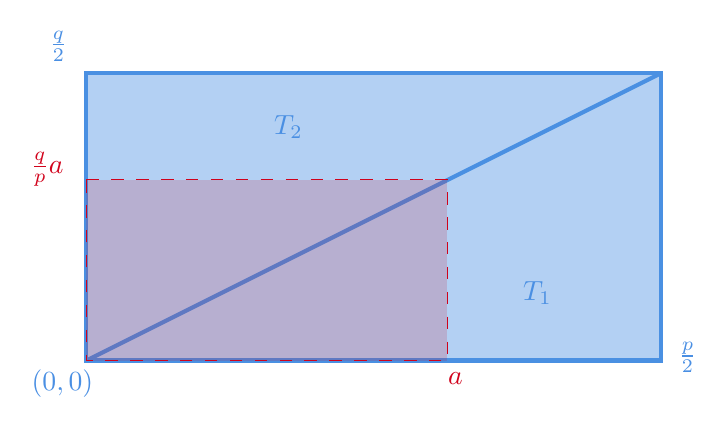
\begin{tikzpicture}[x=0.75pt,y=0.75pt,yscale=-1,xscale=1]
	%uncomment if require: \path (0,300); %set diagram left start at 0, and has height of 300
	%Shape: Rectangle [id:dp5159399739070081] 
	\draw  [color={rgb, 255:red, 74; green, 144; blue, 226 }  ,draw opacity=1 ][fill={rgb, 255:red, 74; green, 144; blue, 226 }  ,fill opacity=0.42 ][line width=1.5]  (181,61) -- (458,61) -- (458,199.5) -- (181,199.5) -- cycle ;
	%Straight Lines [id:da47338369224995747] 
	\draw [color={rgb, 255:red, 74; green, 144; blue, 226 }  ,draw opacity=1 ][line width=1.5]    (181,199.5) -- (458,61) ;
	%Shape: Rectangle [id:dp8995483750887759] 
	\draw  [color={rgb, 255:red, 208; green, 2; blue, 27 }  ,draw opacity=1 ][fill={rgb, 255:red, 208; green, 2; blue, 27 }  ,fill opacity=0.16 ][dash pattern={on 4.5pt off 4.5pt}] (181,112.4) -- (355,112.4) -- (355,199.5) -- (181,199.5) -- cycle ;
	
	% Text Node
	\draw (153.4,202.6) node [anchor=north west][inner sep=0.75pt]    {$\textcolor[rgb]{0.29,0.56,0.89}{( 0,0)}$};
	% Text Node
	\draw (162,39.4) node [anchor=north west][inner sep=0.75pt]    {$\textcolor[rgb]{0.29,0.56,0.89}{\frac{q}{2}}$};
	% Text Node
	\draw (465,189.4) node [anchor=north west][inner sep=0.75pt]    {$\textcolor[rgb]{0.29,0.56,0.89}{\frac{p}{2}}$};
	% Text Node
	\draw (354,204) node [anchor=north west][inner sep=0.75pt]    {$\textcolor[rgb]{0.82,0.01,0.11}{a}$};
	% Text Node
	\draw (153,98) node [anchor=north west][inner sep=0.75pt]    {$\textcolor[rgb]{0.82,0.01,0.11}{\frac{q}{p}}\textcolor[rgb]{0.82,0.01,0.11}{a}$};
	% Text Node
	\draw (390.2,160.2) node [anchor=north west][inner sep=0.75pt]    {$\textcolor[rgb]{0.29,0.56,0.89}{T_{1}}$};
	% Text Node
	\draw (270.2,80.2) node [anchor=north west][inner sep=0.75pt]    {$\textcolor[rgb]{0.29,0.56,0.89}{T_{2}}$};
	\end{tikzpicture}
	\end{equation*}
		Il numero di punti (appartenenti al reticolo intero) interni al rettangolo può essere calcolato facilmente,
	\begin{equation*}
	N=\frac{p-1}{2}\frac{q-1}{2}
	\end{equation*}
	ma possiamo calcolarlo in un altro modo. Su $D$ diagonale non esistono punti interi, infatti la retta ha equazione $y=\frac{q}{p}x$ e se un punto $(a,b)$ vi appartiene allora $bp=qa$, il che vuol dire $p\mid qa$ e questo è impossibile per $a\leq\frac{p}{2}$ - quindi nel rettangolo. Divido il rettangolo in due triangoli $T_1$ e $T_2$, $N$ è ovviamente la somma dei numeri di punti interi nei due triangoli. \\ Per il primo triangolo i punti interi di ascissa $a$ sono
	\begin{equation*}
	\left(a,1\right),\left(a,2\right),\dots,\left(a,\left[\frac{qa}{p}\right]\right)
	\end{equation*}
	In $T_1$ allora ho $\sum_{a=1}^{\frac{p-1}{2}}\left[\frac{qa}{p}\right]$ punti interi, ed analogamente in $T_2$ ne ho $\sum_{a=1}^{\frac{q-1}{2}}\left[\frac{pa}{q}\right]$.
	\begin{equation*}
	N=\sum_{a=1}^{\frac{p-1}{2}}\left[\frac{qa}{p}\right]+\sum_{a=1}^{\frac{q-1}{2}}\left[\frac{pa}{q}\right]
	\end{equation*}
	\begin{align*}
	(-1)^N
	&=(-1)^{\frac{p-1}{2}\frac{q-1}{2}}\\
	&=(-1)^{\sum_{a=1}^{\frac{p-1}{2}}\left[\frac{qa}{p}\right]}(-1)^{\sum_{a=1}^{\frac{q-1}{2}}\left[\frac{pa}{q}\right]}\\
	&=\leg{q}{p}\leg{p}{q}
	\end{align*}
	dove nell'ultimo passaggio ho usato la prima formula dimostrata.   
\end{proof}




\part{Teoria algebrica dei numeri}
\chapter{Introduzione}
\section{Anelli di polinomi}
\subsection{Costruzione}



\label{lezione14}
Sia $A$ un anello commutativo con unità, sia $A[x]$ l'insieme dei polinomi a coefficienti in $A$: si vede facilmente che $\left(A[x],+,\cdot\right)$ è un anello commutativo con unità. In particolare valgono i risultati:
\begin{itemize}
	\item $A$ è un sottoanello di $A[x]$
	\item $A[x]$ è un dominio di integrità se e solo se lo è anche $A$
	\item gli elementi invertibili di $A[x]$ sono tutti e soli gli elementi invertibili dell'anello \enquote{di base} $A$\footnote{Se supponessimo che $A$ non sia un dominio di integrità questo non è più vero. Prendiamo per esempio $A = \mathbb{Z}/4\mathbb{Z}$ e allora il polinomio $2x+3$ è invertibile: $(2x+3)(2x+3) = 4x^2 + (12)x + 9 \equiv 1 \mod \mathbb{Z}/4\mathbb{Z}\left[x\right]$}
\end{itemize}
\begin{definizione}[Campo]
	Sia $(K,+,\cdot)$ un anello commutativo con unità. Se ogni elemento non-nullo ha inverso in $K$ rispetto a $\cdot$, allora si dice \textbf{campo}.
\end{definizione}
\begin{osservazione}[Divisione euclidea per polinomi]
	In particolare se $\mathbb{F}$ è un campo nell'anello $\mathbb{F}[x]$ possiamo costruire la divisione euclidea. Infatti dati $f$ e $g$ in $\mathbb{F}[x]$ con $g$ non nullo, esistono due unici polinomi $q,r$ a coefficienti in $\mathbb{F}$ tali che 
	\begin{equation*}
	f(x)=q(x)g(x)+r(x)
	\end{equation*}
	con $\deg(r)<\deg(g)$ oppure $r=0$. Questo si può vedere facilmente dalla teoria precedente.
\end{osservazione}
\begin{esercizio}
	In $\mathbb{Z}_5[x]$ si divida $f(x)=x^3+x^2+x-1$ per $g(x)=2x^2+1$.
	\begin{center}
		\begin{tabular}{r|r}
			$x^3+x^2+x-1$ & \multicolumn{1}{l}{$2x^2+1$}  \\ 
			\cline{2-2}
			$x^3+3x$      & \multicolumn{1}{l}{$3x+3$}    \\ 
			\cline{1-1}
			$x^2-2x-1$    &                               \\
			$x^2+3$       &                               \\ 
			\cline{1-1}
			$-2x-4$       &                              
		\end{tabular}
	\end{center}
	Si può verificare che $f(x)=(3x+3)g(x)+(3x+1)$. Siccome lavoro in un campo, sono sicuro che esiste un inverso per ogni suo elemento.
\end{esercizio}
\begin{esercizio}
	Siano $f$ e $g$ in $\mathbb{Z}_5[x]$ i polinomi 
	\begin{equation*}
	f(x)=x^5+2x^3+x^2+4x+3\\
	g(x)=x^5+4x^3+x^2+3x+3
	\end{equation*}
	Costruire il massimo comune divisore e la scrittura di Bezout del massimo comune divisore.\\
	La risoluzione è immediata per algoritmo di divisione euclidea:
	\begin{center}
		\begin{tabular}{r|r}
			$f(x)$ & \multicolumn{1}{l}{$g(x)$}  \\ 
			\cline{2-2}
			$x^5+4x^3+x^2+3x+3$      & \multicolumn{1}{l}{$1$}    \\ 
			\cline{1-1}
			$5x^3+x$    &                              
		\end{tabular}
	\end{center}
	quindi $f(x) = g(x) + 5x^3+x$. Da cui 
	\begin{center}
		\begin{tabular}{r|r}
			$g(x)$ & \multicolumn{1}{l}{$5x^3+x$}  \\ 
			\cline{2-2}
			$x^5+3x^3$      & \multicolumn{1}{l}{$3x^2+3$}    \\ 
			\cline{1-1}
			$x^3+x^2+3x+3$    &  \\
			$x^3+3x$ & \\
			\cline{1-1} 
			$x^2+3$ &                      
		\end{tabular}
	\end{center}
	per cui $g(x) = (3x^2+3)(5x^3+x) + x^2+3$ ed osserviamo infine che $5x^3+x = (5x)x^2+3$, 
	segue che $\MCD(f(x),g(x)) = x^2+3$.\\
	Ora dobbiamo trovare i coefficienti per l'identità di Bezout. Prendiamo in considerazione 
	le seguenti equazioni 
	\begin{equation*}
		\begin{array}{l}
			f(x)= g(x) + 5x^3+x  \\
			g(x)= (3x^2+3)(5x^3+x) + (x^2+3) 
		\end{array}
	\end{equation*}
	allora è equivalente al seguente sistema
	\begin{equation*}
		\arraycolsep=1.4pt
		\begin{array}{rl}
			(3x^2+3)(f(x)-g(x)) &= (3x^2+3)(5x^3+x)  \\
			g(x) - (x^2+3) &= (3x^2+3)(5x^3+x)  
		\end{array}
	\end{equation*}
	sostituendo il termine di destra della prima equazione con quanto trovato nella seconda, 
	si ottiene 
	\begin{equation*}
		(4x^2+4)f(x) + (3x^2+4)g(x) = x^2 + 3
	\end{equation*}
	%todo: controlla calcoli, non sono sicuro
\end{esercizio}
\begin{teorema}[di Ruffini]
	Sia $\mathbb{F}$ un campo, $f\in\mathbb{F}[x]$. $\alpha$ è radice di $f$ se e solo se $x-\alpha$ divide $f(x)$.
\end{teorema}
\begin{proof}
	Se $\alpha$ è una radice di $f$ posso dividere $f$ per $(x-\alpha)$:
	\begin{equation*}
	f(x)=q(x)(x-\alpha)+r
	\end{equation*}
	\begin{equation*}
	f(\alpha)=q(\alpha)(\alpha-\alpha)+r=0
	\end{equation*}
	ed ottengo $r=0$. Per l'altro verso invece basta notare che se $x-\alpha$ divide $f$ posso scrivere
	\begin{equation*}
	f(x)=q(x)(x-\alpha)
	\end{equation*}
	e palesemente $f(\alpha)=0$.
\end{proof}
\begin{osservazione}
	Se $f(x)$ ha una sola radice in $\mathbb{F}$, allora $f$ è irriducibile in $\mathbb{F}[x]$. Se non ha radici in $\mathbb{F}$ non è detto che sia irriducibile, ad esempio posso prendere in $\mathbb{R}[x]$ il polinomio
	\begin{equation*}
	x^4+3x^2+2=(x^2+1)(x^2+2)
	\end{equation*}
\end{osservazione}




\subsection{Quozienti in anelli di polinomi}
\begin{lemma}
	Siano $F$ un campo ed $F[x]$ l'anello dei polinomi su $F$, allora $F[x]$ è un PID.
\end{lemma}
\begin{proof}
	Sicuramente $F[x]$ è euclideo perché posso effettuare la divisione euclidea, basta usare come funzione il grado. In particolare, essendo un dominio euclideo, è anche un PID; questo per le caratterizzazioni viste nei capitoli precedenti.
\end{proof}
\begin{osservazione}[Costruire quozienti con i polinomi]
	Possiamo caratterizzare i quozienti in anelli di polinomi partendo da un campo $\mathbb{F}$, e quindi dal suo anello di polinomi $\mathbb{F}[x]$. L'anello quoziente ha forma 
	\begin{equation*}
	\sfrac{\mathbb{F}[x]}{I}
	\end{equation*}
	con $I$ ideale di $\mathbb{F}[x]$. Tutti gli ideali di $\mathbb{F}[x]$ sono principali, ovvero nella forma $I=(f)$ per un polinomio $f\in\mathbb{F}[x]$. Prima di tutto possiamo caratterizzare le classi laterali uguali; $(f)+a$ ed $(f)+b$ lo sono se e solo se 
	\begin{equation*}
	a-b\in(f)
	\end{equation*}
	ovvero per $a-b=kf$ multiplo di $f$. In modo equivalente possiamo dire che $a(x)$ e $b(x)$ sono equivalenti rispetto al quoziente per $(f)$ se e solo se
	\begin{equation*}
	a(x)-b(x)=k(x)f(x)
	\end{equation*}
	Risulta evidente che posso costruire le classi di resto in modo esattamente analogo al caso dei numeri interi.
\end{osservazione}
\begin{proposizione}
	Sia $\mathbb{F}$ un campo, se $p\in\mathbb{F}[x]$ è irriducibile allora 
	\begin{equation*}
	\sfrac{\mathbb{F}[x]}{(p)}
	\end{equation*}
	è un campo.
\end{proposizione}
\begin{proof}
	Sicuramente è un anello commutativo con identità, è abbastanza evidente; vediamo solo che ogni elemento non nullo ha un inverso. Sia $(p)+a$ un elemento di $\sfrac{\mathbb{F}[x]}{(p)}$ tale che $a$ non appartenga all'ideale generato da $p$ (questo vuol dire che $p$ non divide $a$). La nostra scelta è motivata, infatti $(p)+a=(p)$ se e solo se $a-0\in(p)$: in questo caso $a \equiv 0 \mod (p)$ è un elemento nullo, non di nostro interesse. Allora il massimo comune divisore tra $p$ ed $a$ è 1, e per divisione euclidea posso scrivere 
	\begin{equation*}
	1=r(x)a(x)+s(x)p(x)
	\end{equation*}
	per certi $r,s$ polinomi su $\mathbb{F}$. Questo vuol dire che 
	\begin{equation*}
	(p)+1=(p)+ra+sp=\left((p)+r\right)\left((p)+a\right)
	\end{equation*}
	ed ho appena trovato l'inverso di $(p)+a$, perché $(p)+1$ è l'identità moltiplicativa. \\ \\ Si noti che al solito stiamo scrivendo $(p)+a$ evitando di indicare che si tratta di una classe di equivalenza, come sempre accade nell'aritmetica modulare.
\end{proof}
\begin{teorema}[Teorema fondamentale dell'algebra]
	In $\mathbb{C}[x]$, ogni polinomio di grado almeno 1 ha una radice in $\mathbb{C}$. In particolare, per teorema di Ruffini e per la caratterizzazione vista, sono irriducibili in $\mathbb{C}[x]$ solo i polinomi di grado 1.
\end{teorema}
\begin{corollario}
	Un polinomio di grado $n$ su $\mathbb{C}[x]$ ha $n$ radici in $\mathbb{C}$.
\end{corollario}
\begin{teorema}
	In $\mathbb{R}[x]$, un polinomio è irriducibile se e solo se
	\begin{enumerate}
		\item è di primo grado
		\item oppure è di secondo grado con discriminante negativo
	\end{enumerate}
\end{teorema}
\begin{teorema}[di Gauss]
	\label{gauss_pol}
	Sia $f(x)\in\mathbb{Z}[x]$, se $f$ si fattorizza nel prodotto di due polinomi in $\mathbb{Q}[x]$ allora si fattorizza anche nel prodotto di due polinomi in $\mathbb{Z}[x]$.
\end{teorema}
\begin{teorema}
	Sia $f(x)=a_nx^n+\dots+a_1x+a_0\in\mathbb{Z}[x]$ con $a_n\neq0$, se $f$ ha radici in $\mathbb{Q}[x]$ allora sono nella forma $\frac{p}{q}$ dove $p$ divide $a_0$ e $q$ divide $a_n$, $p$ e $q$ coprimi.
\end{teorema}
\begin{teorema}[Criterio di Eisenstein]
	Sia dato il polinomio
	\begin{equation*}
	f(x)= x^n+ a_{n-1}x^{n-1}\dots+a_1x+a_0\in\mathbb{Z}[x]
	\end{equation*}
	se esiste un $p$ primo tale che $p$ divide $a_0,a_1,\dots,a_{n-1}$ e $p^2$ non divide $a_0$, allora $f$ è irriducibile in $\mathbb{Q}[x]$. \\ In particolare è irriducibile anche in $\mathbb{Z}[x]$.
\end{teorema}
\begin{esempio}
	Consideriamo il polinomio $x^2-2$ in $\mathbb{Q}[x]$, tale polinomio è irriducibile, quindi per le caratterizzazioni viste $\mathbb{F}=\sfrac{\mathbb{Q}[x]}{(x^2-2)}$ è un campo. \\ Due polinomi in $\mathbb{Q}[x]$ sono equivalenti in $\mathbb{F}$ se hanno lo stesso resto mediante la divisione per $x^2-2$, quindi tutti i polinomi del campo originale sono rappresentati nel quoziente da polinomi di grado 1. Consideriamo ad esempio i due polinomi in $\mathbb{Q}[x]$
	\begin{equation*}
	a(x)=x^3+2x+1, \quad\ b(x)=x^2-2x-3 
	\end{equation*}
	Possiamo verificare facilmente che 
	\begin{equation*}
	a\equiv4x+1\Mod (x^2-2)
	\end{equation*}
	\begin{equation*}
	b\equiv-2x-1\Mod (x^2-2)
	\end{equation*}
	\begin{equation*}
	ab\equiv-6x-17\Mod (x^2-2)
	\end{equation*}
	Consideriamo ora $\mathbb{Q}[\sqrt{2}]=\left\{a+b\sqrt{2} \, \mid \, a,b\in\mathbb{Q}\right\}$. Si può dimostrare che è un campo rispetto alle solite operazioni sui reali: difatti è palesemente un anello commutativo con unità, ed ogni elemento $a+b\sqrt{2}$ ha inverso moltiplicativo $\frac{a}{c}-\frac{b}{c}\sqrt{2}$ dove $c=a^2-2b^2$ (è la norma). Allora definiamo la mappa
	\begin{align*}
	\varphi:\mathbb{Q}[x]&\longrightarrow\mathbb{Q}[\sqrt{2}]\\
	f(x)&\longmapsto f(\sqrt{2})
	\end{align*}
	Notiamo che verifica le seguenti proprietà:
	\begin{enumerate}
		\item è un morfismo
		\item ha come immagine $\mathbb{Q}[\sqrt{2}]$, è suriettiva
		\item $\varphi\left(a+bx\right)=a+b\sqrt{2}$
		\item il suo nucleo è l'ideale generato da $x^2-2$, questo perché tutti i polinomi in $\mathbb{Q}[x]$ che hanno $\sqrt{2}$ come radici sono divisibili per $x^2-2$; segue da un teorema che non vedremo \footnote{Sia $f$ in $F[x]$ il polinomio minimo di $\alpha$, $g\in F[x]$ un altro polinomio con radice $\alpha$. Allora $f$ divide $g$.} 
	\end{enumerate}
	Per il primo teorema di isomorfismo tra anelli, ottengo che $\mathbb{F}$ è isomorfo a $\mathbb{Q}[\sqrt{2}]$. In particolare notiamo che 
	\begin{equation*}
	a(x) \mapsto 4\sqrt{2}+1
	\end{equation*}
	\begin{equation*}
	b(x) \mapsto -2\sqrt{2}-1
	\end{equation*}
	ed ovviamente moltiplicarli in $\mathbb{F}$ è equivalente a moltiplicarli in $\mathbb{Q}[\sqrt{2}]$.
	\begin{equation*}
	a(x)b(x) \mapsto -6\sqrt{2}-17
	\end{equation*}
\end{esempio}
\begin{esempio}
	In modo esattamente analogo possiamo vedere che 
	\begin{equation*}
	\sfrac{\mathbb{R}[x]}{(x^2+1)}\simeq\mathbb{R}[i]=\mathbb{C}
	\end{equation*}
	infatti basta prendere il morfismo
	\begin{align*}
	\varphi:\mathbb{R}[x]&\longrightarrow\mathbb{R}[\sqrt{-1}]\\
	f(x)&\longmapsto f(\sqrt{-1})
	\end{align*}
	e mostrare che soddisfa le condizioni del primo teorema di isomorfismo, con nucleo $(x^2+1)$.
\end{esempio}




\section{Campi di numeri}
\subsection{Estensioni di campi}
\label{lezione15}
\begin{definizione}
	Dati $K$ ed $F$ campi, si dice che \textbf{$F$ è estensione di $K$} se $K$ è un sottocampo di $F$, non necessariamente proprio. In simboli scriveremo $F/K$.
\end{definizione}
\begin{definizione}
	Un elemento di $F$ si dice \textbf{algebrico su $K$} se è radice di un polinomio a coefficienti in $K$, in particolare l'estensione $F/K$ si dice \textbf{algebrica} se ogni $\alpha\in F$ è algebrico in $K$. \footnote{Chiaramente tutti gli elementi di $K$ sono algebrici su $K$, basta prendere il polinomio $x-a$ in $K[x]$.}
\end{definizione}
\begin{definizione}
	Sia $F/K$ estensione, $\alpha\in F$.
	\begin{enumerate}
		\item $K(\alpha)$ è definito come il più piccolo campo contenente $K$ ed $\alpha$ (che si dice \textbf{estensione semplice} di $K$).
		\item $K[\alpha]$ è l'insieme di tutte le espressioni polinomiali in $\alpha$ a coefficienti in $K$.
		\begin{equation*}
		K[\alpha]=\left\{\sum a_i\alpha^i \ \mid \ a_i\in\ K\right\}
		\end{equation*}
	\end{enumerate}
\end{definizione}
\begin{proposizione} 
	Sotto le condizioni precedenti, vale
	\begin{equation*}
	K(\alpha)\supset K[\alpha] \supset K
	\end{equation*}
\end{proposizione}
\begin{proposizione}
	Consideriamo il morfismo di anelli 
	\begin{align*}
	\varphi: K[x] &\longrightarrow K[\alpha]\\
	f(x)&\longmapsto f(\alpha)
	\end{align*}
	$\alpha$ è algebrico su $K$ se e solo se $\varphi$ non è iniettivo.
\end{proposizione}
\begin{proof}
	Supponiamo che sia algebrico, allora posso scrivere il nucleo del morfismo come 
	\begin{equation*}
	\ker\varphi = \left\{f\in K[x] \ \mid \ f(\alpha)=0\right\}
	\end{equation*}
	e notiamo che per ipotesi non è banale. \\ Supponiamo invece che il nucleo sia non banale, allora è un ideale proprio di $K[x]$, otteniamo facilmente che $\alpha$ è algebrico su $K$. Infatti è generato da un certo $M$ polinomio monico irriducibile: se fosse $M(x)=p(x)q(x)$ avremmo $M(\alpha)=p(\alpha)q(\alpha)=0$, quindi almeno uno dei due (supponiamo sia $p$) apparterrebbe al nucleo. Quindi $M \mid p$ perché supponiamo che l'ideale è generato da $M$, ma $p\mid M$ perché $M(x) = p(x)q(x)$. Quindi $M = p$, necessariamente $q$ è costante ed $M$ è irriducibile. Allora $M$ è il polinomio minimo cercato.
\end{proof}
\begin{teorema}
	$K(\alpha)=K[\alpha]$ se e solo se $\alpha$ è algebrico su $K$.
\end{teorema}
\begin{proof}
	Supponiamo che $\alpha$ sia algebrico; il morfismo $\varphi$ per quanto appena visto ha $\ker \varphi = (M)$, ma è banalmente surgettivo, quindi per il primo teorema di isomorfismo
	\begin{equation*}
	K[\alpha]\simeq\sfrac{K[x]}{(M)}
	\end{equation*}
	dove $M$ è irriducibile in quanto polinomio minimo di $\alpha$, dunque $K[\alpha]$ è un campo. Questo campo contiene sia $K$ che $\alpha$ quindi $K(\alpha)\subset K[\alpha]$. D'altra parte un generico elemento di $K[\alpha]$ appartiene sicuramente a $K(\alpha)$ per la sua scrittura. \\ \\
	Assumiamo che $K(\alpha)=K[\alpha]$, si noti che anche $\alpha^{-1}$ appartiene a $K(\alpha)=K[\alpha]$. Allora per un certo $n$ e per alcuni certi $a_i$ vale
	\begin{equation*}
	\alpha^{-1}=a_0+\dots+a_n\alpha^n
	\end{equation*}
	Inoltre $\alpha^{-1}\alpha-1=0$ per ovvi motivi, quindi il polinomio definito come
	\begin{equation*}
	f(x)=a_nx^{n+1}+\dots+a_1x+a_0x-1 \ \in K[x]
	\end{equation*}
	è tale che $f(\alpha)=0$.
\end{proof}
\begin{osservazione}[Estensioni finite]
	Se $\alpha$ è algebrico, ogni elemento di $K(\alpha)$ si può scrivere in modo unico come polinomio in $\alpha$ a coefficienti in $K$ (di grado inferiore al grado del polinomio minimo di $\alpha$ su $K$). Infatti se $M$ di grado $n$ è il polinomio minimo di $\alpha$ considero $u\in K[x]$, e l'elemento corrispondente $u(\alpha$). Eseguiamo la divisione euclidea:
	\begin{equation*}
	u(x)=q(x)M(x)+r(x) \ \ \deg(r)<n \ \text{ oppure } r=0
	\end{equation*}
	Si ha $u(\alpha)=r(\alpha)$, quindi ogni elemento di $K(\alpha)=K[\alpha]$ si esprime come 
	\begin{equation*}
	a_0+\dots+a_{n-1}\alpha^{n-1}
	\end{equation*}
	Possiamo quindi dire che la dimensione di $K[\alpha]$ visto come spazio vettoriale su $K$ è $n$ (grado del polinomio minimo). D'altra parte se la dimensione di $K[\alpha]$ su $K$ è un $n$ finito, allora prendendo $n+1$ elementi del tipo
	\begin{equation*}
	a,\alpha,\dots,\alpha^n
	\end{equation*}
	questi sono linearmente dipendenti, in altre parole
	\begin{equation*}
	\lambda_0+\dots+\lambda_n\alpha^n=0
	\end{equation*}
	per certi $\lambda_i\in K$ non-nulli, ovvero $\alpha$ è algebrico su $K$.
	In generale per $F=K(\alpha)$ si scrive 
	\begin{equation*}
	[F:K]=\dim_K F
	\end{equation*}
	e vale che ogni estensione finita della forma $K[\alpha]$ è algebrica. \\ Si noti che nel caso più generale ancora, quindi con $F$ estensione qualunque, una estensione algebrica potrebbe non essere finita. Per esempio l'estensione dei numeri algebrici su $\mathbb{Q}$ è algebrica, ma non è finita. \\ \\ Inoltre se si hanno tre campi $K\subset F\subset E$ vale la seguente formula:
	\begin{equation*}
	[E:K]=[E:F][F:K]
	\end{equation*}
	Si può dimostrare costruendo le basi delle estensioni viste come spazi vettoriali sul rispettivo campo di base dell'estensione, ma questo esula dagli scopi del corso.
\end{osservazione}

% TODO: nel caso si volesse inserire una generalizzazione di questo teorema nel caso di domini e A-algebre, si potrebbe inserire il capitolo 4 del Miles Reid.

\begin{teorema}
	Si consideri un'estensione $E/K$ e sia $F$ l'insieme degli $\alpha\in E$ algebrici su $K$. Allora
	\begin{enumerate}
		\item $F$ è un sottocampo di $E$ e si ha $K\subset F\subset E$
		\item $\alpha\in E$ è algebrico su $F$ (quindi $\alpha\in F$)
		\item se $E$ è algebricamente chiuso (ovvero tutti gli elementi di $E[x]$ hanno radice in $E$) allora anche $F$ è algebricamente chiuso.
	\end{enumerate}
\end{teorema}
\begin{proof}\
	\begin{enumerate}
		\item Si ha subito che $K \subset F$, infatti se $\alpha\in K$ si ha che $x-\alpha \in K[x]$. Sia invece $\alpha\in F$ non-nullo, con
		\begin{equation*}
		a_0+\dots+a_n\alpha^n = 0 \ \ a_i \in K
		\end{equation*}
		Moltiplicando per $(\alpha^{-1})^n$ ottengo che $\alpha^{-1}\in F$, infatti
		\begin{equation*}
		a_n+\dots+a_0\left(\frac{1}{\alpha}\right)^n = 0
		\end{equation*}
		Resta da verificare che se $\alpha$ e $\beta$ appartengono ad $F$, allora anche la loro somma ed il loro prodotto appartengono ad $F$. \\ Siccome $\beta$ è algebrico su $K(\alpha)$ si ha 
		\begin{align*}
		[K(\alpha)(\beta):K]=[K(\alpha,\beta):K(\alpha)][K(\alpha):K]
		\end{align*}
		dove i prodotti a destra sono finiti per ipotesi; allora
		\begin{align*}
		[K(\alpha,\beta):K] < +\infty
		\end{align*}
		quindi $K(\alpha,\beta)$ è una estensione algebrica di $K$ (poiché finita), quindi $\alpha+\beta$ ed $\alpha\beta$ sono algebrici su $K$.
		\item Sia $\alpha$ radice del polinomio
		\begin{equation*}
		a_0+\dots+a_nx^n = 0 \ \ a_i \in F
		\end{equation*}
		L'estensione $K(a_1,\dots,a_n)/K$ è algebrica. Per $p\in K(a_1,\dots,a_n)$, $\alpha$ è algebrico su $K(a_1,\dots,a_n)$, cioè $[K(a_1,\dots,a_n)(\alpha):K(a_1,\dots,a_n)]$ è di grado finito. Inoltre
		\begin{equation*}
		[K(a_1,\dots,a_n)(\alpha):K]=[K(a_1,\dots,a_n)(\alpha):K(a_1,\dots,a_n)][K(a_1,\dots,a_n):K]
		\end{equation*}
		è finito, quindi $\alpha$ è algebrico su $K$. Di conseguenza $\alpha$ appartiene ad $F$.
		\item Sia $p\in F[x]$ di grado maggiore di $1$, se $E$ è algebrico chiuso esiste un $\alpha\in E$ tale che $p(\alpha)=0$. Per il punto 2 otteniamo $\alpha\in F$ ed algebrico, quindi ogni polinomio a coefficienti in $F$ ha radice in $F$.
	\end{enumerate}
\end{proof}
\begin{definizione}[Campi di numeri]
	Un \textbf{campo di numeri} (o campo numerico) è un'estensione finita di $\mathbb{Q}$.
\end{definizione}




\section{Equazioni diofantine}
\label{lezione16}
\epigraph{\textit{\enquote{Cubum autem in duos cubos, aut quadratoquadratum in duos quadratoquadratos et generaliter nullam in infinitum ultra quadratum potestatem in duos eiusdem nomines fas est dividere cuius rei demonstrationsm mirabile sane detexi. Hanc marginis exiguitas non caperet.}}}{Fermat, commentando su un margine \enquote{\textsc{Arithmetica}}}
Nel 300 d.C. Diofanto di Alessandria scrive \textit{Arithmetica}, che introduce il loro studio. Le equazioni diofantine (o diofantee) sono equazioni ad una o più incognite di cui si ricercano le soluzioni intere - ed a volte si cerca addirittura di capire se siano finite. Alcune famose equazioni diofantine, legate ad altrettanti famosi problemi matematici, sono
\begin{itemize}
	\item $x^2+y^2=z^2$, terne pitagoriche
	\item $x^2+y^2=n$, teorema dei due quadrati
	\item $x^2-Dy^2=1$, equazione di Pell
	\item $x^n+y^n=z^n$ ($n\geq3$), ultimo teorema di Fermat
\end{itemize}
Come possiamo vedere il loro studio è strettamente legato alla teoria dei numeri, in particolare allo studio delle {proprietà dei numeri algebrici}. \\ Potremmo dire che la teoria dei numeri è nata da problemi pratici (il teorema di Pitagora) e dallo studio dei numeri interi.
\subsection{Alcune equazioni diofantine}
\begin{teorema}
	L'unica soluzione intera dell'equazione diofantea
	\begin{equation*}
	x^3=y^2+1
	\end{equation*}
	è $x=1$, $y=0$.
\end{teorema}
\begin{proof}
	Siano $x,y$ le soluzioni intere dell'equazione diofantina. Se $x$ fosse pari avremmo 
	\begin{equation*}
	y^2\equiv x^3-1\equiv -1 \Mod 4
	\end{equation*}
	 e quindi $x$ deve essere dispari, perché $-1$ non è un quadrato in modulo 4. Lavoriamo in $\mathbb{Z}[i]$: abbiamo 
	 \begin{equation*}
	 x^3=(y+i)(y-i)
	 \end{equation*}
	 Un divisore $m$ comune a $y-i, y+i$ divide anche $2i$, e quindi $2$ dato che $i$ è un'unità; infatti se $m \mid y-i$ e $m \mid y+i$ allora $m \mid y+i-(y-i) = 2i$. Allora $m$ divide $x^3$ dispari ed $m$ divide $2$, ma $x^3$ e $2$ sono coprimi, quindi sono coprimi anche $y+i$ ed $y-i$. Siccome sono in un dominio a fattorizzazione unica e $(y+i)(y-i)$ è un cubo, allora lo sono anche $y+i$ ed $y-i$ per lemma successivo. Ottengo che $y+i$ ha forma $(a+bi)^3$ per certi $a$ e $b$ interi, da cui 
	 \begin{equation*}
	 \begin{cases}
	 y=a^3-3ab^2\\1=3a^2b-b^3
	 \end{cases}
	 \end{equation*}
	 Abbiamo quindi $b(3a^2-b^2)=1$, e per proprietà elementare del prodotto otteniamo i due casi
	 \begin{equation*}
	 \begin{cases}
	 &b=1 \\
	 &3a^2-1=1\implies 3a^2=2
	 \end{cases} \ \ \ \ \ 
	 \begin{cases}
	 &b=-1\\
	 &3a^2-1=-1 \implies a=0
	 \end{cases}
	 \end{equation*}
	 Siccome cerchiamo soluzioni intere il primo caso è da scartare, ma il secondo ci permette di ottenere 
	 \begin{equation*}
	 y-i=(0-i)^3\implies y=0
	 \end{equation*}
	 \begin{equation*}
	 x=(y-i)(y+i)=(-1)(i)=1
	 \end{equation*}
\end{proof}
\begin{lemma}
	Sia $R$ un UFD, $a,b\in R$ coprimi. Sia $x\in R$ tale che $ab=x^n$, $n\in\mathbb{N}$. Allora $a$ e $b$ sono potenze $n$-esime.
\end{lemma}
\begin{proof}
	Ovvio, $x=p_1^{e_1}\dots p_r^{e_r}$ e $x^n=p_1^{e_1n}\dots p_r^{e_rn}$
\end{proof}
\begin{osservazione}
	Il lemma vale a meno di unità, consideriamo ad esempio
	\begin{align*}
	900=30^2&=(6^2)(5^2)=(36)(25)\\
	&=(-36)(-25)
	\end{align*}
	Si vede che nella prima riga otteniamo un prodotto di due quadrati, nella seconda invece no.
\end{osservazione}
\begin{esercizio}
	Si verifichi che in $\mathbb{Z}[i]$ tutte le unità sono dei cubi. \\ \\ Si può dimostrare in modo diretto, oppure osservando che le unità formano un gruppo ciclico di ordine 4.
	Infatti tutte le unità di $\mathbb{Z}[i]$ sono $1,i,-1,-i$ e si può vedere che $i$ genera tutto il gruppo, infatti $i^2 = -1$, $i^3 = -i$ e $i^4 = 1$ e quindi $U(\mathbb{Z}[i]) \simeq (\mathbb{Z}_4, +)$.
\end{esercizio}




\chapter{Campi numerici}
I campi numerici svolgono un ruolo fondamentale nella teoria algebrica dei numeri. Lo scopo di questo corso non è lavorare sui problemi complessi della teoria algebrica dei numeri, ma fornire gli strumenti necessari per approcciarli; iniziamo quindi a studiare gli spazi in cui si svolgerà gran parte del nostro lavoro. Li abbiamo già incontrati in precedenza, ma ora diventeranno predominanti. \\ \\
Ricordiamo che i campi di numeri sono estensioni finite di $\mathbb{Q}$, ad esempio sono campi numerici
\begin{itemize}
	\item $\mathbb{Q}(i)$, di grado $[\mathbb{Q}(i):\mathbb{Q}]=2$
	\item $\mathbb{Q}(\sqrt{2})$, di grado $[\mathbb{Q}(\sqrt{2}):\mathbb{Q}]=2$
	\item $\mathbb{Q}(\sqrt[4]{2})$, di grado $[\mathbb{Q}(\sqrt[4]{2}):\mathbb{Q}]=4$
	\item $\mathbb{Q}(\sqrt[3]{3},\sqrt{7})$, di grado $[\mathbb{Q}(\sqrt[3]{3},\sqrt{7}):\mathbb{Q}]=6$
\end{itemize}




\section{Introduzione ai campi numerici}
\subsection{Caratterizzazioni dei campi di numeri}
\begin{teorema}[Teorema dell'elemento primitivo]
	Sia $F$ un campo numerico. Allora esiste un $\theta$ elemento di $F$ tale che $F=\mathbb{Q}(\theta)$, ovvero $F$ è sempre un'estensione semplice.
\end{teorema}
\begin{proof}
	Consideriamo il caso in cui $F=\mathbb{Q}(\alpha,\beta)$; sarà sufficiente, perché da questo potrò procedere per induzione su ogni campo di numeri. La dimostrazione è costruttiva, quindi ci fornirà una procedura per costruire il polinomio minimo di $\theta$. \\ \\ 
	Cerchiamo un $\theta$ tale che $\mathbb{Q}(\theta)=\mathbb{Q}(\alpha,\beta)$. \\ Sia $f\in\mathbb{Q}[x]$ il polinomio minimo di $\alpha$ di grado $n$, siano $\alpha_1,\dots,\alpha_n$ le sue radici distinte nel campo complesso. Sia analogamente $g\in\mathbb{Q}[x]$ il polinomio minimo di $\beta$ di grado $m$ e siano $\beta_1,\dots,\beta_m$ le sue radici complesse distinte. Prendiamo queste radici in modo che $\alpha_1=\alpha$ e $\beta_1=\beta$.\\ Prendiamo un $\lambda\in\mathbb{Q}$ tale che 
	\begin{equation*}
	\lambda\neq\frac{\alpha_i-\alpha}{\beta-\beta_j}
	\end{equation*}
	ovvero tali che $\alpha+\lambda\beta\neq\alpha_i+\lambda\beta_j$, con $1\leq i\leq n$ e $1\leq j\leq m$ . Allora fisso il valore $\theta=\alpha+\lambda\beta$ e considero i polinomi
	\begin{equation*}
	h(x)=f\left(\theta-\lambda x\right)\in\mathbb{Q}(\theta)[x]
	\end{equation*}
	\begin{equation*}
	g(x)\in\mathbb{Q}(\theta)[x]
	\end{equation*}
	con $h(\beta)=g(\beta)=0$. Le radici di $h$ sono 
	\begin{equation*}
	\beta, \frac{\theta-\alpha_2}{\lambda},\dots,\frac{\theta-\alpha_n}{\lambda}
	\end{equation*}
	e le radici di $g$ sono
	\begin{equation*}
	\beta, \beta_2, \dots, \beta_m
	\end{equation*}
	con $b_j\neq\frac{\theta-\alpha_i}{\lambda}$, ovvero $\MCD(h,g)=x-\beta$. Siccome $g$ ed $h$ sono polinomi minimi sono anche monici, e vale anche che $x-\beta\in\mathbb{Q}(\theta)[x]$. Questo equivale a $\beta\in\mathbb{Q}(\theta)$. In modo analogo posso ottenere $\alpha\in\mathbb{Q}(\theta)$.
	Allora ho dimostrato la tesi intermedia: $\mathbb{Q}(\theta) = \mathbb{Q}(\alpha,\beta)$. \\ \\ 
	Per dimostrare la tesi procedo per induzione sul numero di elementi primitivi che costituiscono la mia estensione.
\end{proof}
\begin{esempio}
	$\mathbb{Q}(\sqrt[3]{3}+\sqrt{7})=\mathbb{Q}(\sqrt[3]{3},\sqrt{7})$ \\ \\ 
	Il polinomio minimo di $\sqrt[3]{3}$ infatti è $x^3-3$ che ha soluzioni complesse 
	\begin{equation*}
	\sqrt[3]{3}, \omega \sqrt[3]{3}, \omega^2 \sqrt[3]{3}
	\end{equation*}
	(dove $\omega$ è radice terza primitiva dell'unità). Invece il polinomio minimo di $\sqrt{7}$ è $x^2-7$ che ha soluzioni complesse $\sqrt{7}, -\sqrt{7}$. Nello spirito della dimostrazione, possiamo prendere $\lambda=1$ e quindi $\theta=\sqrt[3]{3}+\sqrt{7}$ il cui polinomio minimo è
	\begin{align*}
	\left(x-(\sqrt[3]{3}+\sqrt{7})\right)&\left(x-(\sqrt[3]{3}-\sqrt{7})\right)\left(x-(\omega\sqrt[3]{3}+\sqrt{7})\right)\dots\\
	&\ \ \ \dots \left(x-(\omega^2\sqrt[3]{3}+\sqrt{7})\right)\left(x-(\omega^2\sqrt[3]{3}-\sqrt{7})\right)
	\end{align*}
	che è un polinomio di grado 6. Allora anche il grado dell'estensione $\mathbb{Q}(\sqrt[3]{3},\sqrt{7})$ su $\mathbb{Q}$ è 6.
\end{esempio}




\subsection{Il polinomio ciclotomico $n$-esimo}
\begin{definizione}
	Diciamo \textbf{$n$-esimo polinomio ciclotomico} $\Phi_n(x)$ il polinomio minimo delle radici primitive $n$-esime primitive dell'unità.
	\begin{equation*}
	\Phi_n(x)=\prod_{k}(x-\omega_k)\in\mathbb{Z}[x]
	\end{equation*}
	dove $k$ è indicizzato da $0\leq k\leq n-1, (k,n)=1$. Il grado del polinomio ciclotomico $\Phi_n(x)$ è $\varphi(n)$.
\end{definizione}
\begin{definizione}[Campi ciclotomici]
	I campi ciclotomici sono campi numerici generati da una radice primitiva $n$-esima dell'unità, hanno forma $\mathbb{Q}(\omega_k)$ - dove $\omega_k$ è la suddetta radice primitiva. Per la teoria svolta, possiamo anche caratterizzarli come
	\begin{equation*}
	\mathbb{Q}(\omega_k)\simeq\sfrac{\mathbb{Q}[x]}{(\Phi_n(x))}
	\end{equation*}
	Il grado di $\mathbb{Q}(\omega_k)$ su $\mathbb{Q}$ è $\varphi(n)$.
\end{definizione}
\begin{teorema}
	Il polinomio ciclotomico $\Phi_n(x)$ è irriducibile in $\mathbb{Q}[x]$.
\end{teorema}
\begin{proof}
	Sia $g\in\mathbb{Q}[x]$ un fattore irriducibile monico di $\Phi_n(x)$, scriviamo per teorema di Gauss \ref{gauss_pol}
	\begin{equation*}
	x^n-1=g(x)h(x)
	\end{equation*}
	con $g,h\in\mathbb{Z}[x]$. Sia $\alpha$ radice complessa di $g$, quindi è radice anche del polinomio $x^n-1$. Sia $p$ primo che non divide $n$, allora $\alpha^p$ è radice di $x^n-1$: infatti se $\alpha^n-1 = 0$
	\begin{equation*}
	\alpha^n = 1\implies \alpha^{pn} - 1 = (\alpha^n)^p - 1 = 0
	\end{equation*}
	Abbiamo due casi:
	\begin{itemize} 
		\item[($g(\alpha^p)\neq0$)] allora $h(\alpha^p)=0$ e $g(x)$ divide $h(x^p)$, questo implica che $g(x)$ divide $h(x)^p$ in $\mathbb{Z}_p[x]$. Sia $f$ un divisore irriducibile di $g$ in $\mathbb{Z}_p[x]$, allora $f$ divide $g$ ed $h$ modulo $p$, ovvero $x^n-1$ ha uno zero doppio modulo $p$; ma non è possibile, perché $nx^{n-1}$ non ha zeri in comune con $x^n-1$ dato che $n\not\equiv0\Mod p$. Concludiamo che il caso $g(\alpha^p)\neq0$ è falso.
		\item[($g(\alpha^p)=0$)] di conseguenza possiamo dire che per ogni $p$ che non divide $n$, per ogni $\alpha$ complesso radice di $g$, anche $g(\alpha^p)=0$; ovvero $g(\alpha^k)=0$ per ogni $k$ coprimo con $n$. Questo dimostra che $\Phi_n$ e $g$ hanno gli stessi zeri, ovvero $\Phi_n(x)=g(x)$. In particolare è irriducibile.
	\end{itemize}
\end{proof}




\section{Campi algebrici}
\subsection{Interi algebrici}
\label{lezione17}
Dato un generico $a\in\mathbb{Q}$, come capisco se $a\in\mathbb{Z}$?
\begin{proposizione}
	Sia $a\in\mathbb{Q}$, questo è intero se e solo se è radice di un polinomio monico in $\mathbb{Z}[x]$.
\end{proposizione}
\begin{proof}
	Se $a$ è intero, allora prendo il polinomio $f(x)=x-a\in\mathbb{Z}[x]$. Se invece è radice di un polinomio monico nella forma
	\begin{equation*}
	f(x)=x^n+a_{n-1}x^{n-1}+\dots+a_0
	\end{equation*}
	Allora $a=\frac{p}{q}$, con $p$ divisore di $a_0$ e $q$ divisore di 1.
\end{proof}
\begin{definizione}
	Un $z\in\mathbb{C}$ si dice \textbf{intero algebrico} se è radice di un polinomio monico a coefficienti interi.
\end{definizione}
\begin{osservazione}
	Diciamo $\mathcal{O}$ l'insieme degli interi algebrici e $\overline{\mathbb{Q}}$ la chiusura algebrica di $\mathbb{Q}$, si può osservare che $\sfrac{\overline{\mathbb{Q}}}{\mathbb{Q}}$ è un'estensione algebrica infinita. Questo perché per ogni $n\geq1$ esiste un polinomio a coefficienti interi $p$ di grado $n$ irriducibile su $\mathbb{Q}$. Ad esempio possiamo costruire $x^n+2$ sfruttando il criterio di Eisenstein. \\ D'altro canto $\mathbb{C}$ ed $\mathbb{R}$ sono estensioni di $\mathbb{Q}$, ma non sono estensioni algebriche - ad esempio $\pi$ è trascendente. \\ \\ L'anello $\mathcal{O}$ degli interi algebrici è incluso nella chiusura algebrica di $\mathbb{Q}$.
\end{osservazione}
\begin{definizione}[Anello degli interi]
	Sia $R$ un anello ed $A$ un suo sottoanello, un $r\in R$ si dice essere \textbf{intero su $A$} se esiste un polinomio monico $p$ a coefficienti in $A$ tale che $p(r)=0$. \footnote{Questo mi permette di definire degli \textit{elementi interi} rispetto ad ogni anello.}
\end{definizione}
\begin{definizione}[$A$-modulo]
	Sia $A$ un anello commutativo con unità 1, $(M,+,0)$ un gruppo commutativo. Definisco l'operazione 
	\begin{align*}
	\cdot \ : A\times M &\longrightarrow M\\
	(a,m)&\longmapsto am
	\end{align*}
	in modo che goda delle seguenti proprietà:
	\begin{enumerate}
		\item $(a+b)m=am+bm$
		\item $a(m+n)=(am)+(an)$
		\item $a(bm)=(ab)m$
		\item $1m=m$
	\end{enumerate}
	Allora $M$ si dice essere un \textbf{$A$-modulo}. \\ A tutti gli effetti si tratta della generalizzazione della definizione di spazio vettoriale.
\end{definizione}
\begin{proposizione}
	Sia $R$ un anello ed $A$ un suo sottoanello, dati $r_1,\dots,r_n\in R$ sono equivalenti:
	\begin{enumerate}
		\item gli $r_i$ sono interi su $A$
		\item $A[r_1,\dots,r_n]$ è un $A$-modulo finitamente generato
		\item esiste un anello $B$ che può essere visto come $A$-modulo finitamente generato, ed è tale che $A[r_1,\dots,r_n]\subset B\subset R$
	\end{enumerate}
\end{proposizione}
\begin{proof}\
	\begin{itemize}
		\item[($1\implies 2$)] Se $n=1$, per certi $a_i\in A$ vale 
		\begin{equation*}
		r_1^m+\dots+a_1r_1+a_0=0
		\end{equation*}
		quindi $r_i^k$ per $k\geq m$ si esprime come combinazione lineare di $1,r_1,\dots,r_1^{m-1}$ a coefficienti in $A$. Procedo poi per induzione su $n$: siccome $r_n$ intero su $A$ è intero su 
		\begin{equation*}
			A[r_1,\dots,r_{n-1}]=C
		\end{equation*}
		e $C[r_n]$ è finitamente generato come $C$-modulo, per ipotesi induttiva ottengo che $C$ è finitamente generato come $A$-modulo, quindi anche $C[r_n]$.
		\item[($2\implies 3$)] Immediato.
		\item[($3\implies 1$)] Basta mostrare che ogni $b\in B$ è intero su $A$. Siano $b_1,\dots,b_k$ generatori di $B$, considero $b\cdot b_i \in B$.
		\begin{equation*}
		 b\cdot b_i = \sum_j a_{ij}b_j \implies \sum_j(\delta_{ij}b-a_{ij})b_j=0
		\end{equation*}
		Questo può essere riscritto ponendo $M=(\delta_{ij}b-a_{ij})_{ij}$, quindi come sistema lineare omogeneo:
		\begin{equation*}
		M
		\begin{pmatrix}
		b_1\\ \vdots \\ b_k
		\end{pmatrix}
		=0
		\end{equation*}
		da cui
		\begin{equation*}
		\det(M)\cdot b_j=0
		\end{equation*}
		quindi per combinazione lineare dei $b_j$ ottengo $\det(M)=0$; infatti siccome generano il modulo deve esistere una loro combinazione lineare che dia 1 come risultato.
		Allora $b$ soddisfa un polinomio monico a coefficienti in $A$.
	\end{itemize}
\end{proof}
\begin{corollario}
	L'insieme degli $r\in R$ interi su $A$ è un sottoanello di $R$.
\end{corollario}
\begin{proof}
	Se $x$ ed $y$ sono elementi di $R$ interi su $A$, allora 
	\begin{equation*}
	A[x+y]\subset A[x,y]
	\end{equation*}
	\begin{equation*}
	A[xy]\subset A[x,y]
	\end{equation*}
\end{proof}




\subsection{Il campo delle frazioni}
Dato $R$ dominio di integrità, è possibile costruire il campo delle frazioni su $R$. Il ragionamento è analogo a quello della costruzione dei razionali a partire dagli interi. \\ \\ Iniziamo da una relazione di equivalenza su $R\times R$:
\begin{equation*}
	(a,b)\sim(c,d) \iff ad=bc
\end{equation*}
con $b,d$ non-nulli. 
\begin{proposizione}
	Si tratta di una relazione di equivalenza.
\end{proposizione}
\begin{proof}\
	\begin{itemize}
		\item[(riflessiva)] Ovvio.
		\item[(simmetrica)] Se $(a,b)\sim(c,d)$, questo vuol dire $ad=bc$. Devo ottenere $(c,d)\sim(a,b)$, ovvero $cb=da$, ma anche questo è ovvio.
		\item[(transitiva)] Se $(a,b)\sim(c,d)$ e $(c,d)\sim(e,f)$, ho come ipotesi
		\begin{equation*}
			ad=bc \ \ \ \ cf=de
		\end{equation*}
		e devo ottenere $af=be$, ma è ovvio dopo aver svolto alcuni passaggi banali come
		\begin{equation*}
		ad=bc\implies a(de)(de)^{-1}=bc
		\end{equation*}
	\end{itemize}
\end{proof}
\begin{definizione}
	Il campo $F$ delle frazioni di $R$ è l'insieme delle classi di equivalenza 
	\begin{equation*}
	[a,b]=\left\{(c,d)\in R\times (R\setminus\left\{0\right\}) \ \mid \ (a,b)\sim(c,d)\right\}
	\end{equation*}
	i cui elementi si indicano con la frazione $\frac{a}{b}$, sotto le operazioni
	\begin{equation*}
	[a_1,b_1]+[a_2,b_2]=[a_1+a_2,b_1+b_2]
	\end{equation*}
	\begin{equation*}
	[a_1,b_1][a_2,b_2]=[a_1a_2,b_1b_2]
	\end{equation*}
\end{definizione}
\begin{osservazione}[Immersione di $R$ in $F$]
	La seguente mappa è un morfismo di anelli tra $R$ sottoanello di $F$ - dove $F$ è il campo delle frazioni appena definito - ed il più piccolo campo contenente $R$:
	\begin{align*}
	\Phi:R&\longrightarrow F\\
	a&\longmapsto [a,1]
	\end{align*}
	si tratta dell'immersione di $R$ in $F$.
\end{osservazione}
\begin{proposizione}
	Sia $K$ un campo, 
	\begin{itemize}
		\item se ha caratteristica zero contiene un sottocampo isomorfo a $\mathbb{Q}$
		\item se ha caratteristica $p$ contiene un sottocampo isomorfo a $\mathbb{Z}_p$
	\end{itemize}
\end{proposizione}
\begin{esempio}
	Un caso abbastanza banale è $R=\mathbb{Z}$, che ha come campo delle frazioni $F\simeq\mathbb{Q}$.
\end{esempio}
\begin{teorema}
	L'anello degli interi algebrici $\mathcal{O}$ è un dominio il cui campo delle frazioni è la chiusura algebrica di $\mathbb{Q}$.
\end{teorema}
\begin{proof}
	Sia $F$ il campo delle frazioni di $\mathcal{O}$, sicuramente è contenuto nella chiusura algebrica di $\mathbb{Q}$; questo perché $\overline{\mathbb{Q}}$ contiene $\mathcal{O}$ ed $F$ è per definizione il più piccolo campo contenente $\mathcal{O}$. \\ \\ Mostriamo che $\overline{\mathbb{Q}}$ è contenuto in $F$. Un elemento $z\in\overline{\mathbb{Q}}$ è radice di un polinomio a coefficienti in $\mathbb{Q}$; allora posso determinare un polinomio a coefficienti interi di cui $z$ sia radice:
	\begin{equation*}
	a_nz^n+a_{n-1}z^{n-1}+\dots+a_1z+a_0=0
	\end{equation*}
	da cui moltiplicando per $a_n^{n-1}$ ottengo
	\begin{equation*}
	(a_nz)^n+a_{n-1}(a_nz)^{n-1}+\dots+a_1a_n^{n-2}(a_nz)+a_0a_{n-1}=0
	\end{equation*}
	ovvero $a_nz\in \mathcal{O}$ in quanto radice del polinomio monico in $\mathbb{Z}[x]$
	\begin{equation*}
	x^n+a_{n-1}x^{n-1}+\dots+a_1a_n^{n-1}x+a_0a_{n-1}
	\end{equation*}
	Ma allora $z=\frac{a_nz}{a_n}$ con $a_nz,a_n\in \mathcal{O}$, ovvero $z\in F$.
\end{proof}
\begin{osservazione}
	Proprio come $\mathbb{Z}\subset\mathbb{Q}$, con $\mathbb{Q}$ campo delle frazioni di $\mathbb{Z}$, si ha $\mathcal{O}\subset\overline{\mathbb{Q}}$, con $\overline{\mathbb{Q}}$ campo delle frazioni di $\mathcal{O}$. \\ \\ Dato un campo di numeri $K$ posso inoltre porre 
	\begin{equation*}
	\mathcal{O}_K=K\cap \mathcal{O}
	\end{equation*}
	In questo modo $\mathcal{O}_K$ è un dominio il cui campo delle frazioni è $K$ ed è l'anello degli interi di $K$.
\end{osservazione}
\begin{esempio}
	Alcuni esempi in $\mathbb{Z}$:
	\begin{itemize}
		\item $\sqrt{2}$ è un intero algebrico, è radice di $x^2-2$
		\item $\frac{1}{\sqrt{2}}$ non è un intero algebrico, è radice di $2x^2-1$
		\item $i$ è un intero algebrico, $x^2+1$
		\item $\phi=\frac{1+\sqrt{5}}{2}$ è un intero algebrico, radice di $x^2-x-1$
	\end{itemize}
\end{esempio}
\begin{esempio}
	$\mathbb{Q}[i]$ è un campo numerico di grado 2, contenente l'anello degli interi di Gauss $\mathbb{Z}[i]$. Vogliamo mostrare che questo è proprio l'anello degli interi di $\mathbb{Q}[i]$, in particolare che dato $z=a+bi\in\mathbb{Q}[i]$ questo è un suo intero algebrico se e solo se $a,b\in\mathbb{Z}$. \\ \\
	Se prendo un elemento di $\mathbb{Q}[i]$ i cui $a,b$ appartengono a $\mathbb{Z}$, questo è un intero algebrico, perché è radice del polinomio monico a coefficienti interi
	\begin{equation*}
	\left(x-(a+bi)\right)\left(x-(a-bi)\right)\in\mathbb{Z}[x]
	\end{equation*}
	Per l'altra implicazione invece prendo uno $z\in\mathbb{Q}[i]$ intero algebrico, ovvero $z\in O$. Allora $z\in \mathcal{O}_{\mathbb{Q}[i]}$. Voglio mostrare che $a$ e $b$ sono interi. Prendo $\overline{z}$, che è ancora un intero algebrico per ipotesi; anche $\overline{z}\in \mathcal{O}_{\mathbb{Q}[i]}$. Siccome $\mathcal{O}$ è un anello
	\begin{equation*}
	z+\overline{z}=2a\in \mathcal{O}
	\end{equation*}
	\begin{equation*}
	z+\overline{z}\in \mathcal{O} \cap \mathbb{Q} = \mathbb{Z}
	\end{equation*}
	Facciamo qualcosa di analogo con $-iz$, che appartiene ancora agli interi algebrici. Allora anche $-iz+i\overline{z}$ è un intero algebrico, e 
	\begin{equation*}
	-iz+i\overline{z}=2b \in \mathcal{O}\cap\mathbb{Q}=\mathbb{Z}
	\end{equation*}
	Abbiamo ottenuto che $2a=m$ e $2b=n$ per certi $m$ ed $n$ interi; devo dimostrare che sono pari. \\ $z\cdot\overline{z}\in\mathbb{Q}\cap \mathcal{O} =\mathbb{Z}$, quindi
	\begin{equation*}
	z\cdot\overline{z}=a^2+b^2=\frac{m^2+n^2}{4}\in\mathbb{Z}
	\end{equation*}
	ovvero $m^2+n^2\equiv0\Mod4$; perché siano dei residui quadrati $m^2$ ed $n^2$ devono essere 0 oppure 1 in modulo 4, ma per quanto appena osservato la loro somma deve essere congrua a zero. Necessariamente devono essere entrambi zero, in particolare sono pari. \\ \\ Allora $\mathbb{Z}[i]$, anello degli interi di Gauss, è anello degli interi di $\mathbb{Q}[i]$.
\end{esempio}
\begin{esempio}
	Consideriamo
	\begin{equation*}
	\mathbb{Q}[\sqrt{5}]=\left\{a+b\sqrt{5} \ \mid \ a,b\in\mathbb{Q}\right\}
	\end{equation*}
	un'estensione di grado 2 su $\mathbb{Q}$. Trova il suo anello degli interi. \\ \\
	In questo caso $\mathbb{Z}[\sqrt{5}]$ non è uguale a $\mathcal{O}_{\mathbb{Q}[\sqrt{5}]}$, è solo incluso. Infatti prendo un $a+b\sqrt{5}\in\mathbb{Z}[\sqrt{5}]$, il polinomio monico di cui è radice si calcola facilmente:
	\begin{align*}
	\left(x-(a+b\sqrt{5})\right)\left(x-(a-b\sqrt{5})\right)&=x^2-2ax+a^2-5b^2\in\mathbb{Z}[x]
	\end{align*}
	Tuttavia prendo $\frac{1+3\sqrt{5}}{2}$, questo è un intero algebrico perché ha come polinomio monico $x^2-x-11$ ma non appartiene a $\mathbb{Z}[\sqrt{5}]$
\end{esempio}




\section{Norma, traccia e discriminante}
\label{lezione18}
\subsection{Immersioni in $\mathbb{C}$}
\begin{definizione}
	Sia $F$ un campo numerico, si dice essere una sua \textbf{immersione in $\mathbb{C}$} un morfismo iniettivo 
	\begin{equation*}
	\varphi: F \longmapsto \mathbb{C}
	\end{equation*}
	In particolare l'immersione si dice \textbf{reale} se la sua immagine $\varphi(F)$ è contenuta in $\mathbb{R}$, altrimenti si dice \textbf{complessa}.
\end{definizione}
\begin{osservazione}[Immersioni per elementi primitivi]
	Consideriamo $\mathbb{Q}(\alpha)$, con $\alpha$ elemento primitivo, estensione di grado $n$ su $\mathbb{Q}$. Sia $M_\alpha(x)$ il polinomio minimo di $\alpha$, con radici $\alpha_1,\dots,\alpha_n$ ($\alpha_1=\alpha$). \\ \\ Le immersioni di $\mathbb{Q}(\alpha)$ in $\mathbb{C}$ sono le funzioni definite da 
	\begin{align*}
	\sigma_i:\mathbb{Q}(\alpha)&\longrightarrow \overline{\mathbb{Q}}\\
	\alpha&\longmapsto\alpha_i\\
	k&\longmapsto k \ \ \text{se $k\in\mathbb{Q}$}
	\end{align*}
	Allora possiamo notare che 
	\begin{enumerate}
		\item $M_\alpha(x)=\prod_i\left(x-\sigma_i(\alpha)\right)$ è una forma del suo polinomio minimo
		\item gli $\alpha_2,\dots,\alpha_n$ sono detti \textbf{coniugati di $\alpha$ }
	\end{enumerate}
\end{osservazione}
\begin{osservazione}[Immersioni per elementi non primitivi]
	Proviamo a lavorare su $\beta\in\mathbb{Q}(\alpha)$ elemento non primitivo, abbiamo le relazioni di inclusione 
	\begin{equation*}
	\mathbb{Q}\subset\mathbb{Q}(\beta)\subset\mathbb{Q}(\alpha)
	\end{equation*}
	Sia $m$ il grado di $\mathbb{Q}(\beta)$ su $\mathbb{Q}$, $t$ il grado di $\mathbb{Q}(\alpha)$ su $\mathbb{Q}(\beta)$. 
	\begin{enumerate}
		\item per formula dei gradi vale 
		\begin{align*}
		\left[\mathbb{Q}(\alpha):\mathbb{Q}\right]&=\left[\mathbb{Q}(\alpha):\mathbb{Q}(\beta)\right]\left[\mathbb{Q}(\beta):\mathbb{Q}\right]\\
		&=t\cdot m
		\end{align*}
		\item allora per proprietà delle estensioni vale anche 
		\begin{equation*}
		\left(M_\beta(x)\right)^t=\prod_{i=1}^m\left(x-\sigma_i(\beta)\right)
		\end{equation*}
	\end{enumerate}
	Si noti quindi che se $\alpha$ è primitivo i suoi coniugati sono le radici (distinte) del polinomio minimo, se invece non è primitivo i suoi coniugati sono le radici contate con ripetizione. Lo vedremo in seguito. \\
	Definiamo l'applicazione 
	\begin{align*}
	m_z:\mathbb{Q}(\alpha)&\longrightarrow\mathbb{Q}(\alpha)\\
	x&\longmapsto zx
	\end{align*}
	questo è un endomorfismo di $\mathbb{Q}(\alpha)$ visto come $\mathbb{Q}$-spazio vettoriale. Allora gli posso associare una matrice.
\end{osservazione}
\begin{proposizione}
	Sia $F/\mathbb{Q}$ un campo numerico di grado $n$ su $\mathbb{Q}$, siano $\sigma_i$ le $n$ immersioni di $F$ in $\mathbb{Q}$. Allora per ogni $z\in F$ il polinomio caratteristico di $m_z$ è
	\begin{equation*}
	P_z(x)=\prod_i\left(x-\sigma_i(z)\right)
	\end{equation*}
\end{proposizione}
\begin{proof}[Traccia di dimostrazione]
	Se $z$ è primitivo segue facilmente dalle definizioni. Se invece non è primitivo, allora so che vale la relazione 
	\begin{equation*}
	\mathbb{Q}\subset \mathbb{Q}(z)\subset F
	\end{equation*}
	Allora prendo $w_1,\dots,w_r$ base di $\mathbb{Q}(z)$ su $\mathbb{Q}$, $v_1,\dots,v_t$ base di $F$ su $\mathbb{Q}(z)$. Una base di $F$ su $\mathbb{Q}$ è l'insieme dei $w_iv_j$, rispetto a questa la matrice di $M_z$ è una matrice diagonale a blocchi dove ogni blocco è dato dalla matrice di $m'_z$ (restrizione a $\mathbb{Q}(z)$ di $m_z$) rispetto alla base dei $w_i$. Da questo ottengo 
	\begin{equation*}
	P_z(x)=\left(P'_z(x)\right)^t
	\end{equation*}
	dove $P_z'(x)$ è il polinomio caratteristico di $m_z'$.
\end{proof}
\begin{esempio}
	Consideriamo $\mathbb{Q}(\sqrt{7})$ e $z = 1 + \sqrt{7}$, allora la matrice sarà della forma 
	\begin{equation*}
	m_z = \left(
	\begin{array}{cc}
	1 			& \sqrt{7} \\
	\sqrt{7}    &  1\\
	\end{array}
	\right)
	\end{equation*}
	ovvero ha come determinante $\det m_z = 1-7 = -6$ che corrisponde a $(1-\sqrt{7})(1+\sqrt{7}) = -6$.
	Il polinomio caratteristico si può calcolare nella solita maniera come $\det(Ix - m_z) = x^2 - 2x -6$, ma esso 
	è uguale a $x^2 - \tr(m_z)x + \N(m_z)$. Osserviamo che in questo caso la traccia e la norma sono interi. 
\end{esempio}
\begin{osservazione}
	In generale, preso un elemento $z$ in $F/\mathbb{Q}$, i coniugati di $z\in F$ sono le radici del polinomio minimo $M_z(x)$, ognuna ripetuta $[F:\mathbb{Q}(z)]$ volte. Questo è ciò di cui stavamo parlando, possiamo estendere la definizione di coniugato anche agli elementi non primitivi.
\end{osservazione}





\subsection{Norma e traccia}
\begin{definizione}
	La \textbf{norma di un elemento $z\in F$} è il determinante dell'endomorfismo associato $m_z$, ovvero il prodotto (con eventuali ripetizioni) dei suoi coniugati. 
	\begin{equation*}
	\N(z)=\sigma_1(z)\cdots\sigma_n(z)
	\end{equation*}
	La \textbf{traccia di un elemento $z\in F$} è la traccia dell'endomorfismo associato $m_z$, ovvero la somma (con eventuali ripetizioni) dei suoi coniugati.
	\begin{equation*}
	\tr(z)=\sigma_1(z)+\dots+\sigma_n(z)
	\end{equation*}
\end{definizione}
\begin{proposizione}
	Dato $F/\mathbb{Q}$ campo numerico, se $z\in \mathcal{O}_F$ anello degli interi su $F$ allora $m_z(x)\in\mathbb{Z}[x]$; il suo polinomio minimo è a coefficienti interi. In particolare la sua norma e la sua traccia sono numeri interi. \footnote{Sappiamo che è zero di un polinomio monico a coefficienti interi, ma non sappiamo a priori se questo valga anche per il polinomio minimo. Lo dimostreremo.}
\end{proposizione}
\begin{proof}
	Se $z\in \mathcal{O}_F$, allora $\sigma_i(z)\in \mathcal{O}$. Sia 
	\begin{equation*}
	m_z(x)=x^r+\dots+b_1x+b_0 \ \ \ \ b_i\in\mathbb{Q}
	\end{equation*}
	I coefficienti $b_i$ sono dati dalle funzioni simmetriche elementari delle radici, è un fatto noto di algebra. In particolare otteniamo
	\begin{equation*}
		\begin{array}{ll}
			b_{r-1}&=-\left(\sigma_1(z)+\dots+\sigma_r(z)\right)\\
			&\,\vdots\\
			b_0&=(-1)^r\sigma_1(z)\dots\sigma_r(z)
		\end{array}
	\end{equation*}
	e siccome $\mathcal{O}$ è un anello, i $b_i$ vi appartengono. Allora 
	\begin{equation*}
	b_i\in \mathcal{O}\cap\mathbb{Q}=\mathbb{Z}
	\end{equation*}
\end{proof}




\subsection{Alcuni esempi}
\begin{esempio}
	Cerchiamo le funzioni simmetriche del polinomio di secondo grado e di terzo grado:
	\begin{equation*}
	(x-a)(x-b)=x^2-(a+b)+ab
	\end{equation*}
	\begin{equation*}
	(x-a)(x-b)(x-c)=x^3-(a+b+c)x^2+(ab+ac+bc)x-abc
	\end{equation*}
	I coefficienti si ottengono mediante funzioni simmetriche elementari delle radici.
\end{esempio}
\begin{esempio}
	Consideriamo il campo di numeri
	\begin{equation*}
	\mathbb{Q}(\sqrt{D})=\left\{a+b\sqrt{D}\ \mid \ a,b\in\mathbb{Q}\right\}\simeq \sfrac{\mathbb{Q}[x]}{(x^2-D)}
	\end{equation*}
	con $D$ non quadrato. \footnote{Questo equivale a richiedere $x^2-D$ irriducibile in $\mathbb{Q}[x]$.} Facciamo alcune osservazioni:
	\begin{enumerate}
		\item il grado di $\mathbb{Q}(\sqrt{D})$ su $\mathbb{Q}$ è 2
		\item $\sqrt{D}$ è un elemento primitivo di $\mathbb{Q}(\sqrt{D})$
		\item $-\sqrt{D}$ è il solo coniugato di $\sqrt{D}$, abbiamo due immersioni in $\mathbb{C}$ date da 
		\begin{equation*}
		\sigma_1(\sqrt{D})=\sqrt{D}
		\end{equation*}
		\begin{equation*}
		\sigma_2(\sqrt{D})=-\sqrt{D}
		\end{equation*}
		ed entrambe sono reali.
	\end{enumerate}
	Dato $z=a+b\sqrt{D}\in\mathbb{Q}(\sqrt{D})$, la sua norma è
	\begin{equation*}
	\N(z)=(a+b\sqrt{D})(a-b\sqrt{D})=a^2-Db^2
	\end{equation*}
	Ad esempio la norma di $1+\sqrt{D}$ è $1-D$, la norma di $\frac{1}{2}$ è $\frac{1}{4}$. Notando che $\mathbb{Q}\left(\frac{1}{2}\right)=\mathbb{Q}$, il grado di $\mathbb{Q}\left(\frac{1}{2}\right)$ su $\mathbb{Q}$ è 1. Allora
	\begin{align*}
	\left[\mathbb{Q}(\sqrt{D}):\mathbb{Q}\right]&=
	\left[\mathbb{Q}(\sqrt{D}):\mathbb{Q}\left(\frac{1}{2}\right)\right]\left[\mathbb{Q}\left(\frac{1}{2}\right):\mathbb{Q}\right]\\
	&=2\cdot1
	\end{align*}
	Il polinomio minimo di $\frac{1}{2}$ è $x-\frac{1}{2}$, notiamo che non è un elemento primitivo; allora per quanto visto i suoi coniugati in $\mathbb{Q}[\sqrt{D}]$ sono $\frac{1}{2}$ ed $\frac{1}{2}$, cioè le radici del polinomio minimo (in questo caso una sola) prese con molteplicità pari a $\left[\mathbb{Q}(\sqrt{D}):\mathbb{Q}\left(\frac{1}{2}\right)\right]$
\end{esempio}
\begin{esempio}
	Consideriamo il polinomio $x^3-2$, irriducibile in $\mathbb{Q}[x]$.
	\begin{equation*}
	\mathbb{Q}(\sqrt[3]{2})=\left\{a+b\sqrt[3]{2}+c\sqrt[3]{4} \ \mid \ a,b,c\in\mathbb{Q}\right\}\simeq\sfrac{\mathbb{Q}[x]}{(x^3-2)}
	\end{equation*}
	Come prima facciamo alcune osservazioni:
	\begin{enumerate}
		\item il grado di $\mathbb{Q}(\sqrt[3]{2})$ su $\mathbb{Q}$ è 3
		\item $\sqrt[3]{2}$ è un elemento primitivo di $\mathbb{Q}(\sqrt[3]{2})$
		\item i coniugati di $\sqrt[3]{2}$ sono $\sqrt[3]{2},\omega\sqrt[3]{2},\omega^2\sqrt[3]{2}$ con $\omega$ radice terza primitiva dell'unità, in particolare scegliamo
		\begin{equation*}
		\omega=e^{\frac{2\pi i}{3}}=-\frac{1}{2}+\frac{\sqrt{3}}{2}i
		\end{equation*}
		ed abbiamo le tre immersioni definite da
		\begin{equation*}
			\sigma_1(\sqrt[3]{2})=\sqrt[3]{2}
		\end{equation*}
		\begin{equation*}
			\sigma_2(\sqrt[3]{2})=\omega\sqrt[3]{2}
		\end{equation*}
		\begin{equation*}
			\sigma_2(\sqrt[3]{2})=\omega^2\sqrt[3]{2}
		\end{equation*}
		dove la prima è reale e le altre sono complesse
	\end{enumerate}
		Allora la norma di un generico $z=a+b\sqrt[3]{2}+c\sqrt[3]{4}\in\mathbb{Q}(\sqrt[3]{2})$ è data da 
		\begin{equation*}
		\N(z)=
		\left(a+b\sqrt[3]{2}+c\sqrt[3]{4}\right)
		\left(a+b\omega\sqrt[3]{2}+c\omega\sqrt[3]{4}\right)
		\left(a+b\omega\sqrt[3]{2}+c\omega^2\sqrt[3]{4}\right)
		\end{equation*}
		Prendiamo ad esempio $\frac{1}{2}$, la sua norma è $\frac{1}{8}$ e come prima $\mathbb{Q}(\frac{1}{2})=\mathbb{Q}$ - perché ovviamente è un suo elemento. In particolare il grado di $\mathbb{Q}(\sqrt[3]{2})$ su $\mathbb{Q}(\frac{1}{2})$ è 3, ed il polinomio minimo di $\frac{1}{2}$ è 
		\begin{equation*}
		x-\frac{1}{2}
		\end{equation*}
		ed esattamente come prima otteniamo che i coniugati di $\frac{1}{2}$ sono $\frac{1}{2}$, $\frac{1}{2}$ ed $\frac{1}{2}$.
\end{esempio}
\begin{esempio}
		Consideriamo il polinomio $x^4-2$, irriducibile in $\mathbb{Q}[x]$.
		\begin{equation*}
		\mathbb{Q}(\sqrt[4]{2})=\left\{a+b\sqrt[4]{2}+c\sqrt[4]{4}+d\sqrt[4]{8} \ \mid \ a,b,c,d\in\mathbb{Q}\right\}\simeq\sfrac{\mathbb{Q}[x]}{(x^4-2)}
		\end{equation*}
		Come prima facciamo alcune osservazioni:
		\begin{enumerate}
			\item il grado di $\mathbb{Q}(\sqrt[4]{2})$ su $\mathbb{Q}$ è 4
			\item $\sqrt[4]{2}$ è un elemento primitivo di $\mathbb{Q}(\sqrt[4]{2})$, ad esempio posso ottenere $\sqrt{2}$ come $\left(\sqrt[4]{2}\right)^2$
			\item i coniugati di $\sqrt[4]{2}$ sono $\sqrt[4]{2},i\sqrt[i]{2},-\sqrt[4]{2},-i\sqrt[4]{2}$ con $i$ radice quarta primitiva dell'unità, abbiamo le quattro immersioni definite da
			\begin{equation*}
				\arraycolsep=1.4pt
				\begin{array}{ll}
				\sigma_1(\sqrt[4]{2})&=\sqrt[4]{2}\\
				\sigma_2(\sqrt[4]{2})&=i\sqrt[4]{2}\\
				\sigma_3(\sqrt[4]{2})&=-\sqrt[4]{2}\\
				\sigma_4(\sqrt[4]{2})&=-i\sqrt[4]{2}\\
				\end{array}
			\end{equation*}
			dove due sono reali e due sono complesse
		\end{enumerate}
		Allora la norma di un generico $z\in\mathbb{Q}(\sqrt[4]{2})$ è data da 
		% L'ho corretta, visto che era completamente sbagliata - S
		\begin{align*}
		\N(z)=&
		\left(a
		+
		b
		\sqrt[4]{2}
		+
		c
		\sqrt[4]{4}
		+
		d
		\sqrt[4]{8}
		\right)
		\left(
		a
		+
		bi
		\sqrt[4]{2}
		-
		c
		\sqrt[4]{4}-
		di
		\sqrt[4]{8}
		\right)\\
		&\ \ \ \ \ \ \ \ \ 
		\left(
		a
		-
		b
		\sqrt[4]{2}
		+
		c\sqrt[4]{4}
		-
		d
		\sqrt[4]{8}
		\right)
		\left(
		a
		-
		bi
		\sqrt[4]{2}
		-
		c
		\sqrt[4]{4}
		+
		di
		\sqrt[4]{8}
		\right)
		\end{align*}
		Il polinomio minimo di $\sqrt{2}$ è $x^2-2$, che ha soluzioni $\sqrt{2}$ e $-\sqrt{2}$. I coniugati di $\sqrt{2}$ in $\mathbb{Q}(\sqrt[4]{2})$ sono 
		\begin{equation*}
		\sqrt{2},\sqrt{2},-\sqrt{2},-\sqrt{2}
		\end{equation*}
		e norma e traccia sono 
		\begin{equation*}
		\N(\sqrt{2})=(\sqrt{2})(\sqrt{2})(-\sqrt{2})(-\sqrt{2})
		\end{equation*}
		\begin{equation*}
		\tr(\sqrt{2})=0
		\end{equation*}
\end{esempio}
\begin{esempio}
	Consideriamo $\omega_p$ radice primitiva $p$-esima primitiva dell'unità, facciamo alcune osservazioni:
	\begin{enumerate}
		\item Possiamo calcolare il $p$-esimo polinomio ciclotomico (l'algoritmo per ricavarlo esula dagli argomenti del corso), che sarà anche il polinomio minimo di $\omega_p$:
		%todo: aggiungere Graaf in biografia
		\begin{equation*}
		\Phi_p(x)=\frac{x^p-1}{x-1}=x^{p-1}+\dots+x+1
		\end{equation*}
		e tramite criterio di Eisenstein di vede che è irriducibile su $\mathbb{Q}$. Infatti una volta scritto
		\begin{equation*}
		\frac{(x+1)^p-1}{x}=x^{p-1}+\binom{p}{p-1}x^{p-2}+\dots+\binom{p}{2}x+\binom{p}{1}\in\mathbb{Z}[x]
		\end{equation*}
		vediamo che i coefficienti sono tutti divisibili per $p$, ma $p^2$ non divide l'ultimo coefficiente $\binom{p}{1}$.
		\begin{equation*}
		\Phi_p(x)=(x-\omega_p)\dots(x-\omega_p^{p-1})
		\end{equation*}
		\item Per quanto visto, il grado dell'estensione $\mathbb{Q}[\omega_p]$ su $\mathbb{Q}$ è $p-1$.
		\item Si vede facilmente che
		\begin{equation*}
		\N(1-\omega_p)=(1-\omega_p)\dots(1-\omega_p^{p-1})=\Phi_p(1)=p
		\end{equation*}
	\end{enumerate}
	Vogliamo far vedere che 
	\begin{equation*}
	\mathcal{O}_{\mathbb{Q}[\omega_p]} =\mathbb{Z}[\omega_p]=\left\{a_0+\dots+a_{p-2}\omega_p^{p-2} \ \mid \ a_i\in\mathbb{Z}\right\}
	\end{equation*}
	Consideriamo allora $\alpha\in \mathcal{O}_{\mathbb{Q}[\omega_p]}$, e siano $\alpha_1,\dots,\alpha_{p-1}$ i suoi coniugati - eventualmente non tutti distinti. Diamoci ad alcune osservazioni:
	\begin{itemize}
		\item svolgendo i calcoli per la traccia di $\alpha(1-\omega_p)$ vediamo che 
		\begin{equation*}
		\tr\left(\alpha(1-\omega_p)\right)=\alpha(1-\omega_p)+\alpha_2(1-\omega_p^2)+\dots\alpha_{p-1}(1-\omega_p^{p-1})
		\end{equation*}
		\begin{equation*}
		\tr\left(\alpha(1-\omega_p)\right)\in(1-\omega_p)\mathcal{O}_{\mathbb{Q}[\omega_p]}\cap\mathbb{Z}
		\end{equation*}
		\item $1-\omega_p$ divide $1-\omega_p^j$ in $\mathcal{O}_{\mathbb{Q}[\omega_p]}$ per $j=1,\dots,p-2$
		\item $(1-\omega_p)\mathcal{O}_{\mathbb{Q}[\omega_p]}\cap\mathbb{Z}=p\mathbb{Z}$, infatti
		\begin{equation*}
		\N(1-\omega_p)=p\implies1-\omega_p\mid p \ \ \text{in $\mathbb{Q}[\omega_p]$}
		\end{equation*}
		ed allora otteniamo la serie di inclusioni 
		\begin{equation*}
		p\mathbb{Z}\subset p\mathcal{O}_{\mathbb{Q}[\omega_p]}\cap\mathbb{Z}\subset(1-\omega_p)\mathcal{O}_{\mathbb{Q}[\omega_p]}\cap\mathbb{Z}
		\end{equation*}
		inoltre essendo $p\mathbb{Z}$ massimale valgono le uguaglianze; se non valessero, $1-\omega_p$ dividerebbe 1 e dalle norme si avrebbe che $p$ divide $1$ in $\mathbb{Z}$.
		\item $\tr(\omega_p^j)=-1$, $\tr(1)=p-1$.
	\end{itemize}
	Allora sia $\alpha=a_0+\dots+a_{p-2}\omega_p^{p-2}$ con gli $a_i$ in $\mathbb{Q}$,
	\begin{equation*}
	\tr\left(\alpha(1-\omega_p)\right)=a_0\tr(1-\omega_p)+\dots+a_{p-2}\tr(\omega_p^{p-2}-\omega_p^{p-1})=pa_0
	\end{equation*}
	ma dato che $\tr\left(\alpha(1-\omega_p)\right)\in p\mathbb{Z}$, otteniamo che $a_0\in\mathbb{Z}$. \\ \\ Consideriamo stavolta $\frac{\alpha-a_0}{\omega_p}\in \mathcal{O}_{\mathbb{Q}[\omega_p]}$, con lo stesso ragionamento si ottiene $a_1\in\mathbb{Z}$. Possiamo proseguire, %todo: scrivere come in modo esplicito?
	ottenendo $\alpha\in\mathbb{Z}[\omega_p]$.
	\begin{equation*}
	\mathcal{O}_{\mathbb{Q}[\omega_p]}=\mathbb{Z}[\omega_p]
	\end{equation*}
\end{esempio}




\subsection{Il discriminante}
\begin{definizione}[Discriminante]
	Siano $x_1,\dots,x_n\in F$ con $F$ campo numerico di dimensione $n$ su $\mathbb{Q}$, associamo a questi elementi un valore detto \textbf{discriminante}.
	\begin{equation*}
	\disc(x_1,\dots,x_n)=(\det A)^2\in\mathbb{Q}
	\end{equation*}
	dove $A=\left(\sigma_i(x_j)\right)_{ij}$.
\end{definizione}
\begin{proposizione}[Proprietà del discriminante]\
	\begin{enumerate}
		\item $\disc(x_1,\dots,x_n)\neq0$ se e solo se gli $x_i$ sono linearmente indipendenti su $\mathbb{Q}$
		\item se $x_i\in \mathcal{O}_F$, allora il loro discriminante è un numero intero
		\item contenendo un quadrato, il discriminante non dipende dall'ordine in cui scelgo gli $x_i$ ed i $\sigma_j$
	\end{enumerate}
\end{proposizione}
\begin{proposizione}
	Siano $x_1,\dots,x_n\in F$ e $T$ la matrice con entrata $(i,j)$-esima $\tr(x_ix_j)$, allora
	\begin{equation*}
	\disc(x_1,\dots,x_n)=\det(T)
	\end{equation*}
\end{proposizione}
\begin{proof}
	Sia $A$ la matrice usata per determinare il $\disc(x_1,\dots,x_n)$, allora 
	\begin{align*}
		A^t A & = \left(
		\begin{array}{llll}
			\sigma_1(x_1) & \sigma_2(x_1) & \dots & \sigma_n(x_1) \\
			\sigma_1(x_2) & \sigma_2(x_2)  & \dots & \sigma_n(x_2) \\
			\quad\ \vdots & \quad\ \vdots & \ddots & \quad\ \vdots \\
			\sigma_1(x_n) & \sigma_2(x_n) & \dots & \sigma_n(x_n)
		\end{array}
		\right)\left(
		\begin{array}{llll}
			\sigma_1(x_1) & \sigma_1(x_2) & \dots & \sigma_1(x_n) \\
			\sigma_2(x_1) & \sigma_2(x_2)  & \dots & \sigma_2(x_n) \\
			\quad\ \vdots & \quad\ \vdots & \ddots & \quad\ \vdots \\
			\sigma_n(x_1) & \sigma_n(x_2) & \dots & \sigma_n(x_n)
		\end{array}
		\right)\\
		& = 
		\left(
		\begin{array}{lll}
			\sum_{k=1}^n\sigma_k(x_1x_1) & \dots & \sum_{k=1}^n \sigma_k(x_1x_n) \\
			\sum_{k=1}^n\sigma_k(x_2x_1) & \dots & \sum_{k=1}^n\sigma_k(x_2x_n)  \\
			\quad\ \vdots & \ddots & \quad\ \vdots \\
			\sum_{k=1}^n\sigma_k(x_nx_1) & \dots & \sum_{k=1}^n\sigma_k(x_nx_n) 
		\end{array}
		\right)
	\end{align*}
	da cui basta osservare che ogni entrata è proprio l'entrata corrispondente della
	matrice $T$. Per la formula di Binet vale
	\begin{equation*}
		\det(T) = \det(A^tA) = \det(A^t)\det(A) = \det(A)^2 = \disc(x_1,\dots,x_n) 
	\end{equation*}
 	ovvero la tesi.
\end{proof}
\begin{osservazione}
	Se $\alpha\in F$ è un elemento primitivo, allora posso usare come base di $F$ spazio vettoriale su $\mathbb{Q}$
	\begin{equation*}
	1,\alpha,\dots,\alpha^{n-1}
	\end{equation*}
	ed in particolare posso scrivere
	\begin{align*}
	\disc(x_1,\dots,x_n)
	&=\left[\det
	\begin{pmatrix}
	1 & \alpha_1 & \alpha_1^2 & \dots & \alpha_1^{n-1}\\
	1 & \alpha_2 & \alpha_2^2 & \dots & \alpha_2^{n-1}\\
	\vdots&\vdots&\vdots&\vdots&\vdots\\
	1 & \alpha_n & \alpha_n^2 & \dots & \alpha_n^{n-1}
	\end{pmatrix}
	\right]^2\\
	&=\prod_{i\leq j}(\alpha_i-\alpha_j)^2\neq0
	\end{align*}
\end{osservazione}
\begin{proposizione}
	Il discriminante di $x_1,\dots,x_n$ è non-zero se e solo se $x_1,\dots,x_n$ è una base di $F$ su $\mathbb{Q}$.
\end{proposizione}
\begin{proof}
	Se gli $x_i$ sono una base, la tesi segue da quanto osservato sopra.
	\\ \\ Per l'altra implicazione: supponiamo per assurdo che gli $x_i$ siano linearmente dipendenti, ovvero che esistano dei $c_i$ razionali (non tutti nulli) tali che la combinazione lineare 
	\begin{equation*}
	c_1x_1+\dots+c_nx_n
	\end{equation*}
	sia nulla. Sappiamo che 
	\begin{equation*}
	\sigma_i\left(c_1x_1+\dots+c_nx_n\right) = c_1\sigma_i(x_1)+\dots+c_n\sigma_i(x_n) = 0
	\end{equation*}
	quindi i vettori colonna della matrice $A=(\sigma_i(x_j))_{ij}$ sono dipendenti. Allora il determinante di $A$ è zero, e per definizione anche il discriminante è nullo.
\end{proof}





\section{I campi di numeri come spazi vettoriali}
\subsection{Basi intere di $\mathcal{O}_F$}
\label{lezione19}
In questa sezione faremo vedere che l'anello degli interi di un campo numerico è uno $\mathbb{Z}$-modulo libero di rango $n$, con $n$ grado dell'estensione del campo numerico su $\mathbb{Q}$. Seguirà anche che l'anello degli interi su un campo numerico è Noetheriano.
\begin{teorema}
	Dato $F$ campo numerico, il suo anello degli interi $\mathcal{O}_F$ è uno $\mathbb{Z}$-modulo.
\end{teorema}
\begin{proof}
	Devo provare prima di tutto che $\mathcal{O}_F$ sia un gruppo commutativo rispetto alla somma, con elemento neutro 0. 
	Poiché $\mathcal{O}_F$ è un sotto-anello di $\mathbb{C}$ segue che l'addizione è commutativa. \\
	Sappiamo che $\mathbb{Z} \subset \mathcal{O}_F$ e che $\mathcal{O}_F$ è un anello, 
	per cui vale anche la quasi distributività del prodotto 
	$a(b+c) = ab + ac$, $(a+d)b = ab + db$ per ogni 
	$a,d \in \mathbb{Z}$ e $b,c \in \mathbb{O}_F$.
\end{proof}
\begin{definizione}
	Dato $\mathcal{O}_F$ anello degli interi di un campo numerico $F$, si dice \textbf{base intera di $\mathcal{O}_F$} la sua base come $\mathbb{Z}$-modulo. \\ Analogamente, dati $\alpha_1,\dots,\alpha_n$ in $\mathcal{O}_F$ questi si dicono \textbf{base intera} se ogni $\beta$ in $\mathcal{O}_F$ si scrive in modo unico come combinazione lineare degli $\alpha_i$ a coefficienti interi.
	\begin{equation*}
	\beta=b_1\alpha_1+\dots+b_n\alpha_n
	\end{equation*}
\end{definizione}
\begin{osservazione}
	Per la caratterizzazione appena vista, ovviamente una base intera deve essere anche base del $\mathbb{Q}$-spazio vettoriale $F$, ovvero del campo numerico visto come spazio vettoriale su $\mathbb{Q}$. Allora deve avere un numero di elementi pari al grado dell'estensione di $\mathbb{Q}$ su $F$.
\end{osservazione}
\begin{proposizione}[Proprietà delle basi intere] \
	\begin{enumerate}
		\item Sia $I$ ideale non-nullo di $\mathcal{O}_F$, allora esiste un elemento $c$ non-nullo appartenente ad $I\cap\mathbb{Z}$.
		\item Sia $I$ un ideale non-nullo di $\mathcal{O}_F$, allora esistono degli $\alpha_1,\dots,\alpha_n\in I$ con $n$ grado di $F$ estensione di $\mathbb{Q}$ e 
		\begin{equation*}
		\disc(\alpha_1,\dots,\alpha_n)\neq0
		\end{equation*}
		\item Sia $F$ estensione di $\mathbb{Q}$ di grado $n$, $I$ un ideale non-nullo in $\mathcal{O}_F$. Allora esiste una base intera di $I$. \\ In particolare otteniamo che $I$ è uno $\mathbb{Z}$-modulo libero di rango $n$.
		\item Sia $I$ ideale non-nullo di $\mathcal{O}_F$ con due basi intere $\alpha_1,\dots,\alpha_n$ e $\beta_1,\dots,\beta_n$. Allora il loro discriminante è uguale.
	\end{enumerate}
\end{proposizione}
\begin{proof}\
	\begin{enumerate}
		\item Sia $\alpha\in I$ non-nullo, di polinomio minimo 
		\begin{equation*}
		M_\alpha(x)=x^m+\dots+b_1x+b_0\in\mathbb{Z}[x]
		\end{equation*}
		allora è evidente che $\alpha^m+\dots+b_1\alpha+b_0=0$, in particolare per proprietà degli ideali ottengo che $b_0\in I$, ed è non-nullo perché il polinomio è irriducibile.
		\item Prendo $\omega_1,\dots,\omega_n$ base dello $\mathbb{Q}$-spazio vettoriale $F$, abbiamo visto che il suo discriminante è non-nullo. Scelgo questi $\omega_i$ perché si trovino in $\mathcal{O}_F$, questa non è un restrizione. Infatti se $\omega_i \in F$ allora esiste un polinomio in $\mathbb{Q}$ tale che 
		\begin{equation*}
			0 = f(\omega_i) = \omega_i^n + \frac{a_{n-1}}{b_{n-1}}\omega_i^{n-1} + \dots \frac{a_0}{b_0}
		\end{equation*}
		ma allora possiamo moltiplicare per $\gamma = \operatorname{lcm}(b_{n-1}, \dots, b_0)$ e ottenere un polinomio non monico in $\mathbb{Z}$, ovvero 
		\begin{equation*}
			0 = g(\omega_i) = \gamma \omega_i^n + \gamma \frac{a_{n-1}}{b_{n-1}} \omega_i^{n-1} + \dots + \gamma \frac{a_0}{b_0} 
		\end{equation*}
		dove i $\gamma \frac{a_{k}}{b_{k}} \in \mathbb{Z}$. Moltiplicando per $\gamma^{n-1}$ il polinomio si ottiene che 
		\begin{equation*}
			0 = \gamma^{n-1}g(\omega_i) = (\gamma\omega_i)^n + \gamma \frac{a_{n-1}}{b_{n-1}}(\gamma\omega_i)^{n-1} + \dots + \gamma^n \frac{a_0}{b_0}
		\end{equation*}
		quindi abbiamo trovato un polinomio a coefficienti interi tale da avere come radice $\gamma \omega_i$; questi formano ancora una base. Inoltre sappiamo che esiste un $c$ non-nullo appartenente ad $I\cap\mathbb{Z}$. Poniamo $\alpha_i=c\omega_i\in I$, siccome 
		\begin{equation*}
		c\omega_1,\dots,c\omega_n
		\end{equation*}
		è ancora una base di $F$ ottengo che il suo discriminante è non-nullo.
		\item Siano $\alpha_1,\dots,\alpha_n\in I$ tali che il loro discriminante sia non-nullo, sappiamo per le proprietà precedenti che esistono e che il loro discriminante è intero. Definisco
		\begin{equation*}
		S = \left\{\left|\disc(\alpha_1,\dots,\alpha_n)\right| \ \mid \ \text{il discriminante è non-nullo ed $\alpha_i\in I$} \right\}
		\end{equation*}
		questo insieme è contenuto nei naturali, quindi ammette un valore minimo. Siano $\gamma_1,\dots,\gamma_n\in I$ elementi per cui $S$ ha minimo, per costruzione sappiamo che sono una base di $F$ su $\mathbb{Q}$. Allora necessariamente un qualunque elemento $\alpha\in I$ si può scrivere come loro combinazione lineare a coefficienti $b_i\in\mathbb{Q}$
		\begin{equation*}
		\alpha=b_1\gamma_1+\dots+b_n\gamma_n
		\end{equation*}
		Se dimostro che questi coefficienti $b_i$ sono interi ho concluso. Supponiamo che $b_1$ non appartenga a $\mathbb{Z}$, allora esiste un $k$ intero con $k<b_1<k+1$. Fisso l'elemento
		\begin{equation*}
		\beta=\alpha-k\gamma_1\in I
		\end{equation*}
		\begin{equation*}
		\beta=(b_1-k)+b_2\gamma_2+\dots+b_n\gamma_n
		\end{equation*}
		In particolare applicando l'immersione $i$-esima del campo numerico
		\begin{equation*}
		\sigma_i(\beta)=(b_1-k)\sigma_i(\gamma_1)+\dots+b_n\sigma_i(\gamma_n)
		\end{equation*}
		e questo equivale a dire che $(b_1-k,b_2,\dots,b_n)$ sono soluzione del sistema lineare
		\begin{equation*}
		\begin{cases}
		\sigma_1(\beta)=(b_1-k)\sigma_1(\gamma_1)+\dots+b_n\sigma_1(\gamma_n)\\
		\vdots\\
		\sigma_n(\beta)=(b_1-k)\sigma_n(\gamma_1)+\dots+b_n\sigma_n(\gamma_n)
		\end{cases}
		\end{equation*}
		Sia $A=\left(\sigma_i(\gamma_j)\right)_{ij}$ ed $A'$ la matrice che si ottiene da $A$ sostituendo la prima colonna con la trasposta di 
		\begin{equation*}
		\sigma_1(\beta),\dots,\sigma_n(\beta)
		\end{equation*}
		Per teorema di Cramer vale che 
		\begin{equation*}
		b_1-k=\frac{\det(A')}{\det(A)}
		\end{equation*}
		\begin{equation*}
		(b_1-k)^2=\frac{\disc(\beta,\gamma_2,\dots,\gamma_n)}{\disc(\gamma_1,\gamma_2,\dots,\gamma_n)}
		\end{equation*}
		Siccome $b_1-k<1$, dall'ultima equazione ottengo un assurdo sulla minimalità del discriminante di $\gamma_1,\gamma_2,\dots,\gamma_n$.
		\item 
			Siano $\alpha_1, \dots, \alpha_n$, $\beta_1, \dots, \beta_n$ due basi interi dell'ideale $I$.
			Sappiamo che esiste una matrice $M \in \operatorname{GL}_{n}(\mathbb{Z})$ tale che 
			$M(\alpha_i) = \beta_i$. Per cui vale anche che per ogni immersione $\sigma_j$
			\begin{equation*}
				M(\sigma_j(\alpha_i)) = \sigma_j(\beta_i)
			\end{equation*}
			Calcoliamo il discriminante indicando con $A = (\sigma_j(\alpha_i))_{ij}$ e 
			$B = (\sigma_j(\beta_i))_{ij}$,
			\begin{align*}
				\disc(\alpha_1, \dots, \alpha_n) & = \det(A)^2 \\
												 & = \det(M B)^2 \\
												 & = \det(M)^2 \disc(\beta_1, \dots, \beta_n) 
			\end{align*} 
			Ricordiamo che $M$ è invertibile se e solo se il determinante è un invertibile. Sappiamo 
			che $\det M \in \mathbb{Z}$ per cui $\det M = \pm 1$, per cui 
			\begin{equation*}
				\disc(\alpha_1, \dots, \alpha_n) = \disc(\beta_1, \dots, \beta_n)
			\end{equation*} 
	\end{enumerate}
\end{proof}
\begin{corollario}
	$\mathcal{O}_F$ è un anello Noetheriano.
\end{corollario}
\begin{proof}
	Banale, ogni suo ideale è finitamente generato, posso riutilizzare la dimostrazione vista quando abbiamo mostrato che un dominio Euclideo è un dominio a fattorizzazione unica.
\end{proof}
\begin{definizione}
	Definisco \textbf{discriminante di $I$ ideale di $\mathcal{O}_F$} come il discriminante di una base intera di $I$. Abbiamo visto che non dipende dalla scelta della base intera.
\end{definizione}




\section{Anello degli interi dei campi quadratici}
\subsection{Struttura degli interi quadratici}
Sia $F$ un campo quadratico, ovvero una estensione finita di grado 2 su $\mathbb{Q}$. Un qualunque elemento $\alpha$ preso in $F\setminus\mathbb{Q}$ è \textit{primitivo}
\footnote{È ovvio che ogni elemento sia primitivo dato che se $\alpha \notin \mathbb{Q}$ 
	allora avrà polinomio minimo di grado almeno $2$. 
	Gli unici sottocampi di $F$ sono $F, \mathbb{Q}$ dato che gli unici divisori di 
	$|F \colon \mathbb{Q}| = 2$ sono $1,2$. Ovviamente $\mathbb{Q}(\alpha) \neq \mathbb{Q}$ 
	da cui segue che dev'essere $\mathbb{Q}(\alpha) = F$.}, ovvero 
\begin{equation*}
F=\mathbb{Q}(\alpha)
\end{equation*}
Inoltre il polinomio minimo è di grado due, in forma 
\begin{equation*}
M_\alpha(x)=ax^2+bx+c\in\mathbb{Z}[x]
\end{equation*}
quindi $\alpha=\frac{-b\pm\sqrt{\delta}}{2a}$ dove $\delta=b^2-4ac$. Si noti che posso scrivere $\delta=k^2d$ per $d\in\mathbb{Z}$ sua parte libera da quadrati. Posso quindi scriverlo nella forma 
\begin{equation*}
F=\mathbb{Q}(\sqrt{d})=\left\{r+s\sqrt{d}\ \mid \ r,s\in\mathbb{Q}\right\}
\end{equation*}
Ogni suo elemento è primitivo se e solo se $s\neq0$, e questo è ovvio. \\ Se $d>0$ dico il campo numerico \textbf{reale}, altrimenti lo dico \textbf{immaginario}.
\begin{lemma}
	Sia $\alpha$ primitivo in $F$, allora il suo polinomio minimo è 
	\begin{equation*}
	x^2-\tr(\alpha)+\N(\alpha)
	\end{equation*}
\end{lemma}
\begin{proof}
	Segue dalle definizioni di traccia e norma. 
\end{proof}
\begin{osservazione}
	Dal lemma conosciamo la forma degli elementi primitivi. Alcune proprietà del campo quadratico:
	\begin{enumerate}
		\item il coniugato di $\alpha=r+s\sqrt{d}$ è $\overline{\alpha}=r-s\sqrt{d}$
		\item le due immersioni sono date da 
		\begin{equation*}
		\sigma_1(\sqrt{d})=\sqrt{d}
		\end{equation*}
		\begin{equation*}
		\sigma_2(\sqrt{d})=-\sqrt{d}
		\end{equation*}
		\item $\N(\alpha)=r^2-ds^2\in\mathbb{Q}$
		\item $\tr(\alpha)=2r\in\mathbb{Q}$
		\item $\alpha\in \mathcal{O}_F$ se e solo se $\N(\alpha),\tr(\alpha)\in\mathbb{Z}$, l'implicazione da sinistra a destra vale in generale, l'altra in generale è falsa
	\end{enumerate}
\end{osservazione}
\begin{teorema}[Caratterizzazione degli anelli degli interi]
	Sia $F=\mathbb{Q}(\sqrt{d})$ con $d$ intero libero da quadrati, allora 
	\begin{equation*}
	\mathcal{O}_F=\left\{a+b\sqrt{d}\ \mid \ a,b\in\mathbb{Z}\right\}=\mathbb{Z}\left(\sqrt{d}\right) \ \ \ \text{se $d\equiv2,3\Mod4$}
	\end{equation*}
	\begin{equation*}
	\mathcal{O}_F=\left\{\frac{a+b\sqrt{d}}{2}\ \mid \ a,b\in\mathbb{Z}, a\equiv b\Mod2\right\} \ \ \ \text{se $d\equiv1\Mod4$}
	\end{equation*}
\end{teorema}
\begin{proof}
	Sia $\alpha\in \mathcal{O}_F$, possiamo scriverlo come 
	\begin{equation*}
	\alpha=\frac{a+b\sqrt{d}}{c}
	\end{equation*}
	con $a,b,c\in\mathbb{Z}$ e $\MCD(a,b,c)=1$, assumo $c>0$ senza perdita di generalità. Siccome $\alpha\in \mathcal{O}_F$, per quanto visto prima 
	\begin{enumerate}
		\item $\tr(\alpha)=\frac{2a}{c}\in\mathbb{Z}$
		\item $\N(\alpha)=\frac{a^2-db^2}{c^2}\in\mathbb{Z}$
	\end{enumerate}
	Noto anche che $\MCD(a,c)=1$, infatti se $p$ primo dividesse $a$ e $c$ per definizione di norma di $\alpha$ avrei che $p^2$ dividerebbe $db^2$, e quindi essendo $d$ libero da quadarti avrei che $p$ dividerebbe $b$, contro l'ipotesi $\MCD(a,b,c)=1$. \\ Dalle ipotesi $a$ e $c$ coprimi e $\frac{2a}{c}\in\mathbb{Z}$ segue che $c=1$ oppure $c=2$.
	\begin{itemize}
		\item[$(c=2)$] In questo caso $4\N(\alpha)=a^2-db^2\equiv0\Mod4$, facciamo una carrellata di osservazioni.
		\begin{enumerate}
			\item $a$ e $b$ non possono essere entrambi pari, altrimenti $\MCD(a,b,c)\geq2$
			\item non può succedere che $a$ sia pari e $b$ dispari, altrimenti avremmo che $a^2-db^2\equiv-d\Mod4$, questo implicherebbe $d\equiv0\Mod4$, contro l'ipotesi che $d$ sia libero da quadrati; infatti conterrebbe il fattore 4
			\item non può succedere che $b$ sia pari ed $a$ dispari, se succedesse avremmo che $a^2-db^2\equiv1\Mod4$, in contraddizione con le ipotesi sulla norma
			\item $a$ e $b$ devono essere entrambi dispari
		\end{enumerate}
		Siccome sono entrambi dispari, ottengo la condizione su $d$ 
		\begin{equation*}
		a^2-db^2\equiv1-d\Mod4 \implies d\equiv1\Mod4
		\end{equation*}
		Sotto queste ipotesi ottengo 
		\begin{equation*}
		\alpha=\frac{a+b\sqrt{d}}{2}
		\end{equation*}
		\item[$(c=1)$] Potrei solo avere $d\equiv1\Mod4$, $d\equiv2\Mod4$ oppure $d\equiv3\Mod4$; non posso avere 0 per lo stesso motivo di prima. In questo caso $c=1$ ed $\alpha=a+b\sqrt{d}$, ovvero
		\begin{equation*}
		\mathcal{O}_F=\mathbb{Z}\left[\sqrt{d}\right]
		\end{equation*}
		Notiamo che non ci sono problemi di sovrapposizione dei due casi; difatti a priori potrei avere due definizioni diverse per $d\equiv1\Mod4$, dobbiamo studiare quel caso. Sia quindi $d\equiv1\Mod4$ con $c=1$, allora 
		\begin{equation*}
		\alpha=a+b\sqrt{d}=\frac{2a+2b\sqrt{d}}{2}=\frac{a'+b'\sqrt{d}}{2}
		\end{equation*}
		con $a'\equiv b'\Mod2$.
	\end{itemize}
\end{proof}
\begin{corollario}
	Se $d\equiv2,3\Mod4$, ho come base intera di $\mathcal{O}_F$ $1$ e $\sqrt{d}$. In particolare 
	\begin{equation*}
	\mathcal{O}_F=\mathbb{Z}[\sqrt{d}]
	\end{equation*}
	Se invece $d\equiv1\Mod4$, ho come base intera di $\mathcal{O}_F$ $1$ e $\frac{1+\sqrt{d}}{2}$. In particolare
	\begin{equation*}
		\mathcal{O}_F=\mathbb{Z}\left[\frac{1+\sqrt{d}}{2}\right]
	\end{equation*}
\end{corollario}
\begin{proof}
	La dimostrazione è banale.
\end{proof}




\subsection{Equazione di Pell e frazioni continue}
Se consideriamo $d\equiv2,3\Mod4$, le unità dell'anello deli interi $\mathbb{Z}[\sqrt{d}]$ del campo $\mathbb{Q}[\sqrt{d}]$ sono gli elementi di norma unitaria, ovvero quelli che soddisfano la famosa \textbf{equazione di Pell}.
\begin{equation*}
x^2-dy^2=1
\end{equation*}
Possiamo quindi studiare il problema come fosse una equazione diofantina. \\ \\ Il teorema di Dirichlet afferma che tutte le unità di $\mathbb{Z}[\sqrt{d}]$ possono essere espresse come potenza di un'unità \enquote{fondamentale}. Diciamo tale unità $x_1+y_1\sqrt{d}$, allora le soluzioni dell'equazione di Pell sono tali che 
\begin{equation*}
x_n+y_n\sqrt{d}=\left(x_1+y_1\sqrt{d}\right)^n
\end{equation*}
Un modo per trovare questa unità fondamentale è con le \textit{frazioni continue}. Una volta trovata basta costruirne le potenze ed ottengo tutte le soluzioni.
\begin{definizione}
	Diciamo \textbf{frazione continua aritmetica semplice} un oggetto del tipo
	\begin{equation*}
	a_0+\frac{1}{a_1+\frac{1}{a_2+\frac{1}{a_3+\dots}}}
	\end{equation*}
	con $a_i\in\mathbb{Z}$ detti \textbf{quozienti parziali}. Posso scriverla in maniera compatta come 
	\begin{equation*}
	\left[a_0,a_1,a_2,a_3,\dots\right]
	\end{equation*}
\end{definizione}
\begin{proposizione}
	La scrittura in frazione continua di ogni numero reale esiste e si può trovare mediante il seguente algoritmo:
	\begin{equation*}
	\begin{cases}
	a_k=\left[\alpha_k\right]\\
	\alpha_{k+1}=\frac{1}{\alpha_k-a_k}
	\end{cases}
	\ \ \ \ \ \ \ \ \ \ k=0,1,2,\dots
	\end{equation*}
	Gli $\alpha_k$ si dicono \textbf{quozienti completi}. 
\end{proposizione}
\begin{proposizione}
	Sia $\alpha_0$ sviluppabile in frazione continua. Allora il suo sviluppo è finito se e solo se è un razionale.
\end{proposizione}
\begin{proof}
	Preso $x_0>x_1$, costruisco la divisione per resto tra $x_1$ ed $x_0$ presi in modo tale che 
	\begin{equation*}
	x_0=a_0x_1+x_2
	\end{equation*}
	Allora $a_0=\left[\frac{x_0}{x_1}\right]$, e procedendo così trovo il resto della frazione continua; basta iterare l'algoritmo di Euclide. In generale vale la scrittura 
	\begin{equation*}
	\frac{x_{i}}{x_{i+1}}=a_i\frac{x_{i+2}}{x_{i+1}}
	\end{equation*}
	\begin{equation*}
	\alpha_i=\frac{x_{i}}{x_{i+1}}=a_i+\frac{1}{\alpha_{i+1}}
	\end{equation*}
	\begin{equation*}
	\alpha_{i+1}=\frac{1}{a_i-\alpha_i}=\frac{1}{\left[\alpha_i\right]-\alpha_i}
	\end{equation*}
	Se parto da un numero razionale l'algoritmo termina necessariamente.
\end{proof}
\begin{proposizione}
	Lo sviluppo in frazione continua di $\alpha_0$ è continuo se e solo se $\alpha_0$ è una irrazionalità quadratica, ovvero soluzione irrazionale di una equazione di secondo grado. \footnote{Ad esempio per $\alpha_0=\sqrt{2}$ abbiamo una espressione periodica tramite frazione continua; questo è fondamentale per poterlo ricostruire partendo da informazioni elementari, quindi nel nostro caso non dicendo \enquote{è soluzione positiva di $x^2-2$} e nemmeno \enquote{è radice di 2}. Per le irrazionalità cubiche e di grado superiore il problema è ancora aperto, Jacobi ha provato a risolverlo ma soddisfacendo solo una implicazione.}
\end{proposizione}
\begin{esempio}
	Lavoriamo su $\sqrt{2}$.
	\begin{align*}
	\alpha_0=\sqrt{2}&\implies a_0=\left[\sqrt{2}\right]=1\\
	\alpha_1=\frac{1}{\sqrt{2}-1}=\sqrt{2}+1&\implies a_1=\left[\sqrt{2}+1\right]=2\\
	\alpha_1=\frac{1}{\sqrt{2}+1-2}=\sqrt{2}+1&\implies a_2=\left[\sqrt{2}+1\right]=2
	\end{align*}
	Lo sviluppo in frazione continua diventa 
	\begin{equation*}
	\sqrt{2}=1+\frac{1}{2+\frac{1}{2+\frac{1}{2+\dots}}}
	\end{equation*}
\end{esempio}
\begin{esempio}
	Sia $\varphi = \frac{1 + \sqrt{5}}{2}$ il rapporto aureo. Vogliamo mostrare come compare
	dalla risoluzione di un equazione a `frazioni continue'. Infatti sia l'equazione
	\begin{equation*}
	1 + \left(\frac{1}{1 +\frac{1}{1 + \frac{1}{1 + \dots}}}\right) 
	= 1 + \frac{1}{1 + \frac{1}{1 + \dots}}
	\end{equation*}
	sostituiamo la frazione continua $\varphi = 1+\frac{1}{1 + \frac{1}{1 + \dots}}$ allora 
	l'equazione sopra diventa 
	\begin{equation*}
	1 + \frac{1}{\varphi} = \varphi
	\end{equation*}
	A questo punto, sapendo che $\varphi \neq 0$ possiamo moltiplicare ambo i membri per
	$\varphi$ e ottenere un equazione di secondo grado
	\begin{equation*}
	\varphi^2 - \varphi -1 = 0
	\end{equation*}
	che ha come soluzioni 
	\begin{equation*}
	\varphi_1 = \frac{1 + \sqrt{5}}{2} \quad\ \varphi_2 = \frac{1 - \sqrt{5}}{2}
	\end{equation*}
	ovviamente $\varphi_2 < 0$ per cui dev'essere che $\varphi_1$ è proprio il valore
	della frazione continua cercata.
\end{esempio}
\begin{proposizione}
	In generale lo sviluppo di una irrazionalità quadrata $\sqrt{d}$ per $d$ positivo e non quadrato perfetto, il suo sviluppo in frazione continua ha come pre-periodo solo $a_0$ ed uno sviluppo periodico che termina con l'elemento $2a_0$. Lo sviluppo periodico è di una certa lunghezza $L$, nel senso che copre tutti i valori tra $a_2$ ed $a_{L-1}$.
\end{proposizione}
\begin{definizione}
	Data una frazione continua, diciamo essere il suo $k$-esimo convergente la frazione continua con sviluppo fermato al termine $a_k$. 
	\begin{equation*}
	C_k=\left[a_0,a_1,\dots,a_{k-1},a_k\right]
	\end{equation*}
	In quanto razionale, $C_k$ può essere rappresentato come frazione tra due numeri interi: $C_k=\frac{p_k}{q_k}$, e questi soddisfano la relazione di ricorrenza:
	\begin{equation*}
	p_0=a_0,p_1=a_0a_1+1,q_0=1,q_1=a_1
	\end{equation*}
	\begin{equation*}
	\begin{cases}
	p_k=a_kp_{k-1}+p_{k-2}\\
	q_k=a_kq_{k-1}+q_{k-2}
	\end{cases}
	\end{equation*}
\end{definizione}
\begin{teorema}
	Sia $\mathbb{Z}[\sqrt{d}]$ e $L$ la lunghezza dello sviluppo periodico come 
	frazione continua di $\sqrt{d}$. 
	Allora la fundamental unit $x_1+y_1\sqrt{d}$ di $\mathbb{Z}[\sqrt{d}]$ se $L$ è 
	pari può essere ricavata dallo sviluppo di $\sqrt{2}$ come 
	\begin{equation*}
	(x_1,y_1)=\left(p_{L-1},q_{L-1}\right)
	\end{equation*}
	altrimenti se $L$ è dispari
	\begin{equation*}
	(x_1,y_1)=\left(p_{2L-1},q_{2L-1}\right)
	\end{equation*}
\end{teorema}
\begin{osservazione}[Risolvere l'equazione di Pell]
	\begin{equation*}
	x^2-dy^2=1
	\end{equation*}
	Prendiamo ad esempio $d=2$, $x^2-2y^2=1$. Dallo sviluppo $\sqrt{2}=\left[1,\overline{2}\right]$ sappiamo che 
	\begin{equation*}
	\frac{p_1}{q_1}=\left[a_0,a_1\right]=1+\frac{1}{2}=\frac{3}{2}
	\end{equation*}
	e quindi l'unità fondamentale vale
	\begin{equation*}
	(x_1,y_1)=(3,2)
	\end{equation*}
	Avendo ottenuto l'unità fondamentale $3+2\sqrt{2}$, come preannunciato posso costruire facilmente le altre unità di $\mathbb{Z}[\sqrt{2}]$.
	\begin{equation*}
	\left(3+2\sqrt{2}\right)^2=7+12\sqrt{2}
	\end{equation*}
	\begin{equation*}
	\left(3+2\sqrt{2}\right)^3=17+70\sqrt{2}
	\end{equation*}
\end{osservazione}




\label{lezione20}
\begin{esempio}
	Consideriamo $\mathbb{Q}[\sqrt{-2}]$ e $\mathbb{Q}[\sqrt{-5}]$. Sappiamo che 
	\begin{equation*}
	\mathcal{O}_{\mathbb{Q}[\sqrt{-2}]}=\mathbb{Z}[\sqrt{-2}]
	\end{equation*}
	\begin{equation*}
	\mathcal{O}_{\mathbb{Q}[\sqrt{-5}]}=\mathbb{Z}[\sqrt{-5}]
	\end{equation*}
	Abbiamo visto dal teorema dei due quadrati come esprimere un numero nella forma $x^2+ky^2$, e possiamo sfruttare quanto appreso anche per lavorare sulle norme.
	Prendiamo $x_1+y_1\sqrt{-2},x_2+y_2\sqrt{-2}\in\mathbb{Z}[\sqrt{-2}]$ e $u_1+v_1\sqrt{-5},u_2+v_2\sqrt{-5}\in\mathbb{Z}[\sqrt{-5}]$. Chiaramente le loro norme sono
	\begin{equation*}
	m_1=\N\left(x_1+y_1\sqrt{-2}\right)=x_1^2+2y_1^2\in\mathbb{Z}
	\end{equation*}
	\begin{equation*}
	m_2=\N\left(x_2+y_2\sqrt{-2}\right)=x_2^2+2y_2^2\in\mathbb{Z}
	\end{equation*}
	Siccome la norma è moltiplicativa, sappiamo che deve valere 
	\begin{equation*}
	m_1m_2=\overline{x}^2+2\overline{y}^2
	\end{equation*}
	per alcuni $\overline{x}$ ed $\overline{y}$ interi.
	\begin{align*}
	m_1m_2
	&=\N\left(x_1+y_1\sqrt{-2}\right)\N\left(x_2+y_2\sqrt{-2}\right)\\
	&=\N\left((x_1+y_1\sqrt{-2})(x_2+y_2\sqrt{-2})\right)\\
	&=\N\left(x_1x_2+(x_1y_2+x_2y_1)\sqrt{-2}-2y_1y_2\right)
	\end{align*}
	Analogamente definiamo
	\begin{equation*}
	m_1=\N\left(x_1+y_1\sqrt{-5}\right)=x_1^2+5y_1^2\in\mathbb{Z}
	\end{equation*}
	Segue che se due numeri hanno forma $a_1^2+k_1b_1^2$ ed $a_2^2+k_2b_2^2$, se $k_1=k_2$ posso scrivere il prodotto in forma analoga. In generale però se le costanti sono diverse non possiamo dire molto sul prodotto di elementi, sarebbe come lavorare su campi numerici diversi. Possiamo iniziare a dire qualcosa lavorando nel campo 
	\begin{align*}
	\mathbb{Q}\left(\sqrt{-2},\sqrt{-5}\right)
	&=\mathbb{Q}\left(\sqrt{-2}+\sqrt{-5}\right)\\
	&=\left\{x+y\sqrt{-2}+z\sqrt{-5}+w\sqrt{10}\ \mid \ x,y,z,w\in\mathbb{Q}\right\}
	\end{align*}
	e prendiamo i due elementi $a+b\sqrt{-2}$ e $c+d\sqrt{-5}$ per $a,b,c,d$ interi generici, che ora appartengono allo stesso campo numerico. Facciamo alcune osservazioni:
	\begin{enumerate}
		\item $\mathbb{Q}\left(\sqrt{-2}+\sqrt{-5}\right)=\mathbb{Q}\left(\sqrt{-2},\sqrt{-5}\right)$, il polinomio minimo di $\sqrt{-2}+\sqrt{-5}$ per la teoria vista si ricava come
		\begin{align*}
		\N(x+1(\sqrt{-2}+\sqrt{-5})) & = \left(x-\left(\sqrt{-2}+\sqrt{-5}\right)\right) \left(x-\left(-\sqrt{-2}+\sqrt{-5}\right)\right)\dots\\
		& \ \ \ \ \dots \left(x-\left(\sqrt{-2}-\sqrt{-5}\right)\right)\left(x-\left(-\sqrt{-2}-\sqrt{-5}\right)\right) \\
		&= x^4+14x^2+9
		\end{align*}
		Allora il grado di questa estensione è 4.
		\item Il grado di $\mathbb{Q}\left(\sqrt{-2}\right)$ su $\mathbb{Q}$ è uguale al grado di $\mathbb{Q}\left(\sqrt{-5}\right)$ su $\mathbb{Q}$. Allora i coniugati di $\sqrt{-2}$ sono 
		\begin{equation*}
		\sqrt{-2},\sqrt{-2},-\sqrt{-2},-\sqrt{-2}
		\end{equation*}
		e quelli di $\sqrt{-5}$ sono 
		\begin{equation*}
		\sqrt{-5},\sqrt{-5},-\sqrt{-5},-\sqrt{-5}
		\end{equation*}
		\item Dai calcoli notiamo subito
		\begin{align*}
		\N\left(a+b\sqrt{-2}\right)&=\left(a+b\sqrt{-2}\right)\left(a+b\sqrt{-2}\right)\left(a-b\sqrt{-2}\right)\left(a-b\sqrt{-2}\right)\\
		&=\left[\left(a+b\sqrt{-2}\right)\left(a-b\sqrt{-2}\right)\right]^2\\
		&=\left(a^2+2b^2\right)^2=n^2
		\end{align*}
		\begin{align*}
		\N\left(a+b\sqrt{-5}\right)&=\left(a+b\sqrt{-5}\right)\left(a+b\sqrt{-5}\right)\left(a-b\sqrt{-5}\right)\left(a-b\sqrt{-5}\right)\\
		&=\left[\left(a+b\sqrt{-5}\right)\left(a-b\sqrt{-5}\right)\right]^2\\
		&=\left(a^2+5b^2\right)^2=m^2
		\end{align*}
		e di conseguenza 
		\begin{align*}
		m^2n^2&=\N\left(a+b\sqrt{-2}\right)\N\left(a+b\sqrt{-5}\right)\\
		&=\N\left(\left(a+b\sqrt{-2}\right)\left(a+b\sqrt{-5}\right)\right)\\
		&=\left[\left(a^2+2b^2\right)\left(c^2+5d^2\right)\right]^2
		\end{align*}
	\end{enumerate}
	Per ottenere una \enquote{buona scrittura} del prodotto di $mn$ voglio trovare valori per $a,b,c,d$ tali che $\alpha$ sia un quadrato:
	\begin{align*}
	mn&=\left[\left(a^2+2b^2\right)\left(c^2+5d^2\right)\right]\\
	&=\alpha+10b^2d^2
	\end{align*}
	dove $\alpha=a^2c^2+2b^2c^2+5a^2d^2$. In generale non posso dire molto, però per alcuni valori ottengo effettivamente dei quadrati. Ad esempio funzionano i valori
	\begin{equation*}
	a=1,b=2,c=2,d=3 \implies \alpha=81
	\end{equation*}
	per cui $n=9$, $m=49$, ed in particolare
	\begin{align*}
	mn&=(9)(49)=441=\alpha+10(bd)^2\\
	&=81+10(2\cdot3)^2=9^2+10(6)^2
	\end{align*}
	oppure ancora 
	\begin{equation*}
	a=1,b=3,c=1,d=3 \implies \alpha=64
	\end{equation*}
	per cui $n=19$, $m=46$, ed in particolare
	\begin{align*}
	mn&=(19)(46)=874=\alpha+10(bd)^2\\
	&=64+10(3\cdot3)^2=8^2+10(9)^2
	\end{align*}
\end{esempio}




\section{Fattorizzazione unica per anelli degli interi}
Non sempre l'anello degli interi di un campo numerico è un dominio a fattorizzazione unica. Potremmo ad esempio notarlo dalla trattazione che abbiamo svolto in precedenza.
\begin{esempio}
	Prendiamo ad esempio $\mathbb{Z}[\sqrt{-5}]$ anello degli interi di $\mathbb{Q}[\sqrt{-5}]$, in questo la fattorizzazione unica non vale. Infatti
	\begin{equation*}
	21=(3)(7)=\left(4+i\sqrt{-5}\right)\left(4-i\sqrt{-5}\right)
	\end{equation*}
\end{esempio}
\begin{teorema}[Teorema di Dedekind, scrittura intuitiva]
	Ogni ideale $I$ contenuto in $\mathcal{O}_F$, per $F$ campo numerico, si scrive in modo unico come prodotto di ideali primi.\footnote{Possiamo estendere questo risultato ad una classe di anelli detta degli \textit{anelli di Dedekind}.}
\end{teorema}




\subsection{Il teorema di fattorizzazione di Dedekind}
\begin{definizione}[Anello di Dedekind]
	Sia $A$ un anello, viene detto \textbf{anello di Dedekind} se
	\begin{enumerate}
		\item è integralmente chiuso rispetto al campo delle frazioni
		\item è Noetheriano
		\item ogni ideale primo non nullo è massimale
	\end{enumerate}
\end{definizione}

\begin{esempio}
	$\mathbb{Z}$ è un anello di Dedekind. 
	In seguito lavoreremo per mostrare che $\mathcal{O}_F$ è un anello di Dedekind per $F$ campo numerico, infatti l'insieme degli interi algebrici è integralmente chiuso su $\mathbb{C}$.
\end{esempio}
\begin{esempio}
	Consideriamo $k$ campo e sia $k[x,y]$ il dominio euleriano dei polinomi in due variabili.
	Verifichiamo che non sia un dominio di Dedekind. Infatti consideriamo 
	\begin{equation*}
	\begin{array}{rl}
	\varphi \;\colon & k[x,y] \to k[y] \\
	& f(x,y) \mapsto f(1,y)  
	\end{array}
	\end{equation*}
	questo ha come nucleo l'ideale $(x) = \ker \varphi$. Inoltre $k[x,y]/(x) \simeq k[y]$ per il 
	primo teorema di isomorfismo. Ma $k[y]$ è un dominio, non può essere un campo e dunque $(x)$ è un 
	ideale primo non nullo che non è massimale.
\end{esempio}
\begin{proposizione}\
	\begin{enumerate}
		\item Siano $A, B, C$ tre anelli con $A\subset B\subset C$, se $C$ è intero su $B$ e $B$ è intero su $A$ allora $C$ è intero su $A$.
		\item L'anello degli interi di un campo numerico $F$ è integralmente chiuso.
		\item L'anello degli interi di un campo numerico $F$ è noetheriano.
		\item Sia $F$ un campo numerico ed $I$ un ideale di $\mathcal{}_F$ non nullo, valgono i seguenti fatti:
		\begin{enumerate}
			\item $I\cap\mathbb{Z}\neq\left\{0\right\}$
			\item $\left|\mathcal{O}_F/I\right|<+\infty$
			\item se $I$ è primo, allora è massimale
		\end{enumerate}
	\end{enumerate}
\end{proposizione}[Caratterizzazioni degli anelli degli interi]
\begin{proof}\
	\begin{enumerate}
		\item Sia $c\in C$; siccome $C$ è intero su $B$ esiste un polinomio monico
		\begin{equation*}
			0 = f(c) = c^n + b_{n-1}c^{n-1} + \dots + b_0
		\end{equation*}
		Con $b_0, \dots, b_{n-1}\in B$. Per ipotesi $B$ è un estensione intera su $A$, quindi 
		ogni $A[b_i]$ è finitamente generato come $A$-modulo. In particolare si può dimostrare
		per induzione che $A[b_0, \dots, b_{n-1}]$ è finitamente generato come $A$-modulo. 
		Per cui otteniamo che 
		\begin{equation*}
			A \subseteq A[b_0, \dots, b_{n-1}] \subseteq A[b_0, \dots, b_{n-1}, c]
		\end{equation*} 
		sappiamo che $A[b_0, \dots, b_{n-1},c]$ è finitamente generato come $A[b_0, \dots, b_{n-1}]$
		modulo per l'esistenza di $f$. Per cui l'estensione $A \subseteq A[b_0, \dots, b_{n-1},c]$ è 
		finitamente generata come $A$-modulo. Sappiamo quindi che 
		$A \subseteq A[b_0, \dots, b_{n-1},c]$ è un estensione finita contenuta in $C$, per cui $c$ 
		dev'essere intero su $A$.
		\item Sia $\alpha\in F$ intero su $\mathcal{O}_F$. Siccome $\mathcal{O}_F$ è intero su $\mathbb{Z}$, $\alpha$ è intero su $\mathbb{Z}$. Allora $\alpha\in \mathcal{O}\cap F=\mathcal{O}_F$.
		\item Sia $I$ ideale di $\mathcal{O}_F$, allora $I$ è generato da un numero di elementi pari al grado di $F$ su $\mathbb{Q}$ (vedendolo come $\mathbb{Z}$-modulo). In particolare è finitamente generato.
		\item Vediamo le dimostrazioni:
		\begin{enumerate}
			\item Sia $\alpha\in I$ elemento non-nullo, sia dato il suo polinomio minimo (a coefficienti interi)
			\begin{equation*}
			M_\alpha(x)=x^m+b_{m-1}x^{m-1}\dots+b_1x+b_0
			\end{equation*}
			Otteniamo facilmente che $b_0$ appartiene ad $I$ ed è non-nullo, infatti
			\begin{equation*}
			\alpha^m+b_{m-1}\alpha^{m-1}\dots+b_1\alpha+b_0=0
			\end{equation*}
			\begin{equation*}
			b_0=-(\alpha^m+b_{m-1}\alpha^{m-1}\dots+b_1\alpha)
			\end{equation*}
			\item Sia $c$ non-nullo appartenente ad $I\cap\mathbb{Z}$, allora 
			\begin{equation*}
			c\mathcal{O}_F\subset I\subset \mathcal{O}_F
			\end{equation*}
			Da questo ottengo $\mathcal{O}_F/I \subset \mathcal{O}_F/c\mathcal{O}_F$. Sia $\omega_1,\dots,\omega_n$ base intera,
			\begin{equation*}
			\mathcal{O}_F=\omega_1\mathbb{Z}+\dots+\omega_n\mathbb{Z}\simeq\mathbb{Z}^n
			\end{equation*}
			in particolare $\mathcal{O}_F/c\mathcal{O}_F\simeq\left(\mathbb{Z}/c\mathbb{Z}\right)^n$ e $\left|\mathcal{O}_F/I\right|$ finita.
			\item Se $I$ è primo, $\mathcal{O}_F/I$ è un dominio di integrità. Siccome ogni dominio di integrità finito è un campo\footnote{
				Una possibile dimostrazione: 
				sia $|D| = n$ dominio finito. 
				Supponiamo per assurdo esista $0 \neq d \in D$ 
				tale che per ogni $a \in D$ valga $da \neq 1$. 
				Allora $|dD| \le |D|-1$, per cui esistono 
				$0 \neq \beta, \gamma \in D$ e $\beta \neq \gamma$ 
				tali che $d\gamma = d\beta \in D$. 
				Allora $d(\gamma-\beta) = 0$ poiché è un dominio 
				dev'essere che $\gamma = \beta$ contro l'ipotesi 
				che $\beta \neq \gamma$, da cui l'assurdo; 
				dev'essere che anche $d$ ammette un inverso.}, $\mathcal{O}_F/I$ è un campo. Allora $I$ è massimale.
		\end{enumerate}
	\end{enumerate}
\end{proof}

\begin{teorema}
	Dato $\mathcal{O}_F$ anello degli interi di un campo numerico $F$, $\mathcal{O}_F$ è anche un anello di Dedekind.
\end{teorema}
\begin{proof}
	I punti della definizione sono dimostrati dalla proposizione precedente.
\end{proof}
\label{lezione21}
\begin{proposizione}
	Sia $A$ un dominio noetheriano, $I$ un suo ideale non-nullo. Allora esistono $P_1,\dots,P_n$ ideali primi tali che $P_1\cdots P_n\subset I$.
\end{proposizione}
\begin{proof}
	Supponiamo che questo non sia vero, cioè esistano $J_1,J_2,\dots$ ideali che non contengono un tale prodotto. Siccome $A$ è noetheriano posso prendere $J$ il più grande di questi elementi rispetto all'inclusione, ed in questo caso non è primo (altrimenti soddisferebbe le ipotesi del lemma). Allora esistono $x,y\in A$ tali che $xy$ appartiene a $J$ ma né $x$ nè $y$ vi appartengono. Abbiamo  
	\begin{equation*}
	J\subset J+(x), \ J \subset J+(y)
	\end{equation*}
	e quindi che $J+(x)$ e $J+(y)$ essendo più grandi (sempre secondo l'inclusione) contengono un prodotto di ideali primi. Ma $xy$ appartiene a $J$, quindi il prodotto di questi due ideali primi è contenuto in $J$.
\end{proof}
\begin{proposizione}
	Sia $A$ un anello di Dedekind, $P$ un suo ideale primo. Detto $K$ il campo delle frazioni di $A$, definisco \footnote{Intuitivamente stiamo definendo l'insieme degli elementi del campo delle frazioni che hanno un elemento di $P$ come \enquote{denominatore}.}
	\begin{equation*}
	P^{-1}=\left\{x\in K\ \mid \ xP\subset A\right\}
	\end{equation*}
	Allora per ogni ideale $I$ di $A$ si ha 
	\begin{equation*}
	IP^{-1}=\left\{\sum_i a_ix_i\ \mid \ a_i\in I, x_i\in P^{-1}\subset A\right\}\neq I
	\end{equation*}
\end{proposizione}
\begin{proof}
	% TODO: Una possibile dimostrazione diretta?
	% Supponiamo $I\neq A$, se $A = I$ è ovvio che $AP^{-1} = P^{-1} \neq A$.
	% Allora se $P\setminus I \neq \varnothing$ allora esiste $x \in P \setminus I $ 
	% e $i \in I$, segue che $\frac{1}{x} \in P^{-1}$.
	
	% NOTE: I did not use the noetherian propriety so, it must be used somewhere to get that 
	% i/x \in IP^{-1} but \notin I.  
	
	% Per cui $\frac{i}{x} \in IP^{-1}$, ma $\frac{i}{x} \notin A$ poiché se fosse in $A$
	% allora $i - ax = 0$ da cui $ax = i$, ma questo vorrebbe dire che $i \in (x)$ che 
	% è impossibile dato che se no avrei che $(x) \subset I$. 
	
	% NOTE not sure about it, there are some small tweaks that have to be done.
	
	% Se $P \setminus I = \varnothing$ allora dev'essere che $P \subset I$, ma $P$ massimale
	% poiché primo, allora $P=I$ poiché $I \neq A$. Ma allora
	% $\frac{p}{p} \in PP^{-1}$ e dunque $P \neq PP^{-1}$ poiché $1 \in PP^{-1}$. 
	Vogliamo mostrare che $A \subsetneq P^{-1}$.
	Iniziamo con il vedere che $A \subset P^{-1}$. Sia $0 \neq a\in P$, per il lemma precedente $(a)$ contiene un prodotto di ideali primi $P_1,\dots,P_n$ (scelti con il minor $n$ possibile, questo è fattibile dato che $n \in \mathbb{N}$). 
	Possiamo dimostrare che esiste un $i$ tale che $P_i\subset P$.
	\footnote{Sia $x_i \in P_i$ e $x_i \notin P$ 
			per ogni $i \in 1,\dots, n$ allora $x_1 \cdots x_n \in P_1 \cdots P_n$ 
			ma poiche $P$ primo allora $x_1 \cdots x_n \notin P$.}
	Siccome ci troviamo in un anello di Dedekind $P_i$ è massimale e vale che $P_i=P$. Allora pongo, 
	senza perdità di generalità, che $i=1$ da cui $P_1=P$. 
	Se $n = 1$ allora $(a) = P$ e dunque è ovvio che $\frac{1}{a} \in P^{-1}$, ma $\frac{1}{a} \notin A$.
	Supponiamo $n > 1$, allora dev'essere \footnote{Supponiamo che $P_2 \cdots P_n \subset (a)$, allora avremmo che $P_2 \cdots P_n$ è minimale rispetto a $P_1 \cdots P_n$ contro quanto era stato assunto.} 
	\begin{equation*}
		P_2\cdots P_n\nsubset (a)
	\end{equation*}
	ed esiste un $b \in P_2\cdots P_n$ e tale che $b \notin (a)$. Ma allora $\frac{b}{a}\notin A$, ma $bP\subset (a)$ perché $PP_2\cdots P_n \subset (a)$, quindi $\frac{b}{a}P\subset A$, cioè $\frac{b}{a}\in P^{-1}$. Abbiamo finalmente trovato un elemento che sta in $P^{-1}$ ma non in $A$. \\
	Consideriamo ora $\alpha_1,\dots,\alpha_m$ generatori dell'ideale $I$ sappiamo che è finitamente generato poiché siamo in un anello noetheriano. Se fosse $IP^{-1}=I$ allora per ogni $x$ elemento di $P^{-1}$ varrebbe
	\begin{equation*}
	\alpha_i x=\sum_{j=1}^m a_{ij}\alpha_j \ \ \ a_{ij}\in A
	\end{equation*}
	Possiamo riscrivere in forma matriciale come
	\begin{equation*}
		\left(
		\begin{array}{ccc}
			x-a_{11} & \cdots & -a_{1m} \\
			\vdots 	 & \ddots & \vdots \\
			-a_{m1}  & \cdots & x-a_{mm}
		\end{array}
		\right)
		\left(
		\begin{array}{c}
			\alpha_1 \\
			\vdots \\
			\alpha_m 
		\end{array}
		\right) 
		= 
		\left(\begin{array}{c}
			0\\
			\vdots\\
			0
		\end{array}\right)
	\end{equation*}
	Quindi se denotiamo con $M$ la matrice di entrate $(\delta_{ij}x-a_{ij})_{ij}$ definita sopra, 
	possiamo utilizzare il trucchetto del determinante: 
	Sappiamo per Cramer che $\alpha_i \det(M) = \det(M_i)$ con $M_i$ la matrice $M$ a cui 
	la colonna $i$-esima è stata sostituita con il vettore $(0,\dots, 0)^t$. Quindi per ogni
	$\alpha_i$ vale che $\alpha_i \det(M) = 0$, per cui o $\det M = 0$ o $\alpha_i = 0$ per ogni $i$ 
	(siamo in un dominio dopotutto). 
	Ovviamente dev'essere che gli $\alpha_i \neq 0$ per ogni $i$ quindi $\det(M) = 0$. 
	Espandendo il determinante di $M$ avremo 
	\begin{equation*}
		x^m + b_{m-1}x^{m-1} + \cdots + b_1 = 0 \quad\ \text{con}\ b_i \in A
	\end{equation*} 
	quindi $x$ è intero su $A$ e poiché integralmente chiuso sul campo delle frazioni, segue che $x \in A$.
	Quindi $P^{-1} \subset A$ e abbiamo già visto che $A \subset P^{-1}$ per cui $P^{-1} = A$, ma questo 
	è impossibile per quanto visto nella prima parte della dimostrazione. Segue che $IP^{-1} \neq I$.
\end{proof}
\begin{definizione}
	Siano $I,J$ ideali di un anello $A$, scriviamo $I\mid J$ se esiste un ideale $M$ tale che $J=IM$.
\end{definizione}
\begin{proposizione}
	Sia $P$ un ideale primo di $A$ anello di Dedekind, si ha $A=P^{-1}P$. Inoltre se $I$ è un ideale di $A$, 
	\begin{enumerate}
		\item $P\mid I$ se e solo se $I$ è contenuto in $P$
		\item$P\mid IJ$ se e solo se $P\mid I$ oppure $P\mid J$
	\end{enumerate}
\end{proposizione}
\begin{proof}
	Per definizione $A$ è contenuto in $P^{-1}$, inoltre $P\subset PP^{-1}\subset A$. Siccome siamo in un anello di Dedekind $P$ è massimale e $P\neq PP^{-1}$ per la proposizione precedente, abbiamo $PP^{-1}=A$. \\ 
	
	Se $P \mid I$, cioè se esiste un ideale $J$ tale che $PJ=I$, da $PJ\subset P$ abbiamo $I\subset P$. Viceversa se $I\subset P$ allora $P^{-1}I\subset P^{-1}P=A$, quindi $J=P^{-1}I$ è un ideale e vale 
	\begin{equation*}
		PJ=PP^{-1}I=AI=I
	\end{equation*}
	quindi $P\mid I$. \\
	
	Se $P\mid IJ$, allora $IJ\subset P$ implica che $I\subset P$ oppure $J\subset P$.
		\footnote{Sia $IJ \subset P$. Supponiamo che $I \not\subset P$ allora 
			che $i \notin P$ per qualche $i \in I$. Ma $ij \in P$ per ogni $j \in J$ 
			per primalità di $P$ segue che $j \in P$ per ogni $j \in J$ ovvero $J \subset P$.}
	Intuitivamente questo significa che gli ideali primi \enquote{si comportano come i numeri primi}. L'altra implicazione è ovvia.
\end{proof}
\begin{teorema}[Teorema di Dedekind]
	Sia $A$ un anello di Dedekind, allora ogni suo ideale non-nullo si scrive in modo unico come prodotto di ideali primi.
\end{teorema}
\begin{proof}
	Definiamo
	\begin{equation*}
		\mathcal{M}=\left\{I\subset A\ \text{ideali non-nulli non prodotto di ideali primi}\right\}
	\end{equation*}
	Sia $J$ l'elemento più grande rispetto all'inclusione; si noti che posso trovarlo usando il lemma di Zorn. Allora esiste un $P$ tale che $J$ è contenuto in $P$, inoltre
	\begin{equation*}
	J\subset JP^{-1}, \ JP^{-1}\neq A
	\end{equation*}
	Ne segue che 
	\begin{equation*}
	JP^{-1}=P_1\dots P_n
	\end{equation*}
	\begin{equation*}
	J=JP^{-1}P=P_1\dots P_nP
	\end{equation*}

	Per l'unicità supponiamo che 
	\begin{equation*}
		J = P_1 \cdots P_n = Q_1 \cdots Q_m
	\end{equation*}
	Allora dev'essere che $Q_1 \cdots Q_m \subset P_1$ per cui $P_1 \mid Q_1 \cdots Q_m$ per cui esiste un $Q_i$ tale che 
	$Q_i \subset P_1$. Ma dev'essere che $P_1 = Q_i$ poiché entrambi ideali massimali. 
	Se $n = m$ abbiamo finito, basta ripetere la procedura sopra. \\
	Supponiamo $n < m$ e ripetendo la procedura per ogni ideale $P_i$ con $1 \le i \le n$ si ottiene che 
	\begin{equation*}
		J = P_1 \cdots P_n = P_1 \cdots P_n Q_{n+1} \cdots Q_m
	\end{equation*} 
    con $Q_k \neq P_i$ per ogni $k > n$ e $1\le i \le n$. Ma per primalità di $Q_k$ segue che esiste $P_i$ 
    tale che $P_i \subset Q_{k}$ e dunque $Q_k = P_i$ contraddicendo l'ipotesi, segue che $n = m$.
\end{proof}
